\documentclass[11pt,a4paper,oneside]{report}
\usepackage[T1]{fontenc}
\usepackage[utf8]{inputenc}
\IfFileExists{spanish.ldf}{\usepackage[spanish,es-nodecimaldot,es-tabla]{babel}}{\usepackage[provide=*]{babel}\babelprovide[main,import]{spanish}}
\usepackage{lmodern,microtype}
\usepackage[margin=26mm,headheight=15pt]{geometry}
\usepackage{amsmath,amssymb,mathtools,bm}
\usepackage{graphicx,xcolor,booktabs,longtable,tabularx,array,multirow}
\usepackage{enumitem,caption,float,placeins,needspace}
\usepackage{tikz,pgfplots}
\usetikzlibrary{babel,arrows.meta,positioning,calc,shapes.geometric,fit,backgrounds,patterns,decorations.pathreplacing,angles,quotes}
\pgfplotsset{compat=1.18}
\IfFileExists{siunitx.sty}{\usepackage{siunitx}\sisetup{output-decimal-marker={,},group-separator={\,},group-minimum-digits=5}}{}
\ExplSyntaxOn
\cs_if_exist:NF \num {
\NewDocumentCommand{\num}{m}{\group_begin:\tl_set:Nn\l_tmpa_tl{#1}\tl_replace_all:Nnn\l_tmpa_tl{.}{{,}}\ensuremath{\tl_use:N\l_tmpa_tl}\group_end:}
}
\ExplSyntaxOff
\usepackage{listings}
\usepackage{fancyhdr,titlesec}
\usepackage[most]{tcolorbox}
\usepackage{natbib}
\usepackage{xurl}
\usepackage[breaklinks=true,colorlinks=true,linkcolor=azul,citecolor=azul,urlcolor=azul]{hyperref}
\usepackage{bookmark}
\definecolor{azul}{HTML}{173E60}
\definecolor{turquesa}{HTML}{117C83}
\definecolor{gris}{HTML}{F1F5F8}
\definecolor{gristexto}{HTML}{46535E}
\definecolor{ocre}{HTML}{93620F}
\hypersetup{pdftitle={DermaDose: memoria técnica y científica ampliada},pdfauthor={Proyecto DermaDose},pdfsubject={RDSR, geometría superficial, Philips Azurion y factores espectrales}}
\titleformat{\chapter}[display]{\normalfont\huge\bfseries\color{azul}}{\large\chaptertitlename\ \thechapter}{8pt}{\Huge\raggedright}
\titlespacing*{\chapter}{0pt}{0pt}{24pt}
\titleformat{\section}{\Large\bfseries\color{azul}}{\thesection}{.7em}{}
\titleformat{\subsection}{\large\bfseries}{\thesubsection}{.7em}{}
\pagestyle{fancy}\fancyhf{}
\fancyhead[L]{\small\color{gristexto}DermaDose | Memoria técnica y científica}
\fancyhead[R]{\small\thepage}
\renewcommand{\headrulewidth}{.3pt}
\fancypagestyle{plain}{\fancyhf{}\fancyfoot[C]{\small\thepage}\renewcommand{\headrulewidth}{0pt}}
\setlength{\parskip}{5pt}\setlength{\parindent}{0pt}
\setlength{\emergencystretch}{2em}
\setlist{itemsep=3pt,topsep=5pt}
\captionsetup{font=small,labelfont=bf,labelsep=period}
\newcolumntype{Y}{>{\raggedright\arraybackslash}X}
\newcommand{\Ka}{K_{\mathrm{a},r}}
\newcommand{\muen}[1]{\left(\frac{\mu_{\mathrm{en}}}{\rho}\right)_{\!#1}}
\newcommand{\vect}[1]{\bm{#1}}
\newcommand{\codigo}[1]{\expandafter\nolinkurl\expandafter{\detokenize{#1}}}
\newcommand{\estado}[1]{\textbf{#1}}
\newtcolorbox{criterio}[1]{colback=gris,colframe=turquesa,boxrule=.6pt,arc=1mm,title={#1},fonttitle=\bfseries,breakable}
\lstset{basicstyle=\ttfamily\footnotesize,breaklines=true,columns=fullflexible,keepspaces=true,frame=single,rulecolor=\color{gray!40},backgroundcolor=\color{gris},showstringspaces=false,aboveskip=8pt,belowskip=8pt}
\tikzset{bloque/.style={draw=azul,rounded corners=2pt,fill=gris,align=center,minimum height=11mm,text width=32mm,font=\small},flujo/.style={-{Latex[length=2mm]},thick,azul}}
% Gramática visual común: azul = geometría/entrada, turquesa = cálculo,
% ocre = decisión/condición. La forma y el texto duplican el código cromático.
\definecolor{rojo}{HTML}{A53E42}
\tikzset{
 panel/.style={draw=azul!35,fill=gris,rounded corners=3pt,inner sep=8pt,align=left,font=\small},
 proceso/.style={panel,draw=turquesa!65,fill=turquesa!5},
 aviso/.style={panel,draw=ocre!65,fill=ocre!6},
 rotulo/.style={font=\small\bfseries,text=azul,align=left},
 nota/.style={font=\footnotesize,text=gristexto,align=left},
 rayo/.style={-{Latex[length=2mm]},line width=1pt,azul},
 retorno/.style={-{Latex[length=2mm]},line width=1pt,turquesa,dashed},
 cota/.style={<->,>=Latex,thin,gristexto},
 punto/.style={circle,fill=azul,inner sep=1.7pt},
}
\pgfplotsset{dermaplot/.style={width=.95\textwidth,height=6.5cm,
 axis line style={azul!60},tick label style={font=\small},
 label style={font=\small},title style={font=\small\bfseries,text=azul},
 grid=major,grid style={gray!18},major tick length=2pt,
 legend style={draw=none,fill=white,font=\small,cells={anchor=west}},
 every axis plot/.append style={line width=1.15pt},
 unbounded coords=jump}}
\newcommand{\fuente}[1]{\par\smallskip{\footnotesize\color{gristexto}Fuente y alcance: #1\par}}
\AtBeginDocument{\renewcommand{\tablename}{Tabla}\renewcommand{\listtablename}{Índice de tablas}}
\begin{document}
\begin{titlepage}
\begin{tikzpicture}[remember picture,overlay]
\fill[azul] (current page.north west) rectangle ($(current page.north east)+(0,-3.7cm)$);
\draw[turquesa,line width=5pt] ($(current page.north west)+(2.6cm,-4.4cm)$)--($(current page.north west)+(6cm,-4.4cm)$);
\end{tikzpicture}
\vspace*{.7cm}
{\color{white}\Large PROYECTO DERMADOSE\par}
\vspace{3.6cm}
{\Huge\bfseries\color{azul}Memoria técnica\par y científica ampliada\par}
\vspace{1cm}
{\Large Reconstrucción de dosis superficial a partir de RDSR,\par modelado geométrico y adaptación de investigación\par a Philips Azurion\par}
\vspace{1cm}
{\large Formalismo de Benmakhlouf, espectros SpekPy\par y construcción de tablas derivadas trazables\par}
\vfill
\begin{criterio}{Estado del trabajo}
Prototipo de investigación. Se documentan implementación, comprobaciones numéricas y limitaciones. Los espectros calculados no equivalen a una caracterización experimental de la instalación ni establecen exactitud clínica.
\end{criterio}
\vspace{.5cm}
{\large Edición revisada de 30 de octubre de 2026\par}
{\small Base del paquete: versión declarada 0.5.3, con ampliaciones posteriores revisadas en la copia de trabajo.\par}
\end{titlepage}
\pagenumbering{roman}
\chapter*{Resumen}\addcontentsline{toc}{chapter}{Resumen}
DermaDose es un calculador independiente del fabricante, desarrollado en Python, para reconstruir la distribución de dosis superficial modelada en procedimientos de radiología intervencionista. Utiliza los eventos de irradiación de un informe DICOM Radiation Dose Structured Report (RDSR), una representación tridimensional de la superficie del paciente y una configuración auxiliar que describe el equipo y las condiciones de cálculo. Su propósito es complementar los indicadores integrados de exposición con información sobre la localización de las contribuciones, su superposición y el máximo superficial estimado.

La reconstrucción combina geometría divergente de fuente puntual, selección de la primera intersección con la superficie y acumulación de contribuciones por evento. La transformación del kerma en aire de referencia incorpora, según la configuración, calibración, distancia, transmisión de mesa y factores de respuesta superficial en agua. Las superficies pueden proceder de fantomas de referencia o de una segmentación de TC mediante el módulo DermaDose Surface de 3D Slicer. El programa conserva la procedencia de los factores y las aproximaciones utilizadas para facilitar la interpretación y reproducción de los resultados.

La adaptación al angiógrafo Philips Azurion con tubo MRC 200 0407 incorpora la identificación documental del conjunto, su ángulo anódico de $11^\circ$, el límite de tensión de 125 kV y una contabilidad explícita de la filtración fija y añadida. Los factores dosimétricos se obtienen de los datos de Benmakhlouf, Fransson y Andreo y de su integración monoenergética, ponderada por kerma en aire, sobre espectros calculados con SpekPy. El conjunto específico de escenarios nominales contiene \num{1400} combinaciones de tensión, filtración y tamaño de campo. La filtración mínima documental del conjunto se distingue de una caracterización espectral medida de la instalación.

La verificación disponible comprende 136 pruebas de software y propiedades físicas, así como un caso sintético reproducible con entradas, configuración, factores y resultados identificados. El sistema permite generar mapas, estimar máximos y estudiar la sensibilidad a las hipótesis del modelo. Estas comprobaciones respaldan su coherencia interna y reproducibilidad; la exactitud dosimétrica clínica requiere una validación experimental independiente. La magnitud calculada se refiere al modelo superficial en agua y no se identifica sin justificación con dosis absorbida en piel a una profundidad clínica específica.

El trabajo establece una base técnica para el análisis de procedimientos realizados en el Hospital Universitario Marqués de Valdecilla. La explotación de una cohorte hospitalaria, la caracterización completa de la instalación y la validación del uso clínico se delimitan como objetivos de aplicación, sin presentarlos como resultados ya obtenidos.

\chapter*{Guía de lectura y convención de evidencia}\addcontentsline{toc}{chapter}{Guía de lectura y convención de evidencia}
La memoria presenta el contexto científico y los objetivos, el fundamento físico, la reconstrucción geométrica y la implementación. Desarrolla el formalismo dosimétrico, la adaptación al Azurion y la caracterización del MRC 200 0407; después expone resultados, verificación, incertidumbres y limitaciones. Los anexos reúnen símbolos, configuración y procedimientos de reproducción. Las comparaciones entre modelos se conservan como análisis de sensibilidad, sin equipararlas a una demostración de exactitud clínica.

Se utiliza \emph{dosis superficial modelada} para la salida de la etapa \codigo{skin_dose}. En la vía estudiada, el medio de referencia es agua; la identificación con dosis absorbida en piel a una profundidad clínica concreta requiere una justificación adicional. \emph{Validación} se reserva para comparación externa respecto al uso previsto; las pruebas de software y la reproducción de una fórmula se denominan \emph{verificación}.

\begin{tabularx}{\textwidth}{p{29mm}Y}
\toprule
Categoría & Significado en esta memoria\\\midrule
Publicado & Valor o método localizable en una fuente identificada; no implica que se haya medido en el hospital.\\
Implementado & Comportamiento comprobable en el código disponible de la copia revisada.\\
Verificado aquí & Comprobación ejecutada para esta edición, con salida conservada.\\
Antecedente & Resultado de la memoria previa; se atribuye a esa auditoría y no se presenta como repetido ahora.\\
Hipótesis & Parámetro o aproximación elegido para investigación y todavía no caracterizado.\\
Propuesto & Desarrollo o medida futura; no es una capacidad actual del programa.\\\bottomrule
\end{tabularx}

La edición gráfica organiza las figuras mediante paneles, etiquetas y estilos de línea consistentes. Azul identifica entradas y geometría; turquesa, cálculo; ocre, condiciones o decisiones. El texto y la forma duplican el color para facilitar lectura en escala de grises. Los dibujos didácticos se distinguen de los gráficos obtenidos con resultados numéricos.

Las figuras se han realizado con TikZ y PGFPlots, sin imágenes generadas ni reproducciones de capturas clínicas. Los esquemas geométricos no representan la colocación real del paciente. Los gráficos numéricos identifican su origen y mantienen separados los datos históricos y los nuevos estudios.
\tableofcontents
\listoffigures
\listoftables
\clearpage\pagenumbering{arabic}
\chapter{Contexto científico y objetivos del proyecto}
\label{chap:contexto_objetivos}
\section{Necesidad de una estimación espacial}
En intervencionismo, la dosis cutánea depende de la secuencia de proyecciones, la posición del paciente y la coincidencia de campos. Dos procedimientos con igual kerma acumulado pueden concentrar la irradiación en una zona o repartirla entre regiones distintas. La distribución espacial aporta por tanto información que no contiene un único indicador integrado \citep{aapm2021,malchair2020}.

La motivación clínica del mapeo no convierte automáticamente el mapa en un predictor de lesión. La respuesta tisular depende de dosis, distribución, tiempo y factores individuales; DermaDose no incorpora un modelo radiobiológico. Su problema actual es dosimétrico y geométrico. La presentación de resultados debe evitar traducir una escala de colores a un diagnóstico.


\section{Familias metodológicas}
Pueden distinguirse modelos basados en traslado del kerma y correcciones, reconstrucciones anatómicas con transporte de partículas y medidas directas de distribución. La primera familia reduce el coste y facilita interpretar cada factor; la segunda puede incorporar heterogeneidades y dispersión espacial; la tercera depende de la respuesta, calibración y colocación de los detectores. Estas familias pueden complementarse en una estrategia de validación.

DermaDose pertenece actualmente a la primera. Su malla es una frontera geométrica donde se evalúa la entrada. No es una discretización volumétrica de tejidos. El factor de retrodispersión resume una respuesta calculada en agua; no genera trayectorias en el cuerpo representado.




\section{Justificación y pregunta del trabajo}

En los procedimientos intervencionistas guiados por fluoroscopia, una dosis absorbida local en piel del orden de 2~Gy puede dar lugar a reacciones tisulares tempranas, como el eritema transitorio. Cuando varias proyecciones irradian una misma región cutánea, sus contribuciones se acumulan y pueden generar un máximo localizado. Sin embargo, los indicadores de exposición disponibles en el procedimiento, como el kerma en aire acumulado en el punto de referencia, no describen por sí solos la distribución espacial de la dosis sobre la piel ni permiten determinar la localización y magnitud de ese máximo.

Esta limitación motiva el desarrollo de DermaDose, cuyo objetivo es reconstruir la distribución de dosis sobre la superficie cutánea para estimar la dosis pico en piel (PSD) y localizar las regiones más expuestas. La pregunta del trabajo es cómo reconstruir, de manera trazable y reproducible, la contribución de cada evento de irradiación y su acumulación sobre una superficie anatómica, manteniendo explícitas las hipótesis de geometría y respuesta dosimétrica.

El caso de aplicación es el angiógrafo Philips Azurion del Hospital Universitario Marqués de Valdecilla, equipado con un tubo MRC 200 0407.
\section{Objetivo general}
Desarrollar y verificar un calculador de dosis superficial independiente del fabricante que utilice informes RDSR, una superficie tridimensional y una descripción complementaria del equipo, y adaptarlo documental y computacionalmente al Philips Azurion con MRC 200 0407 para sustentar el estudio de procedimientos intervencionistas del hospital.

La independencia se refiere a la implementación y a la trazabilidad del cálculo. No elimina la necesidad de conocer y caracterizar el equipo ni permite asumir compatibilidad automática con cualquier sistema.

\section{Objetivos específicos y resultados evaluables}
\begin{enumerate}[leftmargin=*]
\item Leer y normalizar los eventos RDSR, conservando unidades, identidad y procedencia; diferenciar información ausente, valores inválidos y declaración explícita de ausencia de filtro.
\item Reconstruir la geometría del haz y su primera entrada sobre una malla, incorporar las transformaciones de coordenadas declaradas y acumular las contribuciones sin irradiar artificialmente la superficie de salida.
\item Disponer de superficies de referencia y de un procedimiento de segmentación y exportación desde TC mediante DermaDose Surface, con control de integridad y resolución de la malla.
\item Implementar factores dosimétricos con definiciones físicas compatibles, dominios de interpolación explícitos y trazabilidad bibliográfica. Integrar los datos monoenergéticos de Benmakhlouf con espectros SpekPy para las calidades modeladas.
\item Adaptar la descripción del Azurion al MRC 200 0407: identidad, ángulo anódico, límites del conjunto y separación de filtración fija y añadida. Distinguir datos documentales, parámetros medidos e hipótesis nominales.
\item Producir mapas y métricas de máximo superficial que puedan revisarse y reproducirse, acompañados de la configuración efectiva, las tablas seleccionadas y las limitaciones de interpretación.
\item Verificar propiedades físicas y regresiones mediante pruebas y un caso reproducible de principio a fin. Delimitar estas comprobaciones frente a la validación experimental independiente.
\item Establecer una metodología para analizar datos de procedimientos de Valdecilla: comprobar elegibilidad y calidad de las entradas, describir indicadores y máximos estimados, y estudiar su variabilidad según el procedimiento. La aplicación a una cohorte y las conclusiones estadísticas requieren datos y resultados propios documentados.
\end{enumerate}


\chapter{Magnitudes y modelo físico de cálculo}
\section{Definición de magnitudes, coeficientes y convención espectral}
Se adopta el marco de magnitudes y unidades del ICRU Report 60 \citep{icru60}, distinguiendo las definiciones de los supuestos del cálculo. El ICRU Report 85a sustituye a aquel informe e introduce precisiones; se incorpora como referencia actualizada \citep{icru85a}. Las definiciones siguientes se expresan mediante paráfrasis y relaciones matemáticas, no como citas literales.

\paragraph{Kerma y dosis absorbida.}
El kerma es la energía cinética inicial transferida por partículas no cargadas a partículas cargadas liberadas en un elemento de material, dividida por su masa:
\begin{equation}
K=\frac{\mathrm d\overline{E}_{\mathrm{tr}}}{\mathrm dm}.
\end{equation}
La energía transferida incluye la que posteriormente se disipa por colisiones y la que se pierde por procesos radiativos. Se distingue
\begin{equation}
K=K_{\mathrm{col}}+K_{\mathrm{rad}}.
\end{equation}
El kerma de colisión retiene la contribución destinada a pérdidas por colisión de las partículas cargadas. La dosis absorbida, en cambio, se define por la energía media impartida al material por unidad de masa:
\begin{equation}
D=\frac{\mathrm d\overline{\varepsilon}}{\mathrm dm}.
\end{equation}
La transferencia y la impartición no son el mismo proceso: las partículas secundarias pueden transportar energía entre regiones. La igualdad $D=K_{\mathrm{col}}$ requiere condiciones de equilibrio de partículas cargadas compatibles con la región de evaluación; no se impone automáticamente en una interfaz superficial. El modelo de DermaDose no resuelve transporte electrónico ni una profundidad específica en tejido.

\paragraph{Coeficientes másicos y espectro.}
Para fotones monoenergéticos de energía $E$ y fluencia energética $\Psi$, se definen los coeficientes operativos mediante
\begin{equation}
K_m=\Psi\left(\frac{\mu_{\mathrm{tr}}}{\rho}\right)_m,
\qquad K_{\mathrm{col},m}=\Psi\muen{m}.
\end{equation}
El coeficiente másico de transferencia de energía cuantifica la transferencia inicial a partículas cargadas por unidad de fluencia energética. El de absorción de energía descuenta la fracción radiativa $g$ correspondiente al frenado de esas partículas:
\begin{equation}
\left(\frac{\mu_{\mathrm{en}}}{\rho}\right)_m(E)
=[1-g_m(E)]\left(\frac{\mu_{\mathrm{tr}}}{\rho}\right)_m(E).
\end{equation}
Ambos tienen unidad SI m$^2$ kg$^{-1}$. El coeficiente de atenuación total $\mu/\rho$ describe la retirada de fotones del haz primario, incluida la dispersión, y no sustituye a ninguno de los anteriores \citep{nist}.

Se denota por $\Phi(E)=\mathrm d\Phi/\mathrm dE$ la fluencia diferencial de fotones y por $\Psi(E)=E\Phi(E)$ la fluencia energética diferencial. Para un espectro:
\begin{align}
K_m &= \int E\Phi(E)\left(\frac{\mu_{\mathrm{tr}}}{\rho}\right)_m(E)\,\mathrm dE,\\
K_{\mathrm{col},m} &= \int E\Phi(E)\muen{m}(E)\,\mathrm dE.
\end{align}
Por tanto, las integraciones de DermaDose con $\muen{\mathrm{aire}}$ se denominan explícitamente ponderaciones por \emph{kerma de colisión en aire}. No se identifica formalmente esa integral con el kerma total. Cuando se reproduce la notación abreviada de una fuente, se conserva esta distinción \citep{benreport,nist}.

\paragraph{Unidades y normalización.}
Kerma y dosis se expresan en Gy, con $1\,\mathrm{Gy}=1\,\mathrm{J\,kg^{-1}}$; compartir unidad no implica identidad de magnitud. Si $E$ se expresa en J y $\Phi(E)$ en m$^{-2}$ J$^{-1}$, las integrales anteriores proporcionan J kg$^{-1}$. Para datos tabulados, $1\,\mathrm{cm^2\,g^{-1}}=0{,}1\,\mathrm{m^2\,kg^{-1}}$ y $1\,\mathrm{keV}=1{,}602176634\times10^{-16}\,\mathrm J$.

En los promedios espectrales se emplean energías en keV, la fluencia diferencial del generador y coeficientes compatibles. Se construyen pesos relativos $w_i=E_i\Phi_i(\mu_{\mathrm{en}}/\rho)_{\mathrm{aire},i}\Delta E_i$ y se normalizan mediante $\widehat w_i=w_i/\sum_jw_j$. Los factores constantes de conversión se cancelan en el cociente; esta cancelación no autoriza a interpretar una suma sin conversiones como kerma absoluto en Gy. La normalización absoluta de cada evento procede del indicador del RDSR, no de una salida absoluta de SpekPy sin calibrar.

\section{Indicadores de exposición y unidades internas}
El dato principal es $\Ka$, kerma en aire en el punto de referencia intervencionista. Se interpreta como indicador incidente sin retrodispersión, con la convención del equipo y su corrección de calibración.

El producto kerma-área $P_{KA}$ puede escribirse como $\int_A K_a(\vect x)\,\mathrm dA$. Para un campo uniforme vale aproximadamente $K_a A$. Su unidad interna es Gy m$^2$, con $1\,\mathrm{Gy\,cm^2}=10^{-4}\,\mathrm{Gy\,m^2}$. No es la integral de dosis sobre la piel: esta última incluye orientación, primera entrada, mesa y retrodispersión, además de referirse a otra superficie.

Las posiciones se expresan en mm, ángulos en grados, áreas de elementos en mm$^2$ y dosis en Gy. La conversión a cm$^2$ divide entre 100 y la representación en mGy multiplica por 1000. El parser conserva valor y unidad de origen para permitir auditoría. Una lectura numérica sin unidad identificada se rechaza.

\section{Traslado del kerma por distancia}
Para una fuente puntual en $\vect s_e$, un elemento superficial representado por $\vect p$ y distancia de referencia $d_{r,e}$, la corrección es
\begin{equation}\label{eq:inverse}
K_{a,e}(\vect p)=K_{\mathrm{a},r,e}\left[\frac{d_{r,e}}{r_e(\vect p)}\right]^2,
\qquad r_e(\vect p)=\|\vect p-\vect s_e\|.
\end{equation}
Se supone propagación rectilínea y no se representa explícitamente la atenuación en aire ni la penumbra de foco finito. El cociente es adimensional. La distancia foco--punto varía a lo largo del cuerpo, incluso en una única proyección.

Manteniendo fijos los demás términos, $\delta D/D\simeq-2\delta r/r$. A una distancia de 600 mm, una perturbación de 5 mm equivale aproximadamente a \num{1.67}\,\% por ese término. Es una sensibilidad analítica local, no una incertidumbre medida del registro. Si la perturbación desplaza un borde de campo, puede cambiar la máscara de forma discontinua y dejar de ser válida la linealización.



\begin{figure}[htbp]\centering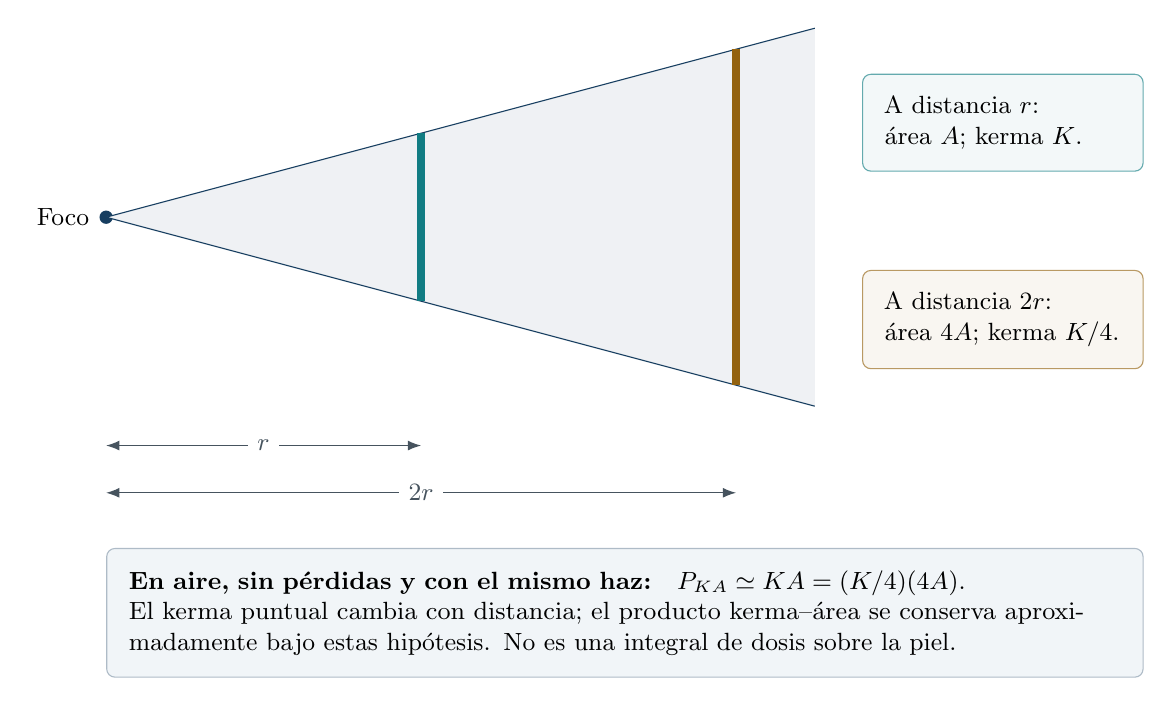
\begin{tikzpicture}[font=\small,x=1cm,y=1cm]
\node[punto,label=left:{Foco}]at(0,1){};
\fill[azul!7](0,1)--(9,3.4)--(9,-1.4)--cycle;
\draw[azul](0,1)--(9,3.4)(0,1)--(9,-1.4);
\draw[turquesa,line width=3pt](4,-.067)--(4,2.067);
\draw[ocre,line width=3pt](8,-1.133)--(8,3.133);
\draw[cota](0,-1.9)--(4,-1.9)node[midway,fill=white]{$r$};
\draw[cota](0,-2.5)--(8,-2.5)node[midway,fill=white]{$2r$};
\node[proceso,text width=3cm,anchor=west]at(9.6,2.2){A distancia $r$:\\área $A$; kerma $K$.};
\node[aviso,text width=3cm,anchor=west]at(9.6,-.3){A distancia $2r$:\\área $4A$; kerma $K/4$.};
\node[panel,text width=12.6cm,anchor=north west]at(0,-3.2){\textbf{En aire, sin pérdidas y con el mismo haz:}\quad $P_{KA}\simeq K A=(K/4)(4A)$.\\El kerma puntual cambia con distancia; el producto kerma--área se conserva aproximadamente bajo estas hipótesis. No es una integral de dosis sobre la piel.};
\end{tikzpicture}

\caption{Divergencia e inverso del cuadrado para un campo uniforme ideal. El esquema explica la diferencia entre kerma puntual y producto kerma--área; no incluye atenuación ni dispersión.}\label{fig:distancia_pka}\end{figure}

\section{Ecuación operativa por evento}
La expresión aplicada por el motor puede escribirse como
\begin{equation}\label{eq:dose}
D_e(\vect p)=M_e(\vect p)\,K_{\mathrm{a},r,e}
\left[\frac{d_{r,e}}{r_e(\vect p)}\right]^2
CF_e\,P_e(\vect p)\,T_e(\vect p)\,C_e(\vect p).
\end{equation}
La máscara $M_e$ selecciona primera entrada; $CF_e$ corrige el indicador; $P_e$ representa un perfil relativo; $T_e$ es transmisión de mesa y $C_e=B_e f_e$ representa la conversión dosimétrica superficial. En la tabla derivada, $C_e=B_e f_{\mathrm{eff},e}$, con una definición explícita de $f_{\mathrm{eff}}$.

Todos los términos salvo $\Ka$ son adimensionales. Sus factores requieren compatibilidad de normalización, plano de referencia y calidad del haz. 

\begin{table}[htbp]\centering\small
\caption{Etapas de cálculo y significado de su salida.}
\begin{tabularx}{\textwidth}{p{32mm}YY}\toprule
Etapa & Términos añadidos & Interpretación\\\midrule
\codigo{free_air} & $M_e$ y distancia. & Traslado geométrico del indicador de kerma, sin correcciones de equipo ni superficie.\\
\codigo{calibrated_air} & $CF$, perfil y mesa. & Estimación de kerma incidente corregido bajo la definición de esos factores.\\
\codigo{skin_dose} & $Bf$ o $C$. & Estimación superficial en el medio declarado, agua en el proveedor estudiado.\\\bottomrule
\end{tabularx}
\end{table}

\subsection{Identificación inequívoca de las salidas}
La magnitud se nombra según la etapa y el medio, no únicamente por su unidad. En esta memoria se utiliza \emph{máximo de kerma en aire trasladado} para \codigo{free_air}, \emph{máximo de kerma incidente corregido} para \codigo{calibrated_air} y \emph{máximo de dosis superficial modelada en agua} para \codigo{skin_dose} con el proveedor de agua. Ninguno de los dos primeros se denomina PSD en tejido.

La interfaz existente conserva el campo heredado \codigo{psd_point_gy}; esta edición documental no modifica el programa ni sus archivos de resultados. Al utilizar ese campo se deben comprobar conjuntamente \codigo{stage}, \codigo{quantity}, el medio declarado y el proveedor. No se presupone que el nombre heredado sea una definición física. La nomenclatura explícita recomendada para una futura actualización de la interfaz es:
\begin{itemize}[leftmargin=*]
\item \codigo{max_air_kerma_gy}: máximo de kerma en aire de la etapa indicada; distinguir traslado y corrección mediante \codigo{stage}.
\item \codigo{max_modeled_surface_dose_gy}: máximo superficial modelado, acompañado del medio y de las aproximaciones del proveedor.
\end{itemize}
Estos nombres son una propuesta de contrato de salida, no claves nuevas ya implementadas. Los informes y tablas de esta memoria emplean las denominaciones físicas anteriores; una salida en agua no se presenta como dosis absorbida en tejido a una profundidad clínica concreta sin justificación adicional.



\begin{figure}[htbp]\centering% Lectura término a término: magnitud inicial, correcciones y acumulación.
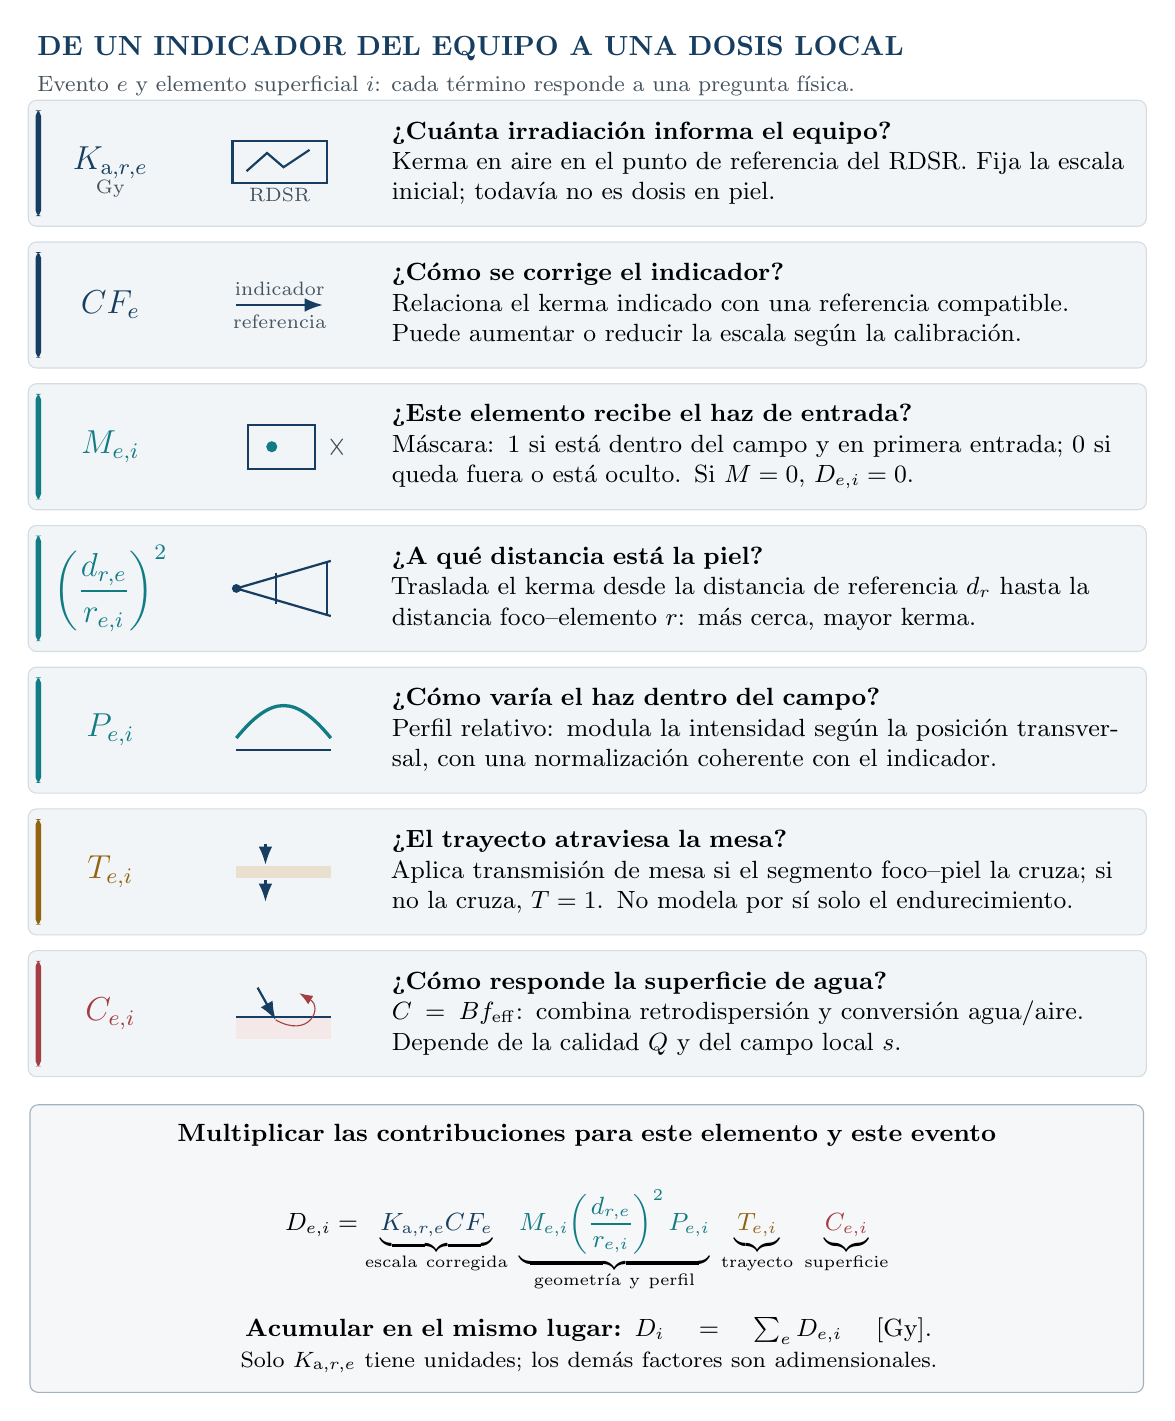
\begin{tikzpicture}[font=\small,
 card/.style={rounded corners=3pt,draw=azul!18,fill=gris,minimum width=14.2cm,minimum height=16mm},
 desc/.style={anchor=west,text width=9.3cm,align=left,font=\small},
 ico/.style={line width=.8pt,azul},
 lab/.style={font=\scriptsize,text=gristexto}]
\node[anchor=west,font=\bfseries\color{azul}] at (0,1.450) {DE UN INDICADOR DEL EQUIPO A UNA DOSIS LOCAL};
\node[anchor=west,font=\footnotesize,text=gristexto] at (0,0.980) {Evento $e$ y elemento superficial $i$: cada término responde a una pregunta física.};
% Filas independientes: símbolos, pictograma y función física.
\foreach \y/\col in {0/azul,-1.8/azul,-3.6/turquesa,-5.4/turquesa,-7.2/turquesa,-9/ocre,-10.8/rojo}{
 \node[card,anchor=west] at (0,\y) {};
 \fill[\col,rounded corners=2pt] (.10,\y-.67) rectangle (.17,\y+.67);
}
\node[text=azul,font=\large] at (1.05,0.000) {$K_{\mathrm a,r,e}$};
\node[lab] at (1.05,-0.320) {Gy};
\node[desc] at (4.5,0.000) {\textbf{¿Cuánta irradiación informa el equipo?}\\Kerma en aire en el punto de referencia del RDSR. Fija la escala inicial; todavía no es dosis en piel.};
\node[text=azul,font=\large] at (1.05,-1.800) {$CF_e$};
\node[desc] at (4.5,-1.800) {\textbf{¿Cómo se corrige el indicador?}\\Relaciona el kerma indicado con una referencia compatible. Puede aumentar o reducir la escala según la calibración.};
\node[text=turquesa,font=\large] at (1.05,-3.600) {$M_{e,i}$};
\node[desc] at (4.5,-3.600) {\textbf{¿Este elemento recibe el haz de entrada?}\\Máscara: $1$ si está dentro del campo y en primera entrada; $0$ si queda fuera o está oculto. Si $M=0$, $D_{e,i}=0$.};
\node[text=turquesa,font=\large] at (1.05,-5.400) {$\left(\dfrac{d_{r,e}}{r_{e,i}}\right)^2$};
\node[desc] at (4.5,-5.400) {\textbf{¿A qué distancia está la piel?}\\Traslada el kerma desde la distancia de referencia $d_r$ hasta la distancia foco--elemento $r$: más cerca, mayor kerma.};
\node[text=turquesa,font=\large] at (1.05,-7.200) {$P_{e,i}$};
\node[desc] at (4.5,-7.200) {\textbf{¿Cómo varía el haz dentro del campo?}\\Perfil relativo: modula la intensidad según la posición transversal, con una normalización coherente con el indicador.};
\node[text=ocre,font=\large] at (1.05,-9.000) {$T_{e,i}$};
\node[desc] at (4.5,-9.000) {\textbf{¿El trayecto atraviesa la mesa?}\\Aplica transmisión de mesa si el segmento foco--piel la cruza; si no la cruza, $T=1$. No modela por sí solo el endurecimiento.};
\node[text=rojo,font=\large] at (1.05,-10.800) {$C_{e,i}$};
\node[desc] at (4.5,-10.800) {\textbf{¿Cómo responde la superficie de agua?}\\$C=Bf_{\mathrm{eff}}$: combina retrodispersión y conversión agua/aire. Depende de la calidad $Q$ y del campo local $s$.};
% Miniaturas didácticas: no son resultados de transporte.
\draw[ico] (2.6,-0.250) rectangle (3.8,0.280);
\draw[ico] (2.78,-0.100)--(3.04,0.130)--(3.25,-0.050)--(3.58,0.170);
\node[lab] at (3.2,-0.400) {RDSR};
\draw[ico,-{Latex}] (2.65,-1.800)--(3.75,-1.800);
\node[lab,above] at (3.2,-1.800) {indicador};
\node[lab,below] at (3.2,-1.800) {referencia};
\draw[ico] (2.8,-3.880)--(2.8,-3.320)--(3.65,-3.320)--(3.65,-3.880)--cycle;
\fill[turquesa] (3.1,-3.600) circle (2pt);
\draw[gristexto] (3.85,-3.500)--(4,-3.700) (3.85,-3.700)--(4,-3.500);
\fill[azul] (2.65,-5.400) circle (1.6pt);
\draw[ico] (2.65,-5.400)--(3.85,-5.050) (2.65,-5.400)--(3.85,-5.750);
\draw[ico] (3.15,-5.600)--(3.15,-5.200) (3.8,-5.750)--(3.8,-5.050);
\draw[ico] (2.65,-7.450)--(3.85,-7.450);
\draw[turquesa,line width=1.2pt] (2.65,-7.300)..controls (3.1,-6.750) and (3.4,-6.750)..(3.85,-7.300);
\fill[ocre!20] (2.65,-9.080) rectangle (3.85,-8.920);
\draw[ico,-{Latex}] (3.02,-8.650)--(3.02,-8.910);
\draw[ico,-{Latex}] (3.02,-9.100)--(3.02,-9.380);
\draw[ico] (2.65,-10.850)--(3.85,-10.850);
\fill[rojo!12] (2.65,-10.850) rectangle (3.85,-11.120);
\draw[ico,-{Latex}] (2.92,-10.470)--(3.15,-10.880);
\draw[rojo,-{Latex}] (3.15,-10.880)..controls (3.58,-11.120) and (3.75,-10.720)..(3.45,-10.540);
% Synthèse: produit local puis somme des événements.
\node[draw=azul!40,fill=azul!4,rounded corners=3pt,text width=13.65cm,align=center,inner sep=7pt,anchor=north] at (7.1,-11.950) {
\textbf{Multiplicar las contribuciones para este elemento y este evento}\\[-1mm]
\[D_{e,i}=\underbrace{\color{azul}K_{\mathrm a,r,e}CF_e}_{\text{escala corregida}}\;
\underbrace{\color{turquesa}M_{e,i}\!\left(\frac{d_{r,e}}{r_{e,i}}\right)^2P_{e,i}}_{\text{geometría y perfil}}\;
\underbrace{\color{ocre}T_{e,i}}_{\text{trayecto}}\;
\underbrace{\color{rojo}C_{e,i}}_{\text{superficie}}\]
\textbf{Acumular en el mismo lugar:} $D_i=\sum_e D_{e,i}$ \quad [Gy].\\
\footnotesize Solo $K_{\mathrm a,r,e}$ tiene unidades; los demás factores son adimensionales.};
\end{tikzpicture}

\caption{Contribución física de los siete términos de la ecuación operativa. El producto determina la dosis de un evento en un elemento; la suma acumula eventos en ese mismo lugar. Los pictogramas son esquemas didácticos, no simulaciones de transporte.}\label{fig:ecuacion}\end{figure}

\FloatBarrier
\subsection{Interpretación dosimétrica formal de los factores}
\label{sec:factores-formal}
La Figura~\ref{fig:ecuacion} proporciona una lectura cualitativa. Formalmente, la Ecuación~\eqref{eq:dose} aproxima la dosis superficial mediante una factorización del kerma incidente y de la respuesta del medio. Para un elemento $i$, situado en $\vect p_i$, conviene distinguir
\begin{align}
K^{\mathrm{inc}}_{a,e,i}&=K_{\mathrm a,r,e}\,CF_e
\left(\frac{d_{r,e}}{r_{e,i}}\right)^2P_{e,i}T_{e,i},\label{eq:kerma-local-formal}\\
D_{w,e,i}&\simeq M_{e,i}\,K^{\mathrm{inc}}_{a,e,i}\,C_{e,i}.
\label{eq:dosis-local-formal}
\end{align}
Aquí $K^{\mathrm{inc}}_a$ designa el kerma en aire del haz incidente en la localización superficial, excluyendo la retrodispersión del paciente; $D_w$ designa la magnitud superficial referida al agua bajo las condiciones del proveedor. Esta separación es conceptual: no implica que el programa resuelva el espectro incidente ni el transporte secundario para cada cara. La factorización requiere definiciones compatibles de referencia, campo, calidad y medio~\citep{aapm2021,benreport}.

\paragraph{Indicador y calibración: $K_{\mathrm a,r,e}$ y $CF_e$.}
El indicador del evento establece la normalización absoluta en Gy en un punto de referencia del sistema, no en la piel. Una definición operativa de la corrección de calibración es
\begin{equation}
CF_e=\frac{K^{\mathrm{ref}}_{a,r,e}}{K^{\mathrm{ind}}_{a,r,e}},
\qquad K^{\mathrm{ind}}_{a,r,e}=K_{\mathrm a,r,e}.
\end{equation}
Numerador y denominador deben corresponder a la misma irradiación y a una referencia compatible. La corrección puede depender de calidad del haz y modo de adquisición. Por ello, $CF=1$ puede ser una hipótesis de demostración y no evidencia de calibración exacta.

\paragraph{Selección espacial: $M_{e,i}$.}
La máscara binaria representa la pertenencia del elemento al campo primario y su condición de primera intersección del rayo con la superficie. En el modelo idealizado,
\begin{equation}
M_{e,i}=\mathbf 1_{\{\text{dentro del campo}\}}(i)\,
\mathbf 1_{\{\text{primera entrada}\}}(i).
\end{equation}
No es una probabilidad de interacción. Su valor nulo excluye la contribución de ese evento en la formulación implementada. Con una muestra en el centroide, una cara parcialmente incluida se clasifica mediante ese punto, lo que introduce dependencia de la discretización.

\paragraph{Divergencia geométrica: $(d_{r,e}/r_{e,i})^2$.}
La ley del inverso del cuadrado procede de la dilución de fluencia en propagación desde una fuente puntual, manteniendo el ángulo sólido y la calidad del haz. El cociente compara la distancia fuente--referencia con la distancia euclídea fuente--elemento. No debe sustituirse esta última por la profundidad axial o por la distancia fuente--isocentro. La ley utilizada no incluye atenuación en aire, tamaño focal finito ni dispersión. Tampoco se añade un coseno de incidencia al kerma puntual: la oblicuidad modifica la huella y las áreas geométricas, y una dependencia dosimétrica angular adicional requiere un modelo específico.

\paragraph{No uniformidad transversal: $P_{e,i}$.}
El perfil expresa una relación de kerma respecto a una posición de normalización. Puede definirse, a una distancia de caracterización común $d_0$, como
\begin{equation}
P_e(u,v)=\frac{K^{\mathrm{libre}}_{a,e}(u,v;d_0)}
{K^{\mathrm{libre}}_{a,e}(0,0;d_0)},
\qquad P_e(0,0)=1,
\end{equation}
cuando el eje central sea la referencia adoptada. La asignación al elemento se realiza mediante sus coordenadas transversales proyectadas. Esta definición separa perfil y distancia para evitar aplicar dos veces la divergencia. Un perfil escalar de amplitud no describe por sí solo la variación espacial del espectro, aunque reproduzca parte de la no uniformidad de kerma.

\paragraph{Transmisión del soporte: $T_{e,i}$.}
La transmisión relevante para esta factorización es una razón de kerma incidente, con y sin el conjunto mesa/colchón caracterizado, en condiciones geométricas compatibles:
\begin{equation}
T_{e,i}=\frac{K^{\mathrm{con\ soporte}}_{a,e,i}}
{K^{\mathrm{sin\ soporte}}_{a,e,i}}.
\end{equation}
Se aplica solo cuando el soporte intersecta el trayecto anterior a la entrada. Para un modelo puramente atenuador se espera $0<T\leq1$; si no hay cruce, $T=1$. La transmisión efectiva depende de calidad y ángulo, y su definición experimental debe especificar la contribución dispersa aceptada. La aproximación escalar del motor reduce amplitud sin actualizar la calidad usada en el factor superficial: ese acoplamiento espectral permanece fuera de esta operación.

\paragraph{Respuesta superficial del agua: $C_{e,i}$.}
En la ecuación 13 de la fuente, el factor combinado convierte kerma en aire libre en kerma en agua en la superficie del fantoma. Interpretarlo como dosis absorbida requiere las aproximaciones de equilibrio electrónico y pérdidas radiativas despreciables del formalismo. No define una profundidad cutánea clínica ni resuelve el desequilibrio en una interfaz arbitraria. En la construcción espectral del proyecto se conserva el formalismo de Benmakhlouf~\citep{benreport}:
\begin{equation}
C(Q,s)=\frac{\int k_a(E;Q)\,B(E,s)f(E,s)\,\mathrm dE}
{\int k_a(E;Q)\,\mathrm dE},
\qquad k_a(E;Q)\propto E\Phi(E;Q)\muen{a}(E).
\end{equation}
$k_a$ es la densidad espectral de kerma empleada con la convención del informe; $B$ y $f$ mantienen sus definiciones monoenergéticas de la fuente. El factor usado es adimensional y depende tanto del espectro como del tamaño de campo. Se define $f_{\mathrm{eff}}(Q,s)=C(Q,s)/B(Q,s)$ para conservar la interfaz multiplicativa; no es, en general, el promedio independiente de $f(E,s)$ ni un cociente evaluado a una energía media. La aplicación local de factores centrales de un fantoma de agua a una anatomía curva es una aproximación del modelo, no una simulación de retrodispersión anatómica.

\paragraph{Acumulación y alcance de la respuesta.}
La dosis acumulada se obtiene por superposición de contribuciones sobre el mismo elemento material representado: $D_{w,i}=\sum_eD_{w,e,i}$. La suma presupone una correspondencia anatómica válida entre eventos. Traslaciones de mesa conocidas no describen por sí solas movimientos o deformaciones del paciente respecto a ella. La magnitud resultante sigue siendo una estimación superficial en el medio declarado, sin una profundidad cutánea asignada ni una distribución de dosis de salida. Las contribuciones multiplicativas no son incertidumbres independientes: una misma calidad del haz puede afectar simultáneamente a $CF$, $P$, $T$ y $C$.

\section{Calibración, perfil y mesa}
El factor $CF$ debe relacionar el indicador con una referencia de kerma en la misma geometría y sin incorporar correcciones que el motor aplicará después. Puede depender de modo y calidad. Los valores $CF=1$ de demostración no evidencian calibración perfecta: expresan ausencia de una corrección medida.

El perfil $P$ permite modificar la distribución transversal. Su normalización debe ser consistente con el punto donde se define $\Ka$. Una función relativa cuyo valor central no corresponde a esa normalización puede cambiar toda la escala de dosis. El efecto talón no aparece automáticamente por usar un ánodo de tungsteno en los factores centrales; requiere una representación espacial o espectral fuera del eje.

La transmisión se aplica únicamente si el segmento foco--superficie cruza la mesa antes del punto de entrada. El código admite una transmisión total o el producto de una parte normal y otra angular, evitando la coexistencia de ambas parametrizaciones. La configuración de investigación emplea $T=\num{0.8}$ para los rayos que cruzan la mesa y corrección angular unidad. Son valores sintéticos.

Aplicar una transmisión escalar reduce amplitud, pero no endurece el espectro usado para $C$. En el equipo real la mesa puede cambiar ambas cosas. Una futura implementación coherente debería usar el espectro transmitido para los factores correspondientes o un factor efectivo medido con la misma definición, sin duplicar la atenuación.



\begin{figure}[htbp]\centering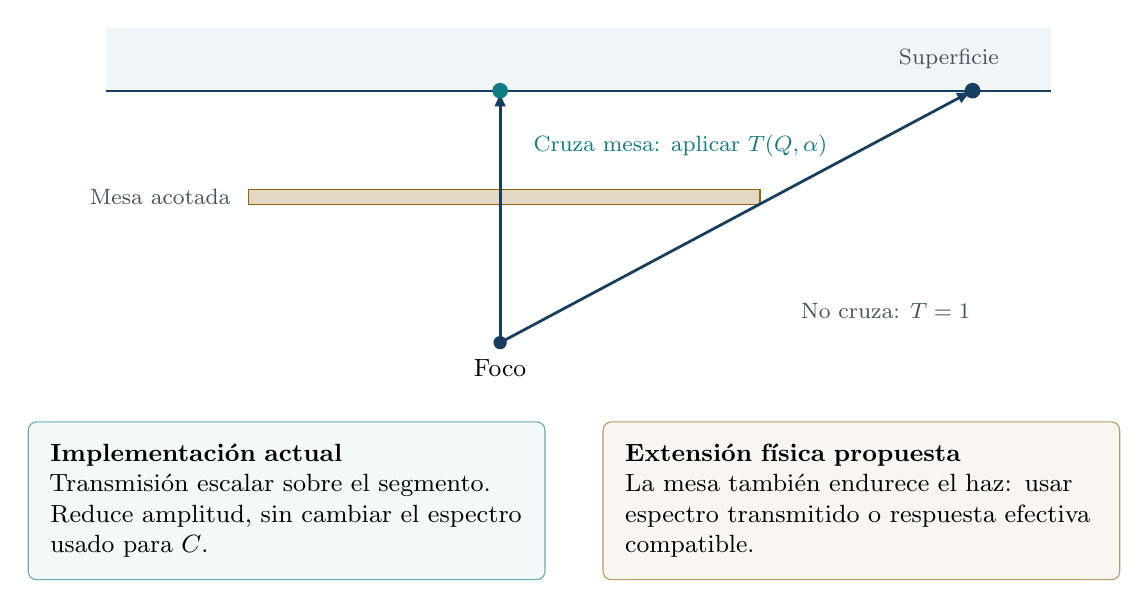
\begin{tikzpicture}[font=\small,x=1cm,y=1cm]
\fill[gris](1,2.2)rectangle(13,3);\draw[azul,thick](1,2.2)--(13,2.2);
\node[nota]at(11.7,2.6){Superficie};
\fill[ocre!25](2.8,.75)rectangle(9.3,.95);\draw[ocre](2.8,.75)rectangle(9.3,.95);
\node[nota,anchor=east]at(2.7,.85){Mesa acotada};
\node[punto,label=below:{Foco}]at(6,-1){};
\draw[rayo](6,-1)--(6,2.2);\node[circle,fill=turquesa,inner sep=2pt]at(6,2.2){};
\draw[rayo](6,-1)--(12,2.2);\node[circle,fill=azul,inner sep=2pt]at(12,2.2){};
\node[nota,text=turquesa,anchor=west]at(6.3,1.5){Cruza mesa: aplicar $T(Q,\alpha)$};
\node[nota,anchor=west]at(9.7,-.6){No cruza: $T=1$};
\node[proceso,text width=6cm,anchor=north west]at(0,-2){\textbf{Implementación actual}\\Transmisión escalar sobre el segmento. Reduce amplitud, sin cambiar el espectro usado para $C$.};
\node[aviso,text width=6cm,anchor=north west]at(7.3,-2){\textbf{Extensión física propuesta}\\La mesa también endurece el haz: usar espectro transmitido o respuesta efectiva compatible.};
\end{tikzpicture}

\caption{La transmisión depende del trayecto antes de la primera entrada. Se distingue el factor escalar implementado de una futura respuesta que incluya endurecimiento; sin espesores ni transmisión medidos en el dibujo.}\label{fig:mesa}\end{figure}

\section{Retrodispersión y lo que queda fuera del campo}
La retrodispersión eleva la respuesta superficial respecto al haz incidente en las condiciones del fantoma. El factor tabulado representa una respuesta central para una geometría concreta, no un campo disperso resuelto espacialmente. El motor conserva exactamente cero fuera de la máscara primaria para cada evento.

Por ello, un mapa con borde neto no demuestra que la dispersión física sea nula fuera del campo. Tampoco incluye dosis de salida ni contribuciones de órganos internos. Estas exclusiones son propiedades de la formulación actual, no defectos gráficos que se resuelvan suavizando colores o aumentando triángulos.

\Needspace{12cm}
\section{Acumulación y máximo}
Las contribuciones se suman sobre elementos homólogos de la misma superficie:
\begin{equation}
D(\vect p_i)=\sum_e D_e(\vect p_i),\qquad
\mathrm{PSD}_{\mathrm{puntual}}=\max_i D(\vect p_i).
\end{equation}
En general, $\max_i\sum_eD_e(\vect p_i)\neq\sum_e\max_iD_e(\vect p_i)$. La segunda expresión puede sobreestimar el máximo acumulado cuando los campos se sitúan en regiones diferentes.
\begin{figure}[H]\centering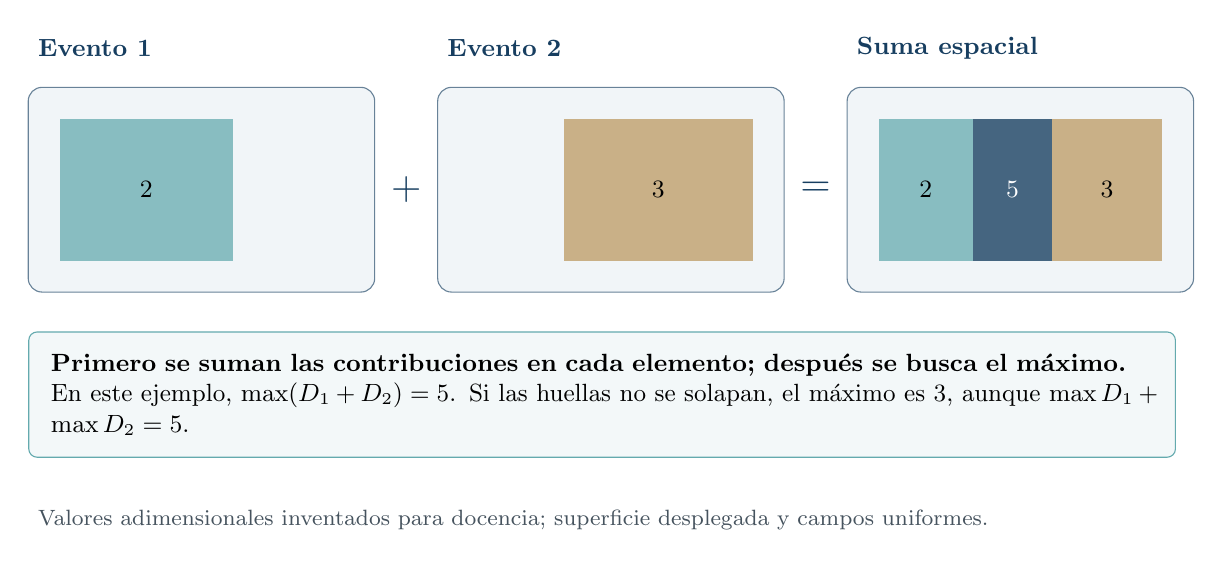
\begin{tikzpicture}[x=1cm,y=1cm,font=\small]
\foreach \x/\titre in {0/{Evento 1},5.2/{Evento 2},10.4/{Suma espacial}}{
\node[rotulo,anchor=west]at(\x,3.1){\titre};
\draw[azul!65,rounded corners=5pt,fill=gris](\x,0)rectangle++(4.4,2.6);}
\fill[turquesa!50](.4,.4)rectangle(2.6,2.2);
\fill[ocre!50](6.8,.4)rectangle(9.2,2.2);
\fill[turquesa!50](10.8,.4)rectangle(13,2.2);
\fill[ocre!50](12,.4)rectangle(14.4,2.2);
\fill[azul!80](12,.4)rectangle(13,2.2);
\node at(1.5,1.3){$2$};\node at(8,1.3){$3$};
\node at(11.4,1.3){$2$};\node[text=white]at(12.5,1.3){$5$};\node at(13.7,1.3){$3$};
\node[font=\Large,text=azul]at(4.8,1.3){$+$};\node[font=\Large,text=azul]at(10,1.3){$=$};
\node[proceso,text width=14cm,anchor=north west]at(0,-.5){\textbf{Primero se suman las contribuciones en cada elemento; después se busca el máximo.}\\En este ejemplo, $\max(D_1+D_2)=5$. Si las huellas no se solapan, el máximo es $3$, aunque $\max D_1+\max D_2=5$.};
\node[nota,anchor=north west]at(0,-2.65){Valores adimensionales inventados para docencia; superficie desplegada y campos uniformes.};
\end{tikzpicture}

\caption{Acumulación espacial y superposición. Esquema TikZ, sin valores dosimétricos ni anatomía clínica.}\end{figure}
\FloatBarrier

\chapter{Geometría del haz y discretización superficial}
\section{Sistemas de referencia}
La reconstrucción utiliza marcos de equipo, mesa y superficie. El sistema interno de la superficie adopta $x$ hacia la izquierda del paciente, $y$ craneal y $z$ anterior. El archivo de malla puede utilizar otros ejes, por lo que la transformación de importación debe declararse. Un STL no contiene una convención anatómica ni unidades inequívocas.

La transformación puede expresarse como $\vect p_{\mathrm{int}}=R_{\mathrm{malla}}\vect p_{\mathrm{archivo}}+\vect o_{\mathrm{malla}}$, junto con el factor de escala de unidad cuando procede. La traslación relativa paciente--mesa se aplica de manera coherente con el desplazamiento del equipo. Los signos de las rotaciones y su orden deben pertenecer a un perfil identificado, no deducirse de la apariencia visual.

En el cálculo de malla, mantener la superficie en su marco y llevar el foco a ese marco evita reconstruir el índice de intersección para cada desplazamiento de mesa. La transformación cambia las coordenadas del problema, sin cambiar la intersección física que se desea resolver. Una caché solo puede reutilizar resultados si la geometría relevante coincide.



\begin{figure}[htbp]\centering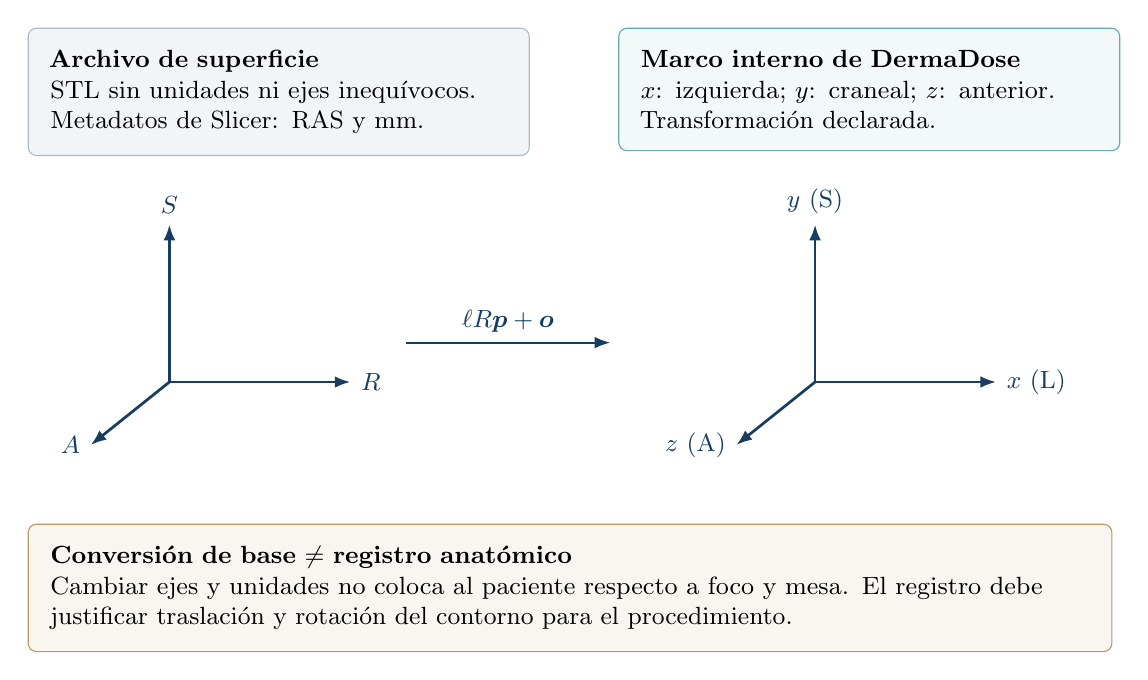
\begin{tikzpicture}[font=\small,x=1cm,y=1cm]
\node[panel,text width=5.8cm,anchor=north west]at(0,4.3){\textbf{Archivo de superficie}\\STL sin unidades ni ejes inequívocos. Metadatos de Slicer: RAS y mm.};
\node[proceso,text width=5.8cm,anchor=north west]at(7.5,4.3){\textbf{Marco interno de DermaDose}\\$x$: izquierda; $y$: craneal; $z$: anterior. Transformación declarada.};
\coordinate(O)at(1.8,-.2);\draw[rayo](O)--++(2.3,0)node[right]{$R$};\draw[rayo](O)--++(0,2)node[above]{$S$};\draw[rayo](O)--++(-1,-.8)node[left]{$A$};
\coordinate(I)at(10,-.2);\draw[rayo](I)--++(2.3,0)node[right]{$x$ (L)};\draw[rayo](I)--++(0,2)node[above]{$y$ (S)};\draw[rayo](I)--++(-1,-.8)node[left]{$z$ (A)};
\draw[flujo](4.8,.3)--(7.4,.3)node[midway,above]{$\ell R\vect p+\vect o$};
\node[aviso,text width=13.2cm,anchor=north west]at(0,-2){\textbf{Conversión de base $\neq$ registro anatómico}\\Cambiar ejes y unidades no coloca al paciente respecto a foco y mesa. El registro debe justificar traslación y rotación del contorno para el procedimiento.};
\end{tikzpicture}

\caption{Relación entre convenciones de coordenadas. Los triedros son simbólicos: la transformación cambia componentes y unidades; el registro establece la posición física. No se propone una matriz automática para cualquier STL.}\label{fig:coordenadas}\end{figure}

\section{Foco, eje y campo rectangular divergente}
Sea $\vect b_e$ el eje unitario, y $\vect u_e,\vect v_e$ sus direcciones transversales. Para $\vect\Delta=\vect p-\vect s_e$, la profundidad axial es $t_e=\vect\Delta\cdot\vect b_e$. Si las dimensiones $w_e,h_e$ se declaran a distancia $d_{f,e}$, las condiciones de campo son
\begin{equation}\label{eq:field}
0<t_e\leq\mathrm{SID}_e,\qquad
|\vect\Delta\cdot\vect u_e|\leq\frac{w_e t_e}{2d_{f,e}},\qquad
|\vect\Delta\cdot\vect v_e|\leq\frac{h_e t_e}{2d_{f,e}}.
\end{equation}
La configuración distingue referencia en detector o isocentro. La profundidad $t_e$ controla la apertura; la distancia euclídea $r_e$ controla el inverso del cuadrado. Son iguales solo sobre el eje.
\begin{figure}[htbp]\centering\resizebox{.96\textwidth}{!}{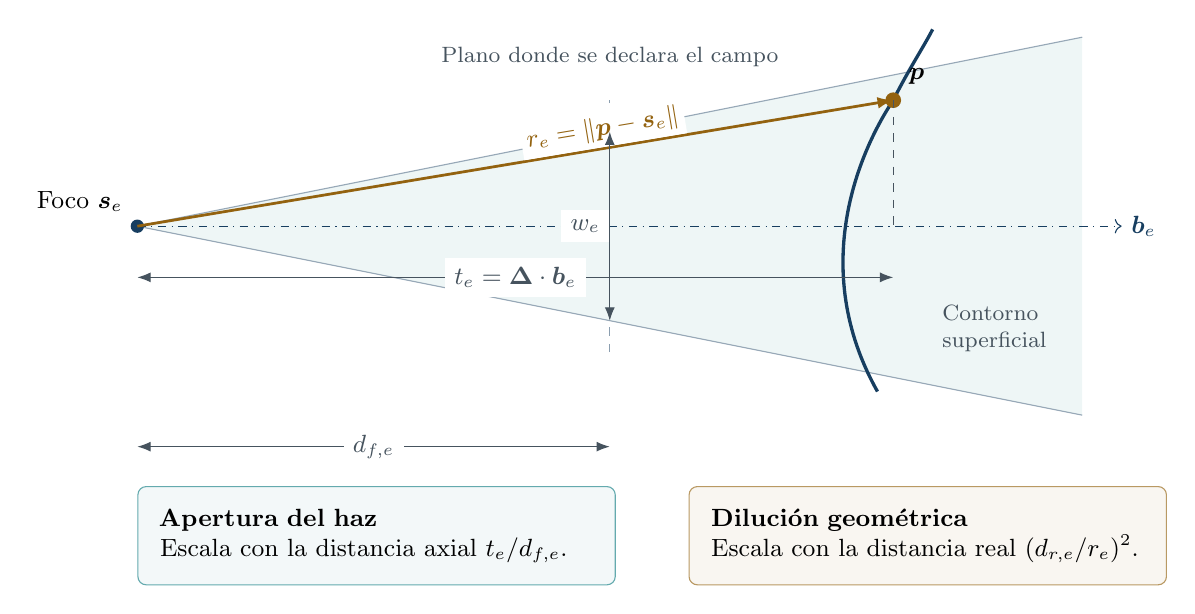
\begin{tikzpicture}[x=1cm,y=1cm,font=\small]
\fill[turquesa!7] (0,0)--(12,2.4)--(12,-2.4)--cycle;
\draw[azul!45] (0,0)--(12,2.4) (0,0)--(12,-2.4);
\draw[azul,dash dot,->] (0,0)--(12.5,0) node[right]{$\vect b_e$};
\draw[azul!50,dashed] (6,-1.6)--(6,1.6);
\draw[very thick,azul] (9.4,-2.1)..controls(8.5,-.5)and(9.2,1)..(9.6,1.6)..controls(9.8,2)and(10,2.3)..(10.1,2.5);
\coordinate(S)at(0,0);\coordinate(P)at(9.6,1.6);
\node[punto,label=above left:{Foco $\vect s_e$}]at(S){};
\draw[rayo,ocre] (S)--(P) node[pos=.62,above,sloped,fill=white,inner sep=2pt]{$r_e=\|\vect p-\vect s_e\|$};
\node[circle,fill=ocre,inner sep=2pt,label=above right:{$\vect p$}]at(P){};
\draw[dashed,gristexto](P)--(9.6,0);
\draw[cota](0,-.65)--(9.6,-.65) node[midway,fill=white]{$t_e=\vect\Delta\cdot\vect b_e$};
\draw[cota](0,-2.8)--(6,-2.8) node[midway,fill=white]{$d_{f,e}$};
\draw[cota](6,-1.2)--(6,1.2) node[midway,left,fill=white]{$w_e$};
\node[nota,anchor=south]at(6,1.9){Plano donde se declara el campo};
\node[nota,anchor=west]at(10.1,-1.3){Contorno\\superficial};
\node[proceso,text width=5.5cm,anchor=north west]at(0,-3.3){\textbf{Apertura del haz}\\Escala con la distancia axial $t_e/d_{f,e}$.};
\node[aviso,text width=5.5cm,anchor=north west]at(7,-3.3){\textbf{Dilución geométrica}\\Escala con la distancia real $(d_{r,e}/r_e)^2$.};
\end{tikzpicture}
}
\caption{Distancias axial y euclídea en un haz divergente. El contorno es esquemático y no representa el registro XCAT de trabajo.}\end{figure}

La sección normal al haz a esa profundidad es
\begin{equation}
A_{\perp,e}(\vect p)=\frac{w_e h_e}{100}\left(\frac{t_e}{d_{f,e}}\right)^2\quad[\mathrm{cm^2}],
\end{equation}
con dimensiones originales en mm. Esta área se usa como argumento de los factores. No es el área de la huella sobre una piel inclinada, ni la suma de áreas de triángulos irradiados.



\begin{figure}[htbp]\centering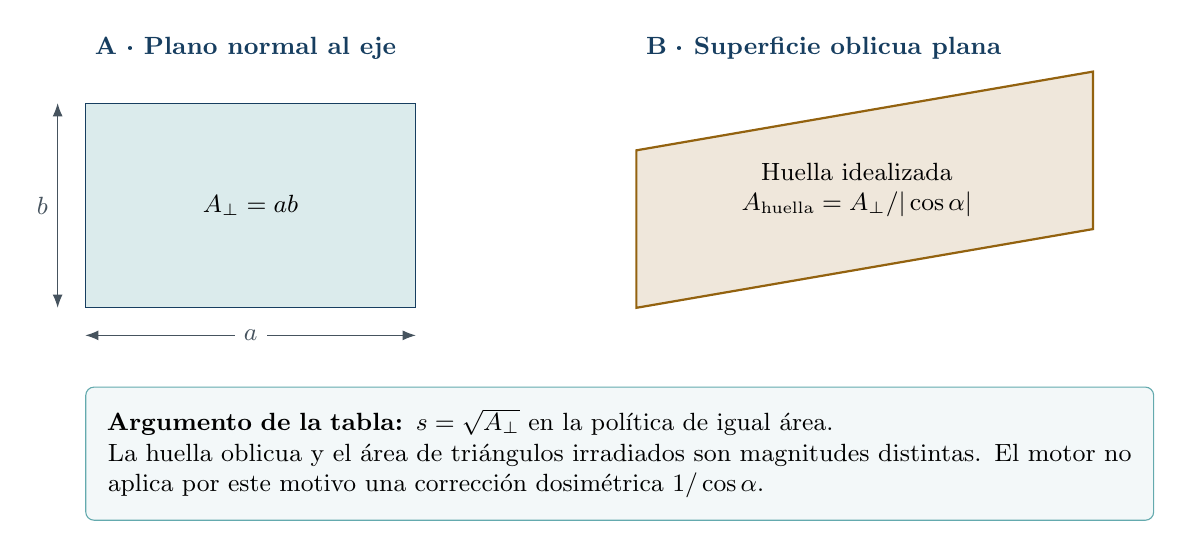
\begin{tikzpicture}[font=\small,x=1cm,y=1cm]
\node[rotulo,anchor=west]at(0,3.3){A · Plano normal al eje};
\draw[azul,fill=turquesa!15](0,0)rectangle(4.2,2.6);
\draw[cota](0,-.35)--(4.2,-.35)node[midway,fill=white]{$a$};
\draw[cota](-.35,0)--(-.35,2.6)node[midway,left]{$b$};
\node at(2.1,1.3){$A_\perp=ab$};
\node[rotulo,anchor=west]at(7,3.3){B · Superficie oblicua plana};
\fill[ocre!15](7,0)--(12.8,1)--(12.8,3)--(7,2)--cycle;
\draw[ocre,thick](7,0)--(12.8,1)--(12.8,3)--(7,2)--cycle;
\node[align=center]at(9.8,1.5){Huella idealizada\\$A_{\rm huella}=A_\perp/|\cos\alpha|$};
\node[proceso,text width=13cm,anchor=north west]at(0,-1){\textbf{Argumento de la tabla:} $s=\sqrt{A_\perp}$ en la política de igual área.\\La huella oblicua y el área de triángulos irradiados son magnitudes distintas. El motor no aplica por este motivo una corrección dosimétrica $1/\cos\alpha$.};
\end{tikzpicture}

\caption{Tres áreas con funciones distintas. La relación de proyección de la huella supone un haz localmente paralelo y un plano; no se extrapola directamente a una superficie curva o a un haz de divergencia finita.}\label{fig:areas_campo}\end{figure}

\section{Orientación y primera intersección}
Una normal dirigida al foco es una condición necesaria de entrada, pero no suficiente. Un brazo puede ocultar parte del tronco y una concavidad puede contener caras orientadas al foco que no reciben el haz primario directamente. La máscara combina preselección por campo y orientación con la primera intersección positiva del rayo.

El trazado utiliza Trimesh y un índice R-tree sobre la geometría. Es un algoritmo geométrico en CPU, sin transporte fotónico ni electrónica secundaria. La selección de primera entrada excluye las superficies de salida y las caras ocultas. Las tolerancias cerca de vértices y aristas merecen ensayos propios, porque una decisión de intersección degenerada puede cambiar la máscara.

Las normales también proporcionan el ángulo de incidencia. No se multiplica automáticamente la dosis por un coseno. El cambio de orientación altera la región interceptada y el área geométrica; una corrección angular dosimétrica debe estar sustentada por medidas o por un cálculo compatible. En el proveedor de agua estudiado, la transferencia local de datos de incidencia normal sigue siendo una aproximación.



\begin{figure}[htbp]\centering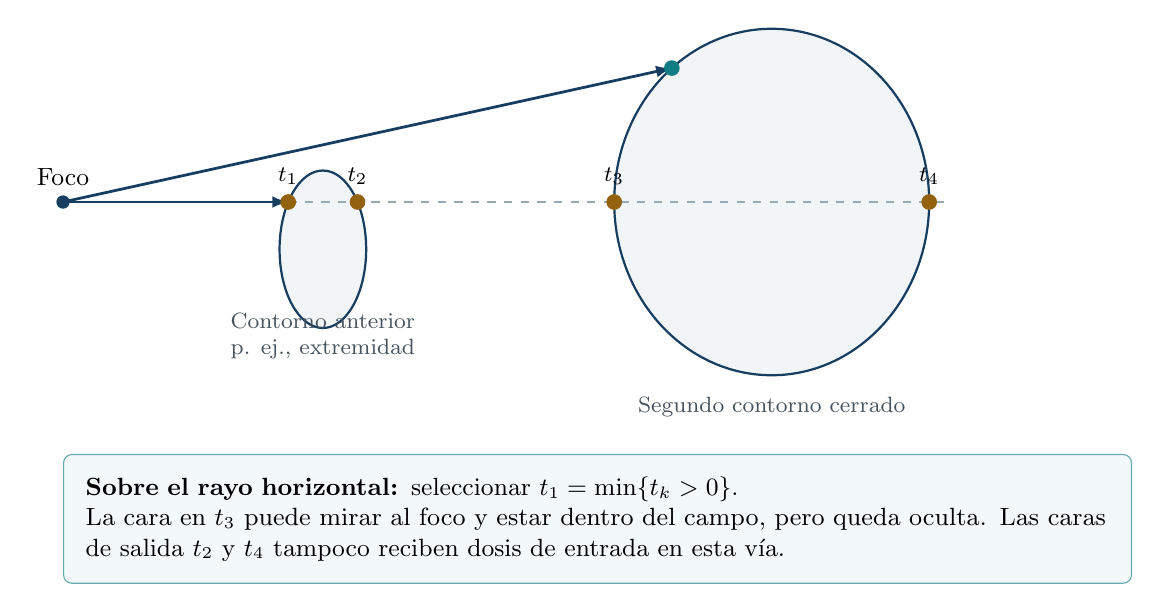
\begin{tikzpicture}[font=\small,x=1cm,y=1cm]
\fill[gris](3.3,-.6)ellipse(.55 and 1);\draw[azul,thick](3.3,-.6)ellipse(.55 and 1);
\fill[gris](9,0)ellipse(2 and 2.2);\draw[azul,thick](9,0)ellipse(2 and 2.2);
\node[punto,label=above:{Foco}]at(0,0){};
\draw[rayo](0,0)--(2.86,0);\draw[azul!45,dashed](2.86,0)--(11.2,0);
\foreach \x/\n in {2.86/1,3.74/2,7/3,11/4}{\node[circle,fill=ocre,inner sep=2pt]at(\x,0){};\node[font=\footnotesize,above]at(\x,.1){$t_\n$};}
\draw[rayo](0,0)--(7.7316,1.701);
\node[circle,fill=turquesa,inner sep=2pt]at(7.7316,1.701){};
\node[nota,align=center]at(3.3,-1.7){Contorno anterior\\p. ej., extremidad};
\node[nota]at(9,-2.6){Segundo contorno cerrado};
\node[proceso,text width=13cm,anchor=north west]at(0,-3.2){\textbf{Sobre el rayo horizontal:} seleccionar $t_1=\min\{t_k>0\}$.\\La cara en $t_3$ puede mirar al foco y estar dentro del campo, pero queda oculta. Las caras de salida $t_2$ y $t_4$ tampoco reciben dosis de entrada en esta vía.};
\end{tikzpicture}

\caption{Primera intersección positiva en un corte esquemático. Una normal orientada al foco no basta para excluir oclusión. No se simula transmisión a través de la primera región corporal.}\label{fig:primera_entrada}\end{figure}

\section{Malla de cálculo y punto representativo}
Cada cara triangular dispone de centroide, normal y área. La dosis evaluada en el centroide se considera representativa de toda la cara. La regla es simple y permite sumar áreas, pero introduce error en bordes abruptos de campo o de mesa: un triángulo parcialmente cubierto puede contarse completamente dentro o fuera.

La calidad de muestreo depende del tamaño local, forma y distribución de caras. Dos mallas de \num{150000} triángulos pueden tener distinta resolución en la región irradiada. Por ello, el número de triángulos es un presupuesto de cálculo y no una especificación de exactitud. Conviene acompañarlo de distribución de aristas, áreas, calidad de forma y prueba de convergencia.

El parámetro \codigo{mesh_max_edge_mm} subdivide caras largas y mantiene el poliedro de origen. No recupera una curvatura que el STL no representaba. El parámetro general \codigo{resolution_mm} no subdivide por sí solo una malla importada. La distinción evita interpretar una configuración nominal de 5 mm como garantía sobre todos sus elementos.



\begin{figure}[htbp]\centering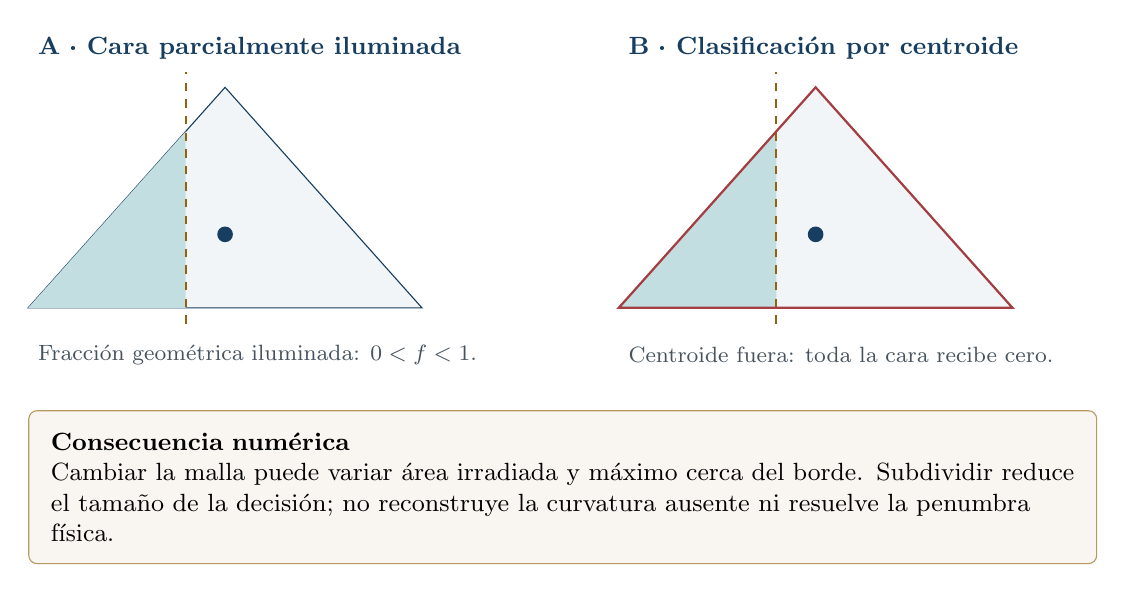
\begin{tikzpicture}[font=\small,x=1cm,y=1cm]
\foreach \x/\titre in {0/{A · Cara parcialmente iluminada},7.5/{B · Clasificación por centroide}}{
\node[rotulo,anchor=west]at(\x,3.3){\titre};
\draw[azul,fill=gris](\x,0)--++(5,0)--++(-2.5,2.8)--cycle;
\fill[turquesa!25](\x,0)--++(2,0)--++(0,2.24)--cycle;
\draw[ocre,dashed,thick](\x+2,-.2)--(\x+2,3);
\node[circle,fill=azul,inner sep=2pt]at(\x+2.5,.933){};}
\draw[rojo,thick](7.5,0)--(12.5,0)--(10,2.8)--cycle;
\node[nota,anchor=west]at(0,-.6){Fracción geométrica iluminada: $0<f<1$.};
\node[nota,anchor=west]at(7.5,-.6){Centroide fuera: toda la cara recibe cero.};
\node[aviso,text width=13cm,anchor=north west]at(0,-1.3){\textbf{Consecuencia numérica}\\Cambiar la malla puede variar área irradiada y máximo cerca del borde. Subdividir reduce el tamaño de la decisión; no reconstruye la curvatura ausente ni resuelve la penumbra física.};
\end{tikzpicture}

\caption{Ejemplo de muestreo binario en una cara cruzada por el campo. La zona turquesa muestra la porción geométrica iluminada; el punto azul representa el centroide. No se calcula intersección parcial de área en la regla descrita.}\label{fig:centroides}\end{figure}

\section{Subdivisión frente a simplificación}
La subdivisión aumenta el muestreo conservando cada plano triangular. La simplificación elimina caras y puede modificar la forma. Ambas operaciones requieren evaluaciones diferentes. Para la primera interesan estabilidad de PSD, áreas e integral; para la segunda deben añadirse distancias entre superficies, cambios de volumen y conservación de rasgos relevantes para sombras y distancias.

Una simplificación topológicamente válida puede desplazar el contorno. A la inversa, una malla visualmente parecida puede contener agujeros o caras invertidas que invalidan la primera entrada. Los controles de cierre y conectividad son necesarios, pero no demuestran fidelidad anatómica ni ausencia completa de autointersecciones.

\section{Mesa, movimiento y barridos}
La mesa se representa mediante un plano rectangular acotado. El cruce se evalúa en el segmento foco--punto y se verifica que ocurra antes de la superficie. Un único plano no distingue raíles, soportes ni accesorios, y la colchoneta se resume en el factor efectivo cuando así se haya definido.

Las coordenadas de mesa del RDSR pueden pertenecer a convenciones distintas. Referenciar el primer evento permite trabajar con desplazamientos relativos en un perfil de investigación, pero no establece el origen anatómico absoluto. Un mapa situado en una región inesperada del XCAT exige revisar registro y convenciones; no puede explicarse automáticamente como una distribución clínica real.

Un evento con ángulo inicial y final diferentes se bloquea por defecto si no existe perfil temporal. La opción de barrido uniforme divide el kerma en muestras angulares equiespaciadas. Conserva el kerma integrado, pero supone reparto uniforme y no recupera tasas instantáneas, cambios de colimación ni movimientos no registrados. Es una hipótesis de investigación explícita.

\section{Métricas ponderadas por área}
La media superficial es $\overline D=\sum_i A_iD_i/\sum_i A_i$. La integral aproximada es $I_D=\sum_i A_iD_i$, con unidad de dosis por área integrada. El histograma acumulado dosis--área se define por
\begin{equation}
A(D\geq d)=\sum_i A_i\,\mathbf1(D_i\geq d).
\end{equation}
Su dominio debe declarar toda la superficie o solo la irradiada. Dar el mismo peso estadístico a cada triángulo sesgaría la descripción cuando sus áreas son desiguales.

Los percentiles $D_{2\%}$, $D_{5\%}$ y $D_{10\%}$ se obtienen a partir de área acumulada. La media local nominal de 1 cm$^2$ usa vecindades sobre el grafo de caras; no atraviesa entre extremidades próximas en el espacio. El área real aceptada por el algoritmo puede diferir del objetivo y se informa como tal. No equivale a integrar exactamente la respuesta de un dosímetro de 1 cm$^2$.

\begin{figure}[htbp]\centering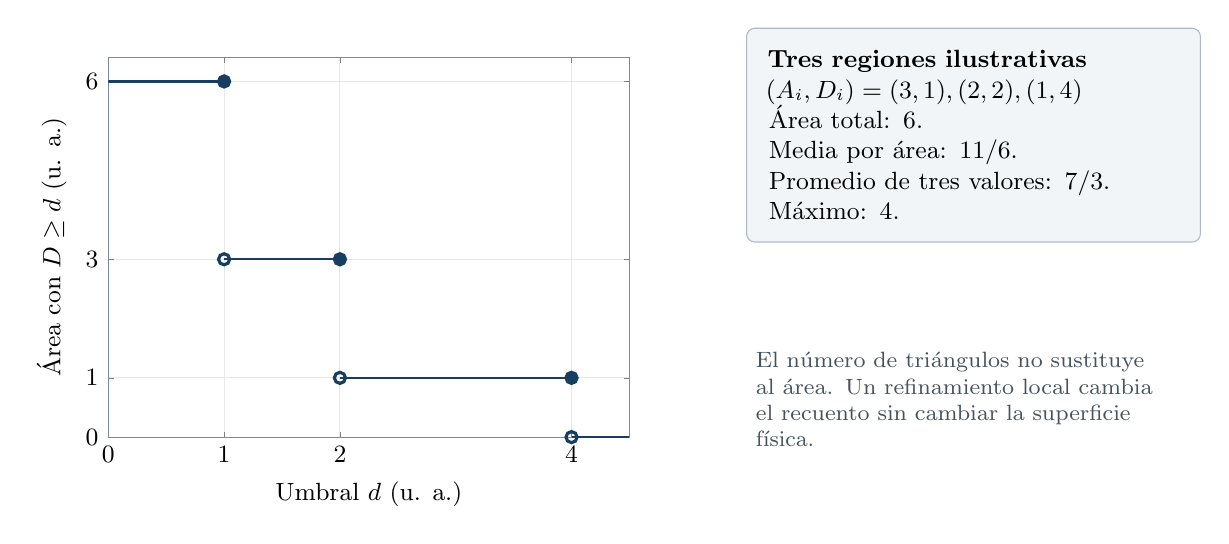
\begin{tikzpicture}[font=\small]
\begin{axis}[dermaplot,width=8.2cm,height=6.4cm,xlabel={Umbral $d$ (u. a.)},ylabel={Área con $D\geq d$ (u. a.)},xmin=0,xmax=4.5,ymin=0,ymax=6.4,xtick={0,1,2,4},ytick={0,1,3,6}]
\addplot[azul,thick]coordinates{(0,6)(1,6)};
\addplot[azul,thick]coordinates{(1,3)(2,3)};
\addplot[azul,thick]coordinates{(2,1)(4,1)};
\addplot[azul,thick]coordinates{(4,0)(4.5,0)};
\addplot[only marks,mark=*,azul]coordinates{(1,6)(2,3)(4,1)};
\addplot[only marks,mark=o,azul,mark options={fill=white}]coordinates{(1,3)(2,1)(4,0)};
\end{axis}
\node[panel,text width=5.2cm,anchor=north west]at(8.1,5.2){\textbf{Tres regiones ilustrativas}\\$(A_i,D_i)=(3,1),(2,2),(1,4)$\\Área total: $6$.\\Media por área: $11/6$.\\Promedio de tres valores: $7/3$.\\Máximo: $4$.};
\node[nota,text width=5.2cm,anchor=north west]at(8.1,1.2){El número de triángulos no sustituye al área. Un refinamiento local cambia el recuento sin cambiar la superficie física.};
\end{tikzpicture}

\caption{Histograma acumulado dosis--área de un ejemplo adimensional. Los saltos se ponderan con área y el umbral incluye la igualdad. El dibujo no representa una distribución clínica.}\label{fig:metricas}\end{figure}
\FloatBarrier

\section{Convención algebraica auditada}
Para vectores columna, \codigo{primary_then_secondary} implementa $R_y(\alpha)R_x(\beta)$ y \codigo{secondary_then_primary} implementa $R_x(\beta)R_y(\alpha)$. La matriz de la derecha actúa primero sobre el vector. Los nombres no sustituyen esta definición: la correspondencia con rotaciones intrínsecas del soporte debe verificarse con el equipo. No se ha invertido el orden durante la revisión sin evidencia geométrica de la instalación.
La malla se convierte a mm, cambia de base y recibe \codigo{mesh_origin_mm} en su marco local. Posteriormente recibe las inclinaciones del paciente y su colocación respecto a la mesa. La región de refinamiento se interpreta antes de estas últimas transformaciones.

\chapter{Arquitectura, lectura RDSR y trazabilidad}
\section{Separación de responsabilidades}
El paquete separa la lectura de datos, configuración, geometría, factores, cálculo, métricas y presentación. \codigo{rdsr.py} transforma el árbol DICOM en eventos; \codigo{config.py} construye un equipo; \codigo{geometry.py} proyecta el haz; \codigo{raytrace.py} resuelve primera entrada; \codigo{engine.py} aplica la ecuación y acumula. \codigo{surface_factors.py} y \codigo{factor_tables.py} separan datos físicos e interpolación. \codigo{spectral.py} genera tablas sin alterar el conjunto publicado.

La separación facilita probar funciones sin confundir resultados de visualización con resultados numéricos. También permite introducir un nuevo dataset con el mismo formalismo, siempre que declare medio, ejes, geometría y procedencia. La compatibilidad de esquema es un requisito informático; la compatibilidad física necesita un análisis adicional.
\begin{figure}[htbp]\centering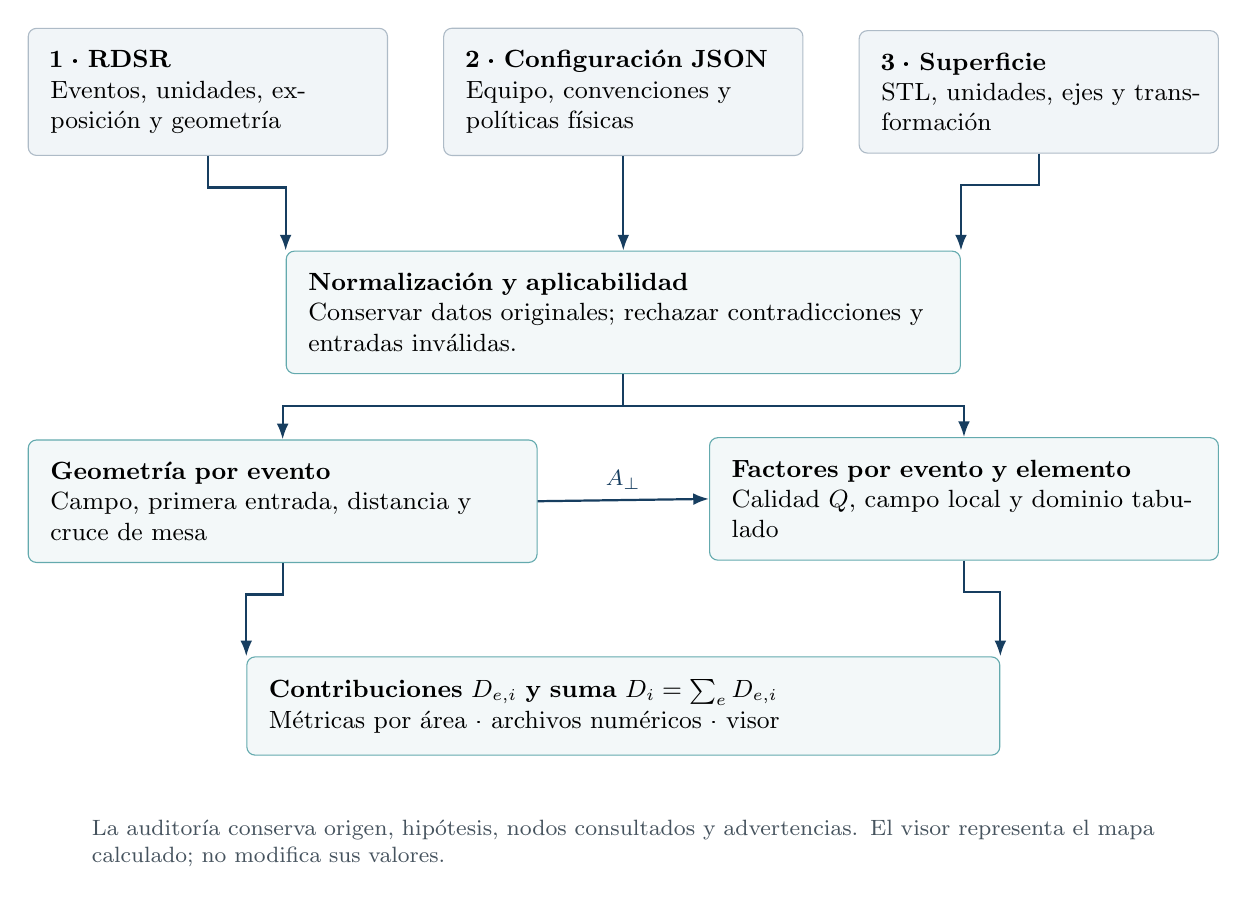
\begin{tikzpicture}[font=\small,node distance=9mm and 7mm]
\node[panel,text width=4cm](r){\textbf{1 · RDSR}\\Eventos, unidades, exposición y geometría};
\node[panel,text width=4cm,right=of r](j){\textbf{2 · Configuración JSON}\\Equipo, convenciones y políticas físicas};
\node[panel,text width=4cm,right=of j](m){\textbf{3 · Superficie}\\STL, unidades, ejes y transformación};
\node[proceso,text width=8cm,below=12mm of j](n){\textbf{Normalización y aplicabilidad}\\Conservar datos originales; rechazar contradicciones y entradas inválidas.};
\draw[flujo](r.south)--++(0,-4mm)-|(n.north west);
\draw[flujo](j)--(n);\draw[flujo](m.south)--++(0,-4mm)-|(n.north east);
\node[proceso,text width=5.9cm,anchor=north west] (g) at ($(r.south west)+(0,-3.6)$){\textbf{Geometría por evento}\\Campo, primera entrada, distancia y cruce de mesa};
\node[proceso,text width=5.9cm,anchor=north east] (q) at ($(m.south east)+(0,-3.6)$){\textbf{Factores por evento y elemento}\\Calidad $Q$, campo local y dominio tabulado};
\draw[flujo](n.south)--++(0,-4mm)-|(g.north);\draw[flujo](n.south)--++(0,-4mm)-|(q.north);\draw[flujo](g.east)--(q.west)node[midway,above,font=\footnotesize]{$A_\perp$};
\node[proceso,text width=9cm,below=12mm of $(g.south)!.5!(q.south)$](d){\textbf{Contribuciones $D_{e,i}$ y suma $D_i=\sum_eD_{e,i}$}\\Métricas por área · archivos numéricos · visor};
\draw[flujo](g.south)--++(0,-4mm)-|(d.north west);\draw[flujo](q.south)--++(0,-4mm)-|(d.north east);
\node[nota,text width=13.5cm,below=7mm of d]{La auditoría conserva origen, hipótesis, nodos consultados y advertencias. El visor representa el mapa calculado; no modifica sus valores.};
\end{tikzpicture}

\caption{Flujo de información de DermaDose. La trazabilidad acompaña a las etapas de cálculo y no se limita a una anotación final.}\end{figure}

\section{Contenido de un evento y normalización}
El lector identifica conceptos por pareja de esquema de codificación y código, en lugar de depender de una cadena descriptiva traducida. El estándar DICOM organiza el evento como entidad de información y permite asociar parámetros de exposición y geometría \citep{dicom}. El código disponible implementa un subconjunto de esa estructura, no un verificador completo del estándar ni de todas las jerarquías comerciales.

Cada evento conserva identificador, modo, kerma, producto kerma-área cuando está disponible, kVp, filtración, ángulos, distancias, campo, mesa y datos originales. Las lecturas numéricas se convierten desde unidades UCUM admitidas. Medidas múltiples incompatibles de un mismo concepto no se promedian silenciosamente. Se rechazan números no finitos e identificadores duplicados.

Las distancias SID, SOD y SRP son nombres internos vinculados a los conceptos que el perfil interpreta. En particular, el uso de SOD como distancia foco--isocentro requiere comprobar su semántica y la correspondencia con el equipo. El nombre de una variable no basta para demostrar que una medida DICOM tenga exactamente esa referencia.

Si solo existe un área de campo y se reconstruye un cuadrado equivalente, se debe conservar la hipótesis. Conocer el área no determina el rectángulo real ni la posición de sus bordes. Las dimensiones y el plano al que se refieren afectan tanto a la máscara como al argumento del factor superficial.

\section{Estados de filtración que deben permanecer distintos}
El análisis de Azurion mostró que exigir material en todos los contenedores producía un fallo ante una declaración explícita de filtro no insertado. La corrección distingue tres situaciones:
\begin{enumerate}
\item \emph{No filter} declarado: se asigna ausencia de filtración añadida representada en ese contenedor, con Cu añadido cero y estado específico.
\item Pila de filtros con material y espesor: se conservan por separado Al y Cu, y se suman capas del mismo material cuando procede.
\item Información ausente o insuficiente: se mantiene el estado desconocido y no se sustituye por cero.
\end{enumerate}
Un contenedor ``No filter'' con material o espesor simultáneo, o una combinación contradictoria de declaraciones, produce error controlado. El aluminio no se convierte en cobre equivalente para facilitar una consulta. Una pila de aluminio conocida sin cobre puede representar Cu añadido cero, pero no una filtración total nula.

Cuando mínimo y máximo difieren, el lector rechaza el evento: el intervalo no determina un espesor homogéneo ni un espectro único. En un filtro homogéneo, DICOM permite declarar el mismo valor en ambos extremos. Si solo se proporciona uno, el lector conserva ese valor; su aceptación es una limitación de lectura y no demuestra homogeneidad. El soporte de materiales y códigos está acotado a lo implementado. Esta política sustituye el promedio aritmético anterior, que carecía de justificación espectral \citep{dicomfilters}.



\begin{figure}[htbp]\centering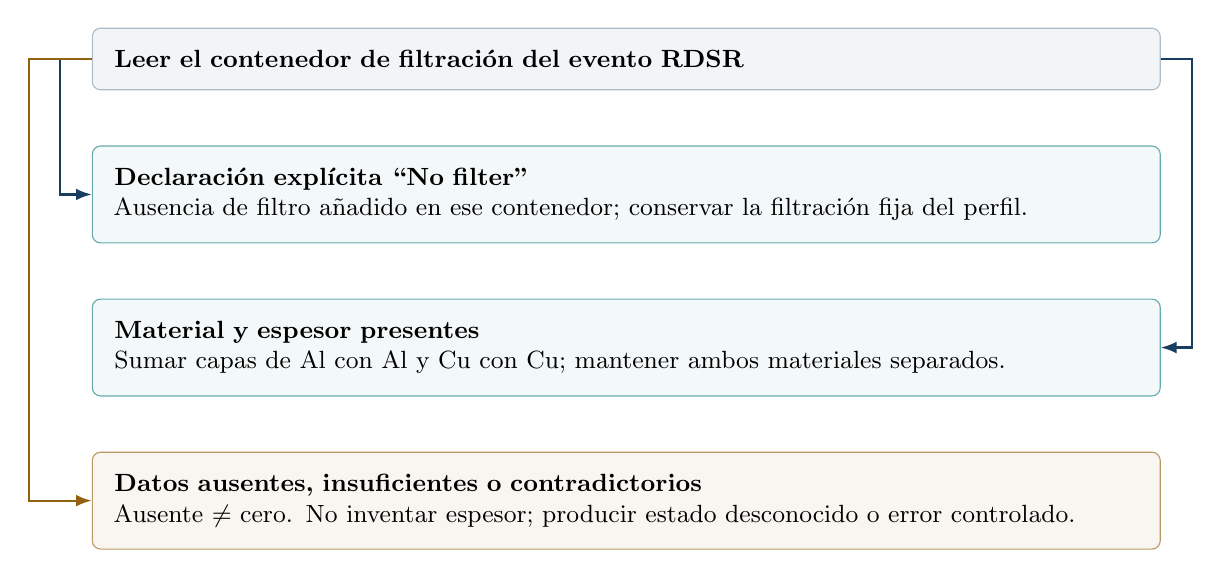
\begin{tikzpicture}[font=\small,node distance=7mm]
\node[panel,text width=13cm](a){\textbf{Leer el contenedor de filtración del evento RDSR}};
\node[proceso,text width=13cm,below=of a](b){\textbf{Declaración explícita ``No filter''}\\Ausencia de filtro añadido en ese contenedor; conservar la filtración fija del perfil.};
\node[proceso,text width=13cm,below=of b](c){\textbf{Material y espesor presentes}\\Sumar capas de Al con Al y Cu con Cu; mantener ambos materiales separados.};
\node[aviso,text width=13cm,below=of c](d){\textbf{Datos ausentes, insuficientes o contradictorios}\\Ausente $\neq$ cero. No inventar espesor; producir estado desconocido o error controlado.};
\draw[flujo](a.west)--++(-4mm,0)|-(b.west);
\draw[flujo](a.east)--++(4mm,0)|-(c.east);
\draw[flujo,ocre](a.west)--++(-8mm,0)|-(d.west);
\end{tikzpicture}

\caption{Estados de información de filtración. Son alternativas de lectura, no etapas consecutivas; el código y las hipótesis del perfil deben conservar su significado.}\label{fig:estados_filtro}\end{figure}

\section{Configuración y control de aplicabilidad}
El JSON de equipo debe incluir versión y bloques coherentes de geometría, paciente y factores. El archivo de metadatos de una exportación de malla no es una configuración completa de DermaDose. El error ``falta version'' observado al usarlo como perfil no se soluciona añadiendo una etiqueta arbitraria: faltan definiciones físicas y geométricas.

Las rutas se resuelven respecto a la configuración. Mover el JSON a una carpeta de ejemplo cambia la relación con la malla y el dataset. Los errores de archivo ausente son problemas de localización, diferentes de un evento fuera de dominio o de una geometría inválida. El anexo ofrece una estructura reproducible que evita depender de la carpeta actual de la terminal.

El perfil Azurion exige indicadores de caracterización cuando no se permiten hipótesis. Marcar esos indicadores a verdadero no realiza una calibración: deben estar respaldados por medidas, identificación del equipo y un registro de su evaluación. En investigación se permiten sustituciones explícitas, registradas en la calidad del evento, que siguen siendo hipótesis.

\section{Caché y acumulación}
La caché conserva proyecciones de geometrías exactamente coincidentes. Reutiliza la selección y magnitudes geométricas, mientras que kerma y factores se recalculan para cada evento. La corrección de la caché se evalúa comparando mapas con la vía sin caché, no únicamente tiempos.

La suma mantiene los índices de una superficie fija. Con $N$ elementos y $E$ eventos, conservar todos los mapas en \codigo{float64} exige al menos $8NE$ bytes, antes de añadir geometría, índices y copias. La implementación actual puede crear matrices apiladas para acumular, con un máximo de memoria superior al almacenamiento base.

La trazabilidad por evento es valiosa para explicar máximos y depurar casos, pero tiene un coste. Una futura acumulación por bloques deberá decidir qué contribuciones conservar, cómo permitir inspección posterior y cómo mantener igualdad numérica dentro de tolerancias justificadas.

\section{Salidas y procedencia}
Las salidas incluyen un informe JSON, matrices de mapa en NPZ, tabla de eventos, figuras, histograma dosis--área y visor HTML. Deben conservar etapa física, medio, factores, geometría, advertencias y huellas de entradas. Los metadatos tabulados registran nodos fuente y si la consulta es exacta o interpolada.

La presencia de un \emph{hash} no acredita que una tabla sea correcta: acredita correspondencia con unos bytes identificados. Su utilidad es detectar modificaciones y permitir repetir el mismo cálculo. La revisión humana de unidades, transcripción y definición física sigue siendo necesaria.

Los informes reales pueden contener identificadores en el árbol SR y en metadatos del archivo. Una revisión de desidentificación debe abarcar ambos y conservar relaciones internas necesarias. Esta memoria presenta solo recuentos agregados del caso de trabajo; no distribuye su DICOM ni identificadores de eventos.


\chapter{Superficie del paciente a partir de TC con 3D Slicer}

\section{Flujo de trabajo actual}
DermaDose utiliza como superficie de entrada el contorno externo del paciente extraído de una TC con el módulo \textit{DermaDose Surface} de 3D Slicer. La ejecución de ejemplos utiliza el STL aportado en la carpeta del caso. XCAT se conserva como referencia histórica para las demostraciones y comparaciones anteriores, pero ha dejado de ser una opción del lanzador de casos. Este cambio permite trabajar con la forma individual de la región irradiada y documentar la procedencia de cada superficie.

La geometría del contorno y su colocación durante la intervención son problemas distintos. Una TC puede representar la forma del paciente en el momento de la adquisición, mientras que el apoyo, la postura de los brazos, la respiración y la posición sobre la mesa pueden cambiar en la sala intervencionista. El contorno externo sirve para localizar la entrada del haz. Para calcular transporte en órganos haría falta representar además la anatomía interna y los materiales.

\section{Extracción y revisión en DermaDose Surface}
La versión \codigo{1.8.0-anclaje-toracico} toma como entrada un volumen de TC seleccionado en 3D Slicer. El procedimiento de trabajo es el siguiente:

\begin{enumerate}
\item Seleccionar el volumen y comprobar que cubre la región intervenida. El umbral inicial de $-350$ HU es orientativo y puede ajustarse a partir de los cortes.
\item Extraer el contorno externo mediante umbralización, selección de la mayor componente con conectividad de seis vecinos y relleno de cavidades internas. Revisar y, si procede, editar el segmento antes de preparar la superficie.
\item Preparar la malla, revisar el resultado de los controles y comprobar visualmente el contorno en los cortes y en la vista 3D. Prestar atención al contacto con la mesa, las extremidades y los extremos del volumen.
\item Exportar el STL y su JSON homónimo después de confirmar la revisión. Conservar ambos archivos juntos para el cálculo.
\end{enumerate}

Las operaciones de extracción y preparación que usan el proceso auxiliar se ejecutan mediante \codigo{PythonSlicer}, con indicación de progreso en la interfaz. Esto separa el trabajo pesado de la interacción con la ventana de Slicer. La edición del segmento y la revisión de la superficie siguen siendo parte del flujo.

\begin{figure}[htbp]\centering\begin{tikzpicture}[font=\small,node distance=7mm and 8mm]
\node[panel,text width=4cm](a){\textbf{1 · Seleccionar TC}\\HU, cobertura, espaciado y ejes};
\node[proceso,text width=4cm,right=of a](b){\textbf{2 · Contorno binario}\\Umbral inicial $-350$ HU; mayor componente; relleno};
\node[proceso,text width=4cm,right=of b](c){\textbf{3 · Superficie original}\\Limpieza, orientación y comprobación};
\draw[flujo](a)--(b);\draw[flujo](b)--(c);
\node[proceso,text width=4cm,below=12mm of c](d){\textbf{4 · Intentar simplificación}\\Objetivo: \num{150000} caras; preservar topología};
\draw[flujo](c)--(d);
\node[aviso,text width=4cm,left=of d](e){\textbf{5 · ¿Reducción válida?}\\Cierre, conectividad, degeneración y volumen};
\draw[flujo](d)--(e);
\node[proceso,text width=4cm,left=of e](v){\textbf{Sí: malla reducida}\\No: conservar original válida con aviso};
\draw[flujo](e)--(v);
\node[panel,text width=12.8cm,below=12mm of e](out){\textbf{6 · Revisión visual y exportación}\\STL + JSON de metadatos (RAS, mm, caras reales); lectura de comprobación antes de confirmar.};
\draw[flujo](v.south)--++(0,-5mm)-|(out.north west);
\node[nota,text width=13cm,below=6mm of out]{Un contorno cerrado puede estar truncado, incluir mesa o excluir una extremidad. La validez topológica no demuestra fidelidad anatómica.};
\end{tikzpicture}

\caption{Preparación y exportación del contorno del paciente en DermaDose Surface. La reducción está subordinada a los controles geométricos y a la revisión visual.}\end{figure}

\section{Simplificación, controles y exportación}
El objetivo inicial es de \num{150000} caras. El módulo ofrece preparación con un intervalo de \num{100000} a \num{200000} caras y un modo de velocidad que puede probar un objetivo mayor cuando el primero falla. También permite exportar un par de superficies con objetivos de \num{150000} y \num{300000} caras para estudiar la sensibilidad a la resolución. Si una superficie ya tiene menos caras, se conserva sin subdividirla artificialmente. Si la preparación no admite una reducción, el original queda disponible para revisión y la exportación reducida se bloquea.

Se comprueban coordenadas finitas, degeneración, componentes, bordes abiertos, aristas no manifold y volumen. La simplificación se somete a controles de conservación geométrica. Antes de publicar la pareja de archivos se relee el STL temporal para verificar la geometría exportada. Los archivos se crean sin sobrescribir una pareja existente. Un contorno cerrado puede estar truncado, incluir parte del tablero o excluir una extremidad; por eso la inspección visual sigue siendo necesaria.

\section{Metadatos y colocación respecto al angiógrafo}
El STL se exporta en milímetros y coordenadas RAS. El JSON de superficie documenta, entre otros datos, el nombre y el hash del STL, la transformación de índices de vóxel a RAS, el umbral, el resultado de la reducción y los controles de geometría. El módulo intenta extraer un anclaje torácico estimado a partir de dos regiones pulmonares plausibles cuando la TC lo permite. Esta referencia es opcional y queda identificada en el JSON.

La carpeta de cálculo contiene el RDSR, el STL, su JSON de Slicer y un único JSON de equipo. El primero aporta los eventos de irradiación; el segundo y su archivo asociado describen la superficie; el perfil de equipo aporta la geometría de sala y el modelo dosimétrico. El lanzador selecciona el STL del caso y puede estimar la transformación con la postura registrada en el RDSR, la geometría de mesa y un evento de referencia. Si existe un anclaje compatible con la región del estudio, lo utiliza. En su ausencia puede recurrir al centro de los límites de la malla como aproximación. La configuración efectiva y la procedencia del anclaje se guardan con los resultados.

La colocación obtenida es una estimación. Antes de interpretar la localización de la dosis se deben comprobar lateralidad, sentido cabeza--pies, apoyo y cobertura de la región irradiada. El motor de dosis se ejecuta fuera de Slicer y la exportación del STL y sus metadatos constituye la interfaz entre ambos.

\section{Rendimiento y elección de resolución}
Reducir caras puede disminuir preparación geométrica, candidatos de intersección, mapas y tamaño del HTML. No garantiza una disminución proporcional del tiempo total, porque pueden dominar consultas al índice, métricas locales o exportación. La interacción entre tamaño de caras y número de rayos debe medirse en una carga representativa.

La selección de resolución debería basarse en diferencias de PSD, posición del máximo, áreas e integral entre representaciones. Si la simplificación desplaza la superficie, también se modifica la distancia física del cálculo. En cambio, refinar un triángulo plano solo cambia los puntos de muestreo. Confundir estas operaciones puede atribuir al rendimiento un cambio dosimétrico que procede de anatomía alterada.
\FloatBarrier

\section{Justificación del tamaño de los elementos}
Se propone, como criterio inicial de investigación, una longitud característica de aproximadamente 5 mm y un objetivo de exportación de \num{150000}--\num{200000} caras para una superficie de cuerpo completo. El objetivo combina fidelidad geométrica, muestreo dosimétrico y coste computacional; no es un requisito normativo ni una resolución clínicamente validada. El número total no garantiza el tamaño local: deben registrarse distribuciones de áreas y longitudes de arista, además de la forma de los triángulos.

Para triángulos aproximadamente equiláteros de lado $h$ sobre una superficie de área $S$, la estimación $N\simeq4S/(\sqrt{3}h^2)$ permite relacionar resolución y número de caras. Tomando $S=1{,}8$ m$^2$ únicamente como ejemplo, $h=5$ mm requiere unas \num{166000} caras, frente a \num{462000} para 3 mm y \num{1040000} para 2 mm. Una segmentación anatómica parcial necesita menos caras para una misma resolución. Por tanto, \num{150000} caras representan un presupuesto inicial, no una garantía universal de suficiencia.

La evaluación por cara hace especialmente sensibles los bordes de campo y los solapamientos estrechos: el centro de una cara parcialmente irradiada puede no representar su fracción realmente expuesta. Se propone comprobar los máximos mediante refinamiento local a 2--3 mm en regiones irradiadas, incluyendo sus bordes. En el ejemplo regular, un área de 1 cm$^2$ contiene unas nueve caras de lado 5 mm y unas 26 de lado 3 mm; aumentar ese muestreo mejora la descripción discreta, sin convertir la vecindad implementada en un dosímetro exacto de 1 cm$^2$. La bibliografía describe el beneficio de refinar para delimitar el haz; ello no establece una resolución obligatoria para DermaDose.

El coste crece al aumentar muestras, intersecciones y vecindades. Solo almacenar un valor de doble precisión por cara y evento exige $8NE$ bytes: para 101 eventos, unas \num{150000} caras requieren 121 MB y un millón, 808 MB, sin contar geometría, cachés, copias o visor. No se asignan tiempos concretos sin medirlos en el equipo de ejecución.

La selección definitiva debe basarse en convergencia con anatomía fija: comparar, por ejemplo, 7, 5, 3 y 2 mm, evaluando PSD puntual, máximo promediado sobre 1 cm$^2$, región de alta dosis, tiempo y memoria. Una variación inferior al 2--3\,\% entre refinamientos sucesivos puede utilizarse como objetivo interno inicial, explícitamente propuesto y no como tolerancia clínica publicada. La fidelidad de la simplificación debe comprobarse por separado frente a la superficie original: subdividir caras no recupera anatomía perdida. Estas decisiones tampoco sustituyen la caracterización del equipo, el registro anatómico o la validación dosimétrica externa.

\chapter{Factores de Benmakhlouf: definición y uso}
\section{Fuente de los datos y geometría original}
La fuente directa del dataset es el informe KS-ASF-201101-IR de Benmakhlouf, Fransson y Andreo, de 7 de abril de 2011 \citep{benreport}. Se distingue del artículo de revista asociado, que incluye un autor adicional \citep{benarticle}. Los valores del programa deben atribuirse a la tabla concreta del informe, no a una referencia genérica sin localización.

Los autores calcularon respuestas monoenergéticas con PENELOPE 2008 y PenEasy. La sección de métodos describe una base de 44 energías entre 4 y 150 keV; la tabla 1 imprime 30 nodos de 5 a 150 keV en incrementos de 5 keV. DermaDose conserva esos 30 nodos publicados y no reconstruye los valores no impresos.

La geometría utiliza entrada plana de agua, espesor de 15 cm, distancia foco--superficie de 100 cm y campos cuadrados de lados 5, 10, 20, 25 y 35 cm. La fluencia se evalúa en una región central de $1\times1\times\num{0.01}$ cm$^3$. El transporte electrónico detallado se desactiva para estos cálculos de kerma, suponiendo depósito local; el corte de transporte fotónico se fija en 1 keV. Son condiciones del cálculo original, no parámetros ejecutados por el motor de malla.

Las especificaciones laterales discordantes del informe se conservan en los metadatos. Para una reproducción independiente habría que aclarar la geometría efectivamente utilizada para los campos mayores. No se debe inferir una resolución de esa discrepancia a partir de que el CSV sea legible.

\section{Factor de retrodispersión en aire}
Se denota por $\Phi^{\mathrm{prim}}_Q(E)$ el espectro incidente y por $\Phi^{\mathrm{sup}}_{Q,s}(E)$ el total superficial, que incorpora primarios y retrodispersados. El factor utilizado por el formalismo es
\begin{equation}\label{eq:bs}
B(Q,s)=\frac{\int E\Phi^{\mathrm{sup}}_{Q,s}(E)\muen{\mathrm{aire}}(E)\,\mathrm dE}
{\int E\Phi^{\mathrm{prim}}_Q(E)\muen{\mathrm{aire}}(E)\,\mathrm dE}.
\end{equation}
El numerador corresponde al kerma evaluado en aire en la superficie del fantoma de agua. La palabra ``aire'' identifica la magnitud y su coeficiente, no la ausencia de fantoma en el numerador. El denominador es el haz primario libre en aire en el mismo plano.

El factor depende de calidad y campo, así como de las condiciones del fantoma. El informe proporciona una respuesta central. Aplicarlo uniformemente a cada punto local de una anatomía curva no reproduce de manera explícita la reducción de dispersión cerca de un borde ni la respuesta de materiales internos distintos.

\section{Conversión superficial agua--aire}
La conversión de medio correspondiente al espectro superficial puede escribirse como
\begin{equation}\label{eq:ratio}
f(Q,s)=\frac{\int E\Phi^{\mathrm{sup}}_{Q,s}(E)\muen{\mathrm{agua}}(E)\,\mathrm dE}
{\int E\Phi^{\mathrm{sup}}_{Q,s}(E)\muen{\mathrm{aire}}(E)\,\mathrm dE}.
\end{equation}
No es simplemente el cociente de coeficientes en una energía media. Para un haz incidente monoenergético de energía $E_0$, la radiación retrodispersada contiene otras energías; por eso el valor publicado $f(E_0,s)$ conserva una dependencia con el campo.

El producto $Bf$ convierte el kerma primario en aire a una magnitud superficial de agua bajo las hipótesis del informe. La transferencia a ``piel'' debe mantener esa referencia material. El programa exige aceptar explícitamente la aproximación de fantoma de agua y declarar la base de kerma incidente para reducir el riesgo de doble conteo.


La figura~\ref{fig:monoenergeticos} permite distinguir la respuesta monoenergética del espectro clínico: la energía del eje identifica el haz primario de cada cálculo original. No representa las energías de todos los fotones que retornan a la superficie.
\begin{figure}[p]\centering\begin{tikzpicture}
\begin{axis}[dermaplot,name=mono,height=6.2cm,title={A · Retrodispersión en aire},xlabel={Energía incidente monoenergética (keV)},ylabel={$B(E,s)$},xmin=5,xmax=150,legend style={at={(.98,.98)},anchor=north east}]
\addplot[azul,solid,mark=*,mark size=.8pt]table[x=energy_kev,y=B,col sep=comma]{datos/mono_s5.csv};
\addlegendentry{$s=5$ cm}
\addplot[turquesa,dashed,mark=*,mark size=.8pt]table[x=energy_kev,y=B,col sep=comma]{datos/mono_s20.csv};
\addlegendentry{$s=20$ cm}
\addplot[ocre,dash dot,mark=*,mark size=.8pt]table[x=energy_kev,y=B,col sep=comma]{datos/mono_s35.csv};
\addlegendentry{$s=35$ cm}
\end{axis}
\begin{axis}[dermaplot,at={(mono.below south west)},anchor=north west,yshift=-1.25cm,height=6.2cm,title={B · Corrección combinada superficial},xlabel={Energía incidente monoenergética (keV)},ylabel={$C(E,s)$},xmin=5,xmax=150,legend style={at={(.98,.98)},anchor=north east}]
\addplot[azul,solid,mark=*,mark size=.8pt]table[x=energy_kev,y=C,col sep=comma]{datos/mono_s5.csv};
\addplot[turquesa,dashed,mark=*,mark size=.8pt]table[x=energy_kev,y=C,col sep=comma]{datos/mono_s20.csv};
\addplot[ocre,dash dot,mark=*,mark size=.8pt]table[x=energy_kev,y=C,col sep=comma]{datos/mono_s35.csv};
\end{axis}
\end{tikzpicture}

\caption{Factores monoenergéticos de tres campos: $B$ tabulado y producto nodal $C=Bf$. Datos de la tabla 1 del informe de Benmakhlouf, conservados en los CSV del proyecto. Los puntos son nodos publicados; los segmentos guían la lectura. No son factores medidos del Azurion.}\label{fig:monoenergeticos}\end{figure}

\section{Tres integraciones que no deben confundirse}
La ecuación 11 del informe promedia $B(E,s)$ con pesos de kerma primario en aire:
\begin{equation}\label{eq:meanB}
B(Q,s)=\frac{\int K_a(E;Q)B(E,s)\,\mathrm dE}{\int K_a(E;Q)\,\mathrm dE},
\qquad K_a(E;Q)\propto E\Phi_Q(E)\muen{\mathrm{aire}}(E).
\end{equation}
Su ecuación 12 prescribe para el cociente tabulado un promedio con fluencia energética del primario,
\begin{equation}\label{eq:eq12}
f_{\mathrm{ec.12}}(Q,s)=\frac{\int E\Phi_Q(E) f(E,s)\,\mathrm dE}{\int E\Phi_Q(E)\,\mathrm dE},
\end{equation}
donde $f(E,s)$ ya incorpora la respuesta superficial obtenida para cada irradiación monoenergética. Debe respetarse esa definición al discutir la construcción de las filas clínicas originales.

Para una corrección combinada, el informe ofrece la ecuación 13:
\begin{equation}\label{eq:eq13}
C(Q,s)=\frac{\int K_a(E;Q)C(E,s)\,\mathrm dE}{\int K_a(E;Q)\,\mathrm dE},
\qquad C(E,s)=B(E,s)f(E,s).
\end{equation}
La ampliación espectral del proyecto implementa esta última vía. No calcula un promedio independiente de $B$ y otro de $f$ para multiplicarlos posteriormente como sustitución de la ecuación~\eqref{eq:eq13}.

En general, para pesos comunes $w$, $\langle Bf\rangle_w\neq\langle B\rangle_w\langle f\rangle_w$; su diferencia es una covarianza ponderada. Además, la ecuación~\eqref{eq:eq12} utiliza pesos distintos. Por ello no debe exigirse identidad exacta entre la nueva corrección combinada y el producto de dos factores clínicos redondeados obtenidos por el otro procedimiento.

\section{Tablas clínicas publicadas y su dominio}
Las filas clínicas del informe se obtuvieron mediante espectros de tungsteno generados con SpekCalc. Cubren kVp de 50 a 150 y las cinco dimensiones de campo. Se organizan por familias discretas de Al de \num{2.5}, \num{3.1}, \num{4.1} y \num{5.1} mm, con dominios de Cu distintos.
\begin{table}[htbp]\centering
\caption{Nodos de cobre añadido del dataset clínico original para cada familia de Al.}
\begin{tabular}{ll}\toprule
Al de la familia (mm) & Cu añadido (mm)\\\midrule
\num{2.5} & 0; \num{0.3}; \num{0.9}\\
\num{3.1} & 0; \num{0.1}; \num{0.2}; \num{0.3}; \num{0.6}; \num{0.9}\\
\num{4.1} & 0; \num{0.1}; \num{0.2}\\
\num{5.1} & 0\\\bottomrule
\end{tabular}
\fuente{CSV clínico del proyecto, contrastado con tabla 3 del informe. Un intervalo permite interpolación únicamente dentro de la familia elegida.}
\end{table}
La familia de \num{4.1} mm Al no permite \num{0.4} mm Cu, aunque exista una fila con mayor Cu en otra familia. No se debe trasladar la consulta a otra fila de aluminio sin justificar el espectro. Tampoco es correcto reemplazar Cu por un espesor de Al equivalente fijo para todas las energías.



\begin{figure}[htbp]\centering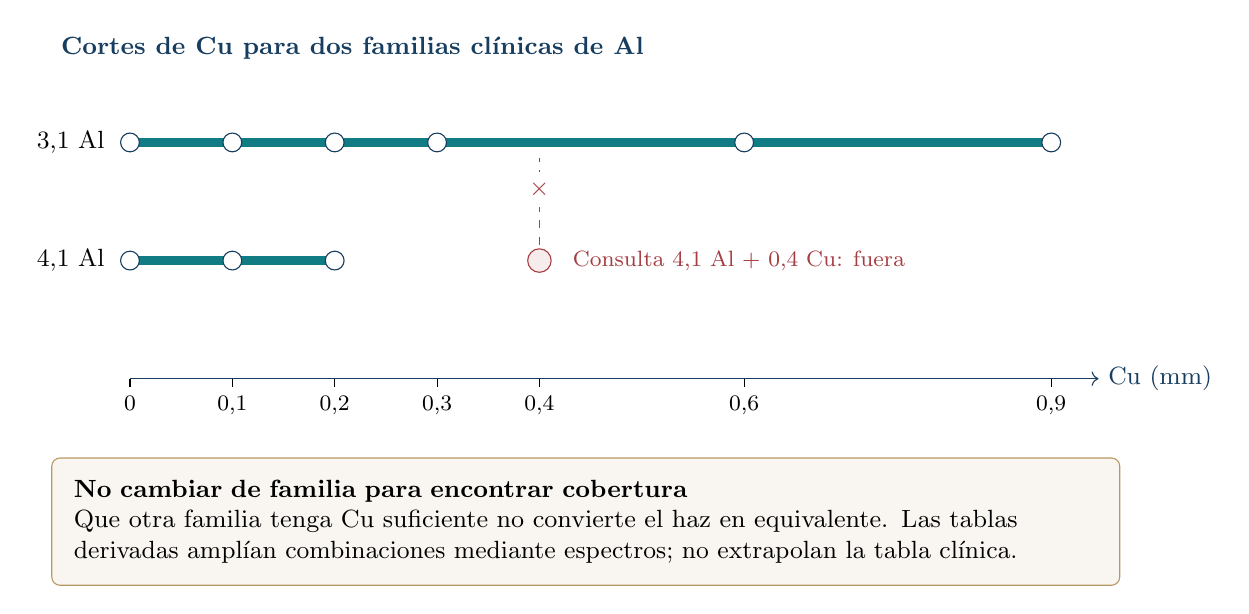
\begin{tikzpicture}[font=\small,x=1cm,y=1cm]
\node[rotulo,anchor=west]at(0,4.2){Cortes de Cu para dos familias clínicas de Al};
\draw[->,azul](1,0)--(13.3,0)node[right]{Cu (mm)};
\foreach \v/\lab in {0/0,1/{0,1},2/{0,2},3/{0,3},4/{0,4},6/{0,6},9/{0,9}}{
\draw(1+1.3*\v,0)--++(0,-.1);\node[below,font=\footnotesize]at(1+1.3*\v,-.1){\lab};}
\node[anchor=east]at(.8,3){$3{,}1$ Al};\node[anchor=east]at(.8,1.5){$4{,}1$ Al};
\draw[turquesa,line width=3pt](1,3)--(12.7,3);\draw[turquesa,line width=3pt](1,1.5)--(3.6,1.5);
\foreach \v in {0,1,2,3,6,9}\node[circle,draw=azul,fill=white,inner sep=2.4pt]at(1+1.3*\v,3){};
\foreach \v in {0,1,2}\node[circle,draw=azul,fill=white,inner sep=2.4pt]at(1+1.3*\v,1.5){};
\node[circle,draw=rojo,fill=rojo!10,inner sep=3pt]at(6.2,1.5){};
\node[nota,anchor=west,text=rojo]at(6.5,1.5){Consulta $4{,}1$ Al + $0{,}4$ Cu: fuera};
\draw[rojo,dashed](6.2,1.7)--(6.2,2.8);\node[text=rojo,fill=white]at(6.2,2.4){$\times$};
\node[aviso,text width=13cm,anchor=north west]at(0,-1){\textbf{No cambiar de familia para encontrar cobertura}\\Que otra familia tenga Cu suficiente no convierte el haz en equivalente. Las tablas derivadas amplían combinaciones mediante espectros; no extrapolan la tabla clínica.};
\end{tikzpicture}

\caption{Dominio de Cu dentro de familias discretas de Al del dataset clínico original. Círculos: nodos publicados; segmentos: interpolación admitida en Cu con el resto de ejes compatibles. No se interpola entre familias de Al.}\label{fig:dominio}\end{figure}

\section{Interpolación y conservación de procedencia}
Las tablas completas se interpolan de forma multilineal y se rechazan consultas exteriores. En un eje, $F(x)=(1-\lambda)F_0+\lambda F_1$, con $\lambda=(x-x_0)/(x_1-x_0)$. En varios ejes se combinan los pesos de las esquinas. Un nodo exacto conserva el valor original.

El proveedor clínico interpola $B$ y $f$ por separado en kVp, Cu y lado; no interpola entre familias de Al. La base monoenergética interpola energía y lado dentro de sus límites. La generación de $C(E,s)$ introduce una decisión específica: primero calcula el producto en los nodos impresos y luego interpola ese producto. Multiplicar dos interpolantes sería un procedimiento distinto entre nodos.

Se comprueban número de filas, ausencia de duplicados, positividad, finitud, malla cartesiana completa y SHA-256. El informe de consulta conserva filas fuente y estado de interpolación. Las cifras anómalas o advertencias del origen se propagan como metadatos; no se corrigen silenciosamente para embellecer la tabla. En concreto, la transcripción conserva valores impresos del descriptor $h$ mayores que uno en 24 calidades de la familia Al de 3,1 mm y kVp de 120--150. Se marcan como observación de fuente y ese descriptor no se utiliza en la interpolación dosimétrica. No se reinterpretan como nuevas medidas de HVL ni se usan para ajustar el espectro.

\section{Agua, forma del campo y límites de transferencia}
Para un rectángulo, la opción \codigo{equal_area} utiliza $s=\sqrt{A_\perp}$. Es una aproximación de igual área. No es equivalente a un cuadrado de Sterling $2ab/(a+b)$ ni garantiza igual retrodispersión en campos alargados. La política \codigo{square_only} rechaza esa sustitución si no se acepta explícitamente.

Los límites de 5--35 cm se refieren al lado del campo normal al eje en el plano de entrada. Un cambio de profundidad local puede hacer que una consulta salga del intervalo aun cuando el campo nominal en detector sea admisible. El control debe ejercerse en la superficie realmente evaluada.

El conjunto no cubre de manera independiente espesor anatómico, hueso, curvatura, incidencia oblicua o posiciones fuera del eje. Su aplicación a XCAT conserva esas aproximaciones incluso si todas las coordenadas numéricas quedan dentro de los ejes de la tabla. Estar dentro del dominio de interpolación es necesario, pero no suficiente para establecer validez física.
\FloatBarrier

\chapter{Adaptación de investigación a Philips Azurion}
\section{Identidad del equipo y alcance del perfil}
El trabajo reciente utiliza un RDSR que declara fabricante Philips y modelo Azurion. El perfil incorpora controles de identidad y políticas específicas de lectura y configuración. Esto permite trabajar con las particularidades observadas sin cambiar el informe original ni extender una suposición a cualquier equipo de la misma marca.

La denominación Azurion identifica una familia, no un único espectro. La instalación puede diferir por tubo, configuración de limitador, versión, mantenimiento y programa clínico. Para construir un perfil físico se necesita identificar esos elementos. Una configuración denominada ``Azurion'' que conserva factores sintéticos sigue siendo de investigación.

\section{Qué aporta la documentación del fabricante}
La documentación oficial consultada para Release 1.2 describe una filtración mínima del conjunto tubo--carcasa equivalente a \num{2.5} mm Al. También identifica filtros añadidos de \num{0.1}, \num{0.4} y \num{0.9} mm Cu, cada uno con 1 mm Al, para el limitador de haz especificado \citep{philipsifu}. La nota 41 del documento ClarityIQ confirma la presencia del aluminio acompañante al cobre \citep{clarity}.

Esta información fundamenta conservar ambos materiales. No determina la filtración fija efectiva total de la instalación ni justifica por sí sola \num{3.1} mm Al. Los espesores equivalentes se refieren a condiciones de calidad del haz declaradas; no representan una equivalencia espectral universal. La versión y el limitador descritos deben contrastarse con los de la sala.

Por tanto, el parámetro de \num{3.1} mm Al de la configuración se clasifica como hipótesis. El ángulo de $12^\circ$ pertenece exclusivamente al dataset histórico. Para el MRC 200 0407 identificado se documentan $11^\circ$; véase el capítulo de caracterización actualizado. El blanco de tungsteno es parte del modelo espectral utilizado y requiere esa misma coherencia de identificación.

\section{Inventario del RDSR de trabajo}
La inspección agregada repetida para esta edición obtiene 101 eventos y tres grupos de filtración añadida. La tabla~\ref{tab:groups} no contiene datos identificativos del procedimiento ni pretende representar la frecuencia de uso del equipo en general.
\begin{table}[htbp]\centering
\caption{Filtración añadida observada en el RDSR de trabajo.}\label{tab:groups}
\begin{tabular}{lrrr}\toprule
Estado & Al añadido (mm) & Cu añadido (mm) & Eventos\\\midrule
Filtro no insertado, explícito & 0 & 0 & 30\\
Pila Al + Cu & 1 & \num{0.1} & 47\\
Pila Al + Cu & 1 & \num{0.4} & 24\\\midrule
Total & & & 101\\\bottomrule
\end{tabular}
\fuente{Inspección de \codigo{0_anon.dcm} mediante \codigo{inspect_azurion}; salida agregada conservada, sin exportar el DICOM.}
\end{table}

El error original ``material filtrante indeterminado'' no demostraba que el tubo careciera de aluminio. Se producía al tratar una declaración de filtro no insertado como si siempre debiera contener material y espesor. La corrección de lectura resuelve esa condición, manteniendo desconocido un filtro realmente no informado.

Hay un evento con kerma no nulo y las tres distancias SID, SOD y SRP nulas. Una distancia cero no permite aplicar el modelo geométrico. No se puede deducir la geometría de ese evento únicamente porque los anteriores tengan valores válidos o porque pertenezca a la misma sala. La sustitución por un valor típico necesita declararse como hipótesis.

\section{Mapeo de aluminio fijo y añadido}
La política \codigo{fixed_plus_event} selecciona una familia según
\begin{equation}\label{eq:al}
a_{\mathrm{total},e}=a_{\mathrm{fijo}}+a_{\text{añadido},e},\qquad
c_e=c_{\text{añadido},e}.
\end{equation}
Con la hipótesis $a_{\mathrm{fijo}}=\num{3.1}$ mm, los eventos explícitamente sin filtro añadido utilizan \num{3.1} mm Al y 0 Cu; los demás utilizan \num{4.1} mm Al y conservan su cobre. El audit registra los tres valores de aluminio: fijo, añadido y familia elegida.
\begin{figure}[htbp]\centering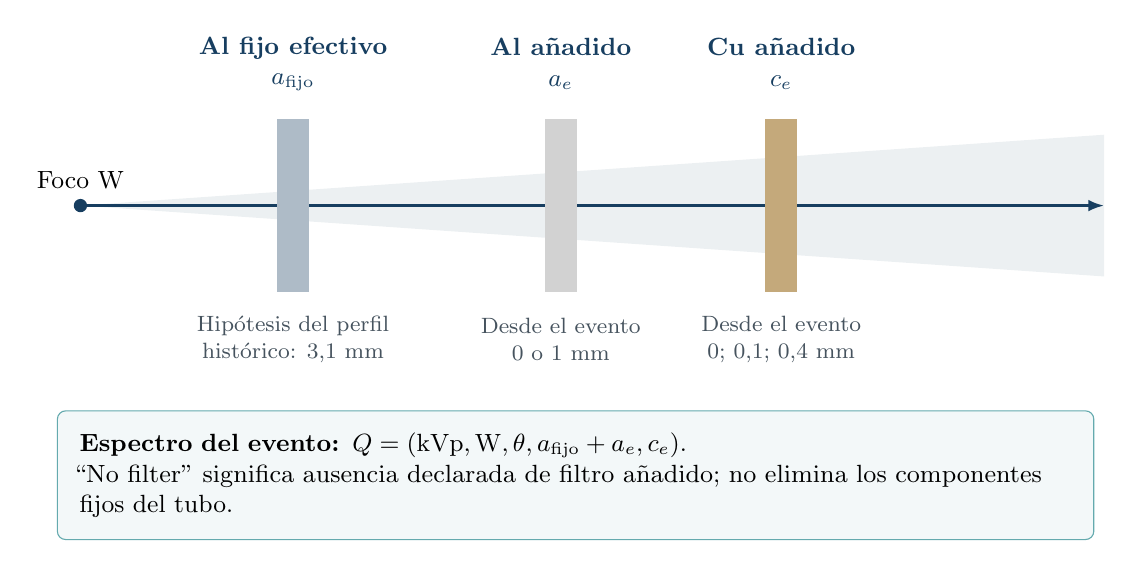
\begin{tikzpicture}[font=\small,x=1cm,y=1cm]
\node[punto,label=above:{Foco W}]at(.5,1.2){};
\fill[azul!8](.5,1.2)--(13.5,2.1)--(13.5,.3)--cycle;
\draw[rayo](.5,1.2)--(13.5,1.2);
\fill[azul!35](3,.1)rectangle(3.4,2.3);
\fill[gray!35](6.4,.1)rectangle(6.8,2.3);
\fill[ocre!55](9.2,.1)rectangle(9.6,2.3);
\node[rotulo,align=center]at(3.2,3){Al fijo efectivo\\$a_{\rm fijo}$};
\node[rotulo,align=center]at(6.6,3){Al añadido\\$a_e$};
\node[rotulo,align=center]at(9.4,3){Cu añadido\\$c_e$};
\node[nota,align=center]at(3.2,-.5){Hipótesis del perfil\\histórico: $3{,}1$ mm};
\node[nota,align=center]at(6.6,-.5){Desde el evento\\$0$ o $1$ mm};
\node[nota,align=center]at(9.4,-.5){Desde el evento\\$0$; $0{,}1$; $0{,}4$ mm};
\node[proceso,text width=12.6cm,anchor=north west]at(.2,-1.4){\textbf{Espectro del evento:} $Q=(\mathrm{kVp},\mathrm W,\theta,a_{\rm fijo}+a_e,c_e)$.\\``No filter'' significa ausencia declarada de filtro añadido; no elimina los componentes fijos del tubo.};
\end{tikzpicture}

\caption{Construcción de la filtración del espectro de investigación. Los espesores de Al no se convierten a Cu equivalente.}\end{figure}

La clave heredada \codigo{inherent_al_mm} representa bajo esta política la hipótesis de Al fijo efectivo, aunque su nombre sugiera una interpretación más restringida. Es necesario documentarlo para no sumar otra vez componentes ya incluidos. Al generar una fila del dataset, el argumento de Al es el total de esa fila; no se añade de nuevo el Al del evento.

Solo se seleccionan familias presentes, con tolerancia numérica para igualdad de flotantes. No se interpola entre familias ni se modifica una tabla original para alojar una combinación nueva. El proveedor comprueba también kVp, Cu y lado de campo local.

\section{Por qué la tabla clínica era insuficiente}
Los 24 eventos de \num{0.4} mm Cu seleccionan, con la hipótesis anterior, la familia de \num{4.1} mm Al. La tabla clínica original de esa familia termina en \num{0.2} mm Cu. El fallo indica falta de cobertura, no un error aritmético ni una imposibilidad de que ese filtro exista en el equipo.

El RDSR contiene además un evento de 46 kVp, por debajo del límite clínico publicado de 50 kVp. Aunque el eje de filtración se resolviera, ese kVp seguiría fuera de la tabla clínica. El campo local introduce una tercera condición independiente: su lado equivalente debe quedar entre 5 y 35 cm.

Usar constantes históricas en los eventos restantes permitiría obtener un número, pero mezclaría dos modelos físicos y ocultaría un cambio de calidad. La decisión implementada para Azurion es mantener un proveedor espectral derivado con procedencia propia y bloquear lo que aún quede fuera, sin sustitución automática por constantes.

\section{Perfil de investigación y plantilla de caracterización}
La configuración de investigación activa \codigo{allow_research_assumptions}. Utiliza distancias configuradas de 810 mm foco--isocentro, \num{1044.3} mm foco--detector y 660 mm foco--referencia cuando se autoriza reemplazar una distancia ausente o no positiva. Son valores de trabajo, derivados de valores habituales válidos del archivo examinado; no son medidas del evento inválido ni especificaciones universales Azurion.

El perfil conserva las distancias válidas de cada evento. También puede tomar las coordenadas de mesa del primer evento como referencia relativa. Esto permite estudiar cambios respecto al inicio, pero no determina dónde se sitúan cabeza, tronco o pelvis respecto al isocentro. El registro anatómico continúa pendiente.

La plantilla de caracterización no permite esas hipótesis por defecto y exige estados de filtración, geometría y calibración caracterizadas. Su función es hacer visible la preparación necesaria. El cambio de indicadores debe acompañarse de nuevos parámetros y evidencia; una modificación del JSON por sí sola no transforma el modelo de investigación en uno validado.

\section{Alcance real de la compatibilidad conseguida}
Se ha conseguido leer las tres categorías de filtros observadas, seleccionar Al total de forma trazable y disponer de una tabla calculada que incluye sus combinaciones de calidad bajo hipótesis. El perfil detecta fabricante/modelo incompatible y no ignora silenciosamente los errores de dominio.

No se ha demostrado que cualquier RDSR Azurion pueda procesarse sin incidencias. Podrían aparecer materiales no soportados, cuñas, campos fuera de rango, otro limitador, barridos o datos geométricos insuficientes. La tabla histórica de 390 filas no contiene \num{0.9} mm Cu, aunque ese filtro figure entre las opciones documentadas del fabricante: ese dataset se construyó para las calidades de trabajo. La alternativa posterior de 910 filas amplía este eje a 0,9 mm Cu, sin demostrar compatibilidad con toda la familia Azurion.

La respuesta científicamente correcta a la pregunta de si ``ya trabaja con Azurion'' es condicional: hay soporte específico de investigación, con lectura y cálculo ampliados, pero faltan caracterización de instalación, registro y validación independiente. La condición debe acompañar al resultado y no quedar solo en una nota de desarrollo.
\FloatBarrier

\chapter{Generación espectral y construcción de tablas derivadas}
\section{Qué se particulariza y para qué}
El capítulo anterior describe el perfil de equipo. Aquí se desarrolla cómo se obtiene, para cada calidad de haz de ese perfil, el factor que transforma el kerma primario en aire a la altura de la piel en una estimación de dosis superficial en agua. La particularización combina dos elementos: la respuesta monoenergética de Benmakhlouf, que describe la retrodispersión y la conversión agua--aire para distintos tamaños de campo, y el espectro incidente calculado para la tensión y la filtración del equipo \citep{benreport,benarticle,spek2020,spek2021}.

La justificación física es la superposición. Para una geometría fija, las contribuciones al kerma de colisión superficial en agua de los distintos intervalos de energía son aditivas. Si el intervalo $i$ aporta un kerma primario en aire $K_{\mathrm{aire},i}^{p}$, su contribución en agua es $K_{\mathrm{aire},i}^{p}C(E_i,s)$, donde $C(E_i,s)=B(E_i,s)f(E_i,s)$ y $s$ es el lado de campo. Dividir la suma de esas contribuciones por el kerma primario total da el factor efectivo $C(Q,s)$ de la ecuación~\eqref{eq:eq13}. La ponderación se hace por kerma incidente: dos intervalos con el mismo número de fotones pueden transferir distinta energía por unidad de masa al aire.

El procedimiento permite calcular factores para calidades de haz que no figuran como filas clínicas en el informe original, siempre que las energías relevantes y los tamaños de campo estén cubiertos por la base monoenergética. La particularización adapta la calidad del haz; las condiciones de retrodispersión siguen siendo las del fantoma de agua de referencia.

\section{Particularización al tubo MRC 200 0407 del Azurion}
Sí se han calculado tablas específicas bajo la identidad documental MRC 200 0407 ROT-GS1004 aportada para el equipo. El dataset \codigo{derived_mrc200_nominal} contiene 1400 filas calculadas con $11^\circ$, blanco W como aproximación del ánodo aleado, paso de 0,5 keV y tensiones de 46 a 125 kV. El límite de 125 kV corresponde al conjunto; no se adopta la tensión superior del inserto aislado. Su construcción y sensibilidad se detallan en el capítulo de caracterización del tubo.

Se incluyen las familias Al de 2,5 y 2,6 mm para dos escenarios nominales, y de 3,5 y 3,6 mm para eventos que declaren 1 mm Al adicional. Se calculan siete nodos de Cu (0, 0,1, 0,2, 0,3, 0,4, 0,6 y 0,9 mm), diez tensiones (46, 50, 60, 70, 80, 90, 100, 110, 120 y 125 kV) y cinco lados de campo (5, 10, 20, 25 y 35 cm). Los nodos intermedios del modelo no se atribuyen a posiciones físicas nuevas del portafiltros.

El perfil de conjunto usa 2,5 mm Al equivalente mínimo; la contribución inherente de 0,8 mm equivalente y la placa de 1,7 mm ya están incluidas. El escenario de 2,6 mm incorpora aproximadamente la contribución de 0,1 mm Al equivalente de la etiqueta de ejemplo del limitador. Es necesario confirmar el limitador instalado y la calidad de referencia de esas equivalencias \citep{mrcservice,azurion22}. No se añade nuevamente el total equivalente de un filtro a sus espesores materiales.

El perfil vigente \codigo{azurion_benmakhlouf_spekpy.json} selecciona estas tablas con el escenario fijo de \num{2.5} mm Al. El escenario con colimador permanece disponible como variante del conjunto de datos para estudios de sensibilidad. La existencia del dataset no activa su uso en cualquier JSON: la configuración efectiva debe apuntar a él y declarar Al y ángulo coherentes. Se conservan los modelos históricos y el ajuste condicionado previo para comparación; no se reemplazan automáticamente las configuraciones del usuario.

\textbf{Particularización documental no equivale a caracterización completa de la instalación.} Las tablas incorporan datos propios del tipo de tubo, pero no acreditan una filtración efectiva medida, orientación ánodo--cátodo, perfil talón, calibración del indicador ni registro anatómico de la sala. Los datos documentales permiten eliminar supuestos incorrectos y estudiar sensibilidad; no demuestran por sí solos mayor exactitud clínica. Los escenarios nominales no sustituyen automáticamente un ajuste basado en medidas compatibles.

\section{Parámetros del generador y significado del espectro}
La tensión de tubo determina la energía cinética máxima de los electrones incidentes y, con ella, el extremo del espectro continuo de frenado. La interacción con el blanco también da lugar a emisión característica. El material del ánodo, su ángulo y la autoabsorción en el blanco condicionan el espectro que emerge. La filtración posterior modifica su forma porque la transmisión de Al y Cu depende de la energía. SpekPy modela estos procesos para obtener la distribución de fluencia incidente que se utilizará en la ponderación \citep{spek2020,spek2021}.

La función \codigo{generate_spectrum} crea un modelo con blanco W, kVp solicitado, ángulo de ánodo y anchura de bin. Para el MRC 200 0407 se utiliza $11^\circ$ y $\Delta E=\num{0.5}$ keV. El valor de $12^\circ$ corresponde exclusivamente a una configuración histórica de comparación y no caracteriza este tubo. Se aplica filtración de Al total y Cu mediante las herramientas de SpekPy. El espectro se obtiene como fluencia diferencial en energía. La conversión a contribuciones de kerma por bin se realiza en el paso siguiente.

La forma general del efecto de filtros homogéneos sobre el primario puede expresarse, de manera ilustrativa, como
\begin{equation}
\Phi_Q(E)=\Phi_0(E;V,\alpha,W)\exp[-\mu_{\mathrm{Al}}(E)a-\mu_{\mathrm{Cu}}(E)c],
\end{equation}
con unidades de espesor compatibles con los coeficientes. El generador implementa su propio modelo y bases; esta expresión explica la dependencia energética y no pretende sustituir sus cálculos internos. No se modelan en esta fase cuñas espaciales, mesa ni colchoneta.

La normalización absoluta de fluencia no es necesaria para el cociente que define $C$. Multiplicar todo el espectro por una constante positiva cancela numerador y denominador. El kerma absoluto de la contribución procede de $\Ka$, con su calibración, en la ecuación del motor. Se evita así sustituir el indicador real por una salida absoluta no caracterizada del generador.

Cada espectro conserva kVp, Al, Cu, ángulo, versión de SpekPy, modelo físico, paso energético, HVL1, HVL2 y una huella del arreglo de energías, fluencias y coeficientes. El modelo registrado en los archivos es \codigo{spekpy-v2-casim}. El acceso a los coeficientes de absorción de energía del aire utiliza un recurso interno de la versión fijada, por lo que futuras actualizaciones requieren comprobar esa interfaz.

\section{Discretización de la integral}
Para centros de bin $E_i$, fluencia diferencial $\Phi_i$, coeficiente $\muen{\mathrm{aire},i}$ y anchura $\Delta E_i$, se construyen
\begin{equation}\label{eq:weights}
w_i=E_i\Phi_i\muen{\mathrm{aire},i}\Delta E_i,
\qquad \widehat w_i=\frac{w_i}{\sum_j w_j}.
\end{equation}
Las constantes de conversión de energía y masa se cancelan en estos cocientes si se emplea una única convención coherente. La presencia de $\Delta E_i$ es necesaria para una fluencia diferencial. Si el generador entregase una cantidad ya integrada por bin, volver a multiplicar por su anchura sería un error.

La implementación comprueba vectores unidimensionales compatibles, energía positiva y estrictamente creciente, fluencia no negativa, coeficientes y anchuras positivos y datos finitos. Rechaza una suma nula de pesos de kerma de colisión. Estas verificaciones protegen la operación matemática; no garantizan que el espectro represente al equipo.

Se calcula primero el producto $C(E_j,s_k)=B(E_j,s_k)f(E_j,s_k)$ en los nodos originales de la tabla monoenergética. Después se interpola ese producto en energía y lado para evaluar los bins del espectro. El factor combinado y la retrodispersión promediada resultan
\begin{equation}
C(Q,s)\simeq\sum_i\widehat w_i C(E_i,s),\qquad
B(Q,s)\simeq\sum_i\widehat w_i B(E_i,s).
\end{equation}
\begin{figure}[htbp]\centering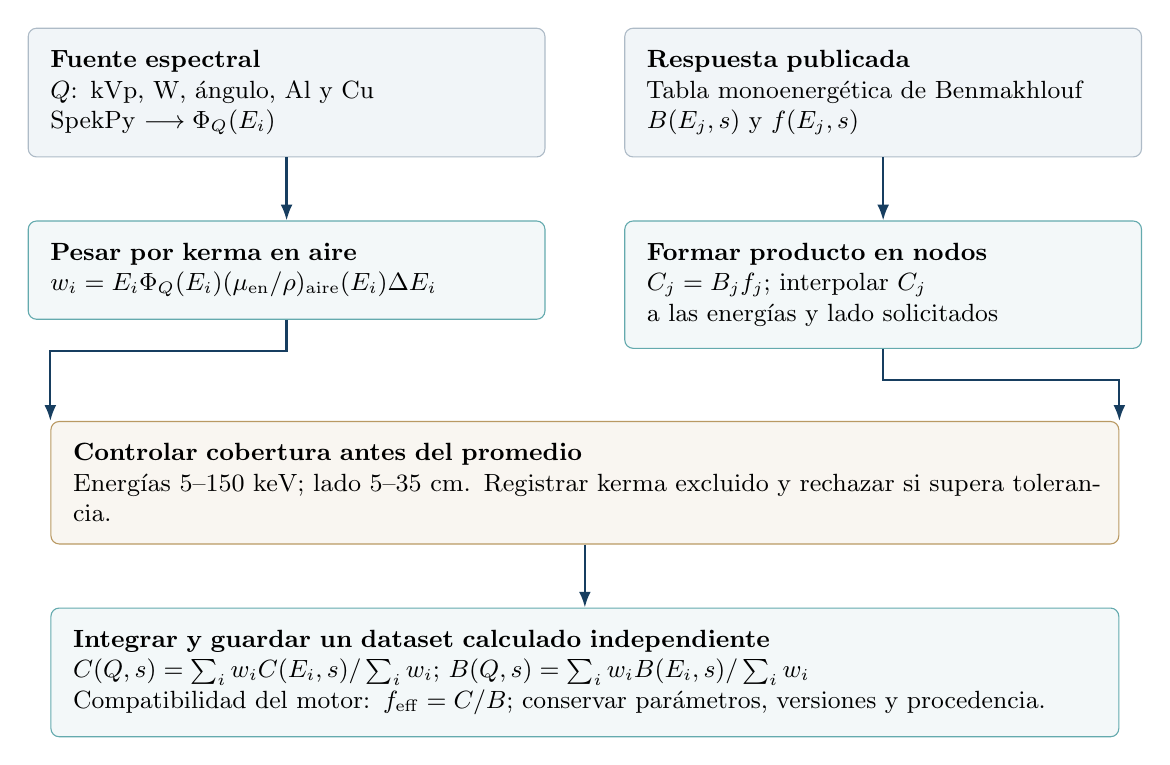
\begin{tikzpicture}[font=\small,node distance=8mm and 10mm]
\node[panel,text width=6cm](a){\textbf{Fuente espectral}\\$Q$: kVp, W, ángulo, Al y Cu\\SpekPy $\longrightarrow\Phi_Q(E_i)$};
\node[panel,text width=6cm,right=of a](b){\textbf{Respuesta publicada}\\Tabla monoenergética de Benmakhlouf\\$B(E_j,s)$ y $f(E_j,s)$};
\node[proceso,text width=6cm,below=of a](w){\textbf{Pesar por kerma en aire}\\$w_i=E_i\Phi_Q(E_i)(\mu_{\rm en}/\rho)_{\rm aire}(E_i)\Delta E_i$};
\node[proceso,text width=6cm,below=of b](c){\textbf{Formar producto en nodos}\\$C_j=B_jf_j$; interpolar $C_j$\\a las energías y lado solicitados};
\draw[flujo](a)--(w);\draw[flujo](b)--(c);
\node[aviso,text width=13cm,below=11mm of $(w.south)!.5!(c.south)$](lim){\textbf{Controlar cobertura antes del promedio}\\Energías 5--150 keV; lado 5--35 cm. Registrar kerma excluido y rechazar si supera tolerancia.};
\draw[flujo](w.south)--++(0,-4mm)-|(lim.north west);\draw[flujo](c.south)--++(0,-4mm)-|(lim.north east);
\node[proceso,text width=13cm,below=of lim](out){\textbf{Integrar y guardar un dataset calculado independiente}\\$C(Q,s)=\sum_iw_iC(E_i,s)/\sum_iw_i$; $B(Q,s)=\sum_iw_iB(E_i,s)/\sum_iw_i$\\Compatibilidad del motor: $f_{\rm eff}=C/B$; conservar parámetros, versiones y procedencia.};
\draw[flujo](lim)--(out);
\end{tikzpicture}

\caption{Construcción del dataset espectral. El promedio se aplica al producto monoenergético y mantiene una procedencia distinta de las filas clínicas publicadas.}\end{figure}

\section{Por qué se almacena un factor efectivo}
El motor espera dos columnas multiplicativas, \codigo{k_bs} y \codigo{k_f}. Para conservar la interfaz sin alterar el factor combinado se define
\begin{equation}\label{eq:feff}
f_{\mathrm{eff}}(Q,s)=\frac{C(Q,s)}{B(Q,s)}.
\end{equation}
Por construcción, $Bf_{\mathrm{eff}}=C$ en cada nodo generado. Este factor efectivo es una descomposición de la corrección conjunta. No debe describirse como la ecuación 12 ni como un nuevo cociente clínico publicado por Benmakhlouf.

Las columnas siguen siendo positivas y compatibles con el producto del motor, pero su interpretación debe acompañar al dataset. Una futura interfaz que admitiese $C$ como magnitud primaria reduciría la ambigüedad de nombres y permitiría controlar de forma directa su interpolación.

Los datasets actuales con metadato \codigo{interpolation_quantity=combined_C} interpolan el producto $C$ directamente, evitando la discrepancia de interpolar $B$ y $f_{\mathrm{eff}}$ por separado. El conjunto MRC 200 0407 declara esa política. Los resultados de interpolación separada del primer dataset se conservan únicamente como análisis de una versión anterior y no describen el proveedor actual.

\section{Dominio energético y truncamiento explícito}
La base impresa cubre 5--150 keV. No se asignan factores inventados a energías inferiores a 5 keV ni superiores a 150 keV. El código calcula la fracción de kerma en los bins exteriores,
\begin{equation}
\varepsilon_{\mathrm{ext}}=\frac{\sum_{i\notin[5,150]}w_i}{\sum_iw_i}.
\end{equation}
La tolerancia explícita de trabajo es $10^{-4}$, equivalente a \num{0.01}\,\% del kerma. Si se supera, se rechaza el espectro. Si se admite la fracción, se integra sobre los bins retenidos y se renormaliza, registrando la exclusión. El API permite tolerancia cero para exigir cobertura completa.

Esta política es una aproximación controlada por kerma excluido, no una demostración de error acotado de $C$ en las energías ausentes: sin conocer su respuesta no puede establecerse una cota universal del sesgo del factor. En los 78 espectros del dataset histórico, la fracción máxima registrada es aproximadamente $6{,}09\times10^{-81}$, despreciable numéricamente en las condiciones generadas.

Incluir 46 kVp es posible porque su espectro se integra con nodos monoenergéticos dentro del dominio permitido. No se extrapola la tabla clínica desde 50 kVp. Esta distinción es una de las ventajas de la vía espectral, aunque sigue dependiendo de la fidelidad del generador para esa calidad.

\section{Diseño de la tabla histórica de comparación}
La malla histórica utiliza 13 tensiones: 46, 50, 60, 70, 80, 90, 100, 110, 120, 125, 130, 140 y 150 kVp. Se combinan dos familias de Al total, \num{3.1} y \num{4.1} mm, con tres de Cu, 0, \num{0.1} y \num{0.4} mm. Para cada una se calculan cinco lados: 5, 10, 20, 25 y 35 cm.
\begin{equation}
N_Q=13\times2\times3=78,\qquad
N_{\mathrm{filas}}=N_Q\times5=390.
\end{equation}
No hay 390 espectros independientes: el mismo espectro de cada calidad se combina con cinco respuestas de campo. Esta separación reduce trabajo y clarifica la procedencia de los factores.

\begin{table}[htbp]\centering\small
\caption{Características del dataset derivado histórico.}
\begin{tabularx}{\textwidth}{p{49mm}Y}\toprule
Propiedad & Valor o condición\\\midrule
Identificador & \codigo{DERIVED-SPEKPY-BENMAKHLOUF-EQ13}\\
Versión del dataset & 1.0\\
Medio y formalismo & Agua; corrección combinada de superficie basada en la ecuación 13.\\
Generador & SpekPy 2.5.4; W; modelo registrado \codigo{spekpy-v2-casim}.\\
Parámetros no medidos & Ángulo $12^\circ$ y Al fijo hipotético \num{3.1} mm.\\
Paso energético & \num{0.5} keV.\\
Familias de Al total & \num{3.1} y \num{4.1} mm; selección discreta.\\
Dominio de Cu & 0--\num{0.4} mm, con nodos 0; \num{0.1}; \num{0.4}.\\
Lado de campo & 5--35 cm; cinco nodos.\\
Restricciones experimentales del dataset inicial & No incorporadas; el ajuste condicionado posterior se documenta por separado.\\
Validación clínica & Falsa en metadatos; pendiente.\\\bottomrule
\end{tabularx}
\end{table}

El dataset se guarda en una carpeta nueva con \codigo{derived_clinical.csv} y \codigo{metadata.json}. La función de construcción rechaza un destino existente para proteger datos originales y resultados previos. La huella del CSV derivado en la copia revisada es \codigo{fb6740fd06f408c8fb0768bdb52ce7c547394214225d1f75cd6da1d07906b7d9}. El inventario conserva también las huellas de las fuentes.

\section{Uso de la tabla en DermaDose}
La generación de espectros y la integración se realizan al construir el conjunto de datos. Durante un cálculo, DermaDose consulta el factor combinado para la tensión y filtración del evento y para el lado equivalente del campo proyectado a la profundidad de la superficie. En el perfil nominal se representa el campo por un cuadrado de igual área en el plano perpendicular al haz. Se selecciona la familia de aluminio correspondiente y se interpola dentro del dominio de tensión, cobre y tamaño de campo. Una consulta fuera del dominio se rechaza.

Para cada elemento de superficie alcanzado, el motor aplica $C(Q_e,s_e)$ al kerma primario en aire estimado en ese punto. La estimación del kerma parte del valor de referencia del RDSR y considera la distancia y las correcciones de equipo y mesa configuradas. El producto representa la contribución del evento a la dosis superficial estimada en agua. La suma sobre los eventos produce el mapa acumulado, cuyo máximo puntual es la PSD del modelo. La tabla aporta la conversión dosimétrica; la geometría y la distribución espacial proceden del cálculo sobre la malla.

\section{Calidad del haz y capas hemirreductoras}
La primera capa hemirreductora $H_1$ es el espesor adicional de Al que reduce a la mitad el kerma del haz en una geometría de medida definida. Si $K(x)$ representa kerma tras espesor $x$, se cumple $K(H_1)=K(0)/2$. La segunda capa $H_2$ es el espesor adicional para pasar de la mitad al cuarto: $K(H_1+H_2)=K(0)/4$. No debe confundirse $H_2$ con el espesor total hasta el cuarto.

El coeficiente de homogeneidad se registra como $h=H_1/H_2$. Para un haz polienergético que se endurece, la segunda capa suele ser mayor. Estas magnitudes resumen información del espectro, pero un mismo $H_1$ puede corresponder a formas espectrales diferentes. El acuerdo de una única HVL es una condición de plausibilidad, no identificación unívoca del espectro.

El constructor puede comparar HVL1 calculada con una lista de medidas por kVp, Al total y Cu. La tolerancia relativa por defecto es 5\,\%, un criterio configurable de trabajo, no una tolerancia normativa atribuida a la bibliografía. Una discrepancia superior detiene la generación. Las calidades sin medida quedan marcadas y no permiten declarar el conjunto completamente contrastado. HVL2 calculada se conserva para evaluación adicional manual; este constructor no ajusta parámetros para forzar acuerdo. El módulo de refinamiento posterior implementa un ajuste condicionado separado, documentado en su capítulo.

\section{Espectros ilustrativos calculados}
La figura~\ref{fig:spectra} presenta una generación reproducida para esta memoria a 80 kVp y \num{4.1} mm Al total. Se normaliza cada curva para comparar forma, no rendimiento absoluto. El endurecimiento cambia el reparto de fotones y, al ponderar por absorción energética del aire, el reparto de kerma. No deben leerse ambas distribuciones como si fueran la misma función.
\begin{figure}[p]\centering
\begin{tikzpicture}
\begin{axis}[dermaplot,name=phot,width=.96\textwidth,height=7cm,title={A · Distribución de fotones normalizada},xlabel={Energía (keV)},ylabel={$p_\Phi(E)$ (keV$^{-1}$)},xmin=5,xmax=80,ymin=0,legend style={at={(.02,.98)},anchor=north west},scaled y ticks=false,yticklabel style={/pgf/number format/fixed,/pgf/number format/precision=2}]
\addplot[azul] table[x=energy_kev,y=fluence_rel_per_kev,col sep=comma]{datos/espectro_cu_0p0.csv};\addlegendentry{0 mm Cu}
\addplot[turquesa,dashed] table[x=energy_kev,y=fluence_rel_per_kev,col sep=comma]{datos/espectro_cu_0p1.csv};\addlegendentry{0,1 mm Cu}
\addplot[ocre,dash dot] table[x=energy_kev,y=fluence_rel_per_kev,col sep=comma]{datos/espectro_cu_0p4.csv};\addlegendentry{0,4 mm Cu}
\node[nota,anchor=north east,fill=white]at(rel axis cs:.98,.97){$\int p_\Phi(E)\,dE=1$};
\end{axis}
\begin{axis}[dermaplot,at={(phot.below south west)},anchor=north west,yshift=-1.5cm,width=.96\textwidth,height=7cm,title={B · Distribución de kerma normalizada},xlabel={Energía (keV)},ylabel={$p_K(E)$ (keV$^{-1}$)},xmin=5,xmax=80,ymin=0,scaled y ticks=false,yticklabel style={/pgf/number format/fixed,/pgf/number format/precision=2}]
\addplot[azul] table[x=energy_kev,y=kerma_rel_per_kev,col sep=comma]{datos/espectro_cu_0p0.csv};
\addplot[turquesa,dashed] table[x=energy_kev,y=kerma_rel_per_kev,col sep=comma]{datos/espectro_cu_0p1.csv};
\addplot[ocre,dash dot] table[x=energy_kev,y=kerma_rel_per_kev,col sep=comma]{datos/espectro_cu_0p4.csv};
\node[nota,anchor=north east,fill=white]at(rel axis cs:.98,.97){$p_K\propto E\Phi(E)(\mu_{\rm en}/\rho)_{\rm aire}$\\$\int p_K(E)\,dE=1$};
\end{axis}
\end{tikzpicture}

\caption{Espectros modelados y densidades relativas de kerma a 80 kVp, Al total de \num{4.1} mm y ángulo de $12^\circ$. Curvas calculadas con SpekPy 2.5.4 y representadas mediante PGFPlots/TikZ. Cada curva tiene integral unitaria; no son espectros medidos del Azurion.}\label{fig:spectra}
\end{figure}


\begin{figure}[htbp]\centering
\begin{tikzpicture}
\begin{axis}[dermaplot,height=7cm,title={Promedio espectral: el área del integrando es el factor},xlabel={Energía (keV)},ylabel={Densidad normalizada (keV$^{-1}$)},xmin=5,xmax=80,ymin=0,legend style={at={(.02,.98)},anchor=north west}]
\addplot[azul,fill=azul!8]table[x=energy_kev,y=pK,col sep=comma]{datos/kernel_integracion.csv}\closedcycle;\addlegendentry{$p_K(E)$; área $1$}
\addplot[turquesa,dashed]table[x=energy_kev,y=pKC,col sep=comma]{datos/kernel_integracion.csv};\addlegendentry{$p_K(E)C(E,20\,\mathrm{cm})$; área $C$}
\end{axis}
\node[proceso,text width=12.8cm,anchor=north west]at(.3,-1.6){\textbf{No se evalúa $C$ solo a la energía media.}\\Cada bin aporta $p_K(E_i)C(E_i,s)\Delta E_i$; en este caso, $C\simeq 1,5272$.\\Condiciones del ejemplo: 80 kVp; 4,1 mm Al; 0,1 mm Cu; $12^\circ$; lado 20 cm.};
\end{tikzpicture}

\caption{Visualización de la ecuación 13 con un espectro conservado de SpekPy y los productos nodales de Benmakhlouf. La suma usa bins de 0,5 keV e interpolación del producto; las áreas representan normalización de kerma y factor combinado, sin rendimiento absoluto.}\label{fig:kernel_integracion}\end{figure}

\section{Comprobación de referencia antes de ampliar}
Se reproducen cuatro condiciones clínicas impresas para comprobar consistencia de generación e integración. La comparación utiliza el producto de los factores clínicos como referencia y comunica por separado diferencias de $C$, $B$ y HVL1. Como intervienen otro generador y otra vía de promedio, el residuo no debe interpretarse exclusivamente como error del integrador.

Cuatro casos no cubren toda la tabla. La comprobación es necesaria como ensayo inicial y debe ampliarse a todas las filas, con análisis por kVp, filtración y campo. Tampoco demuestra que los parámetros empleados en esas condiciones reproduzcan un Azurion específico: son haces de referencia para verificar la implementación del método.
\FloatBarrier

\chapter{Resultados documentados y verificación actual}
\section{Organización de la evidencia}
Se presentan por separado los resultados del antecedente y los ejecutados para esta memoria. La auditoría histórica evaluó geometría, convergencia y rendimiento sobre ejemplos sintéticos. La verificación actual se concentra en el soporte Azurion, la integración espectral y las tablas derivadas. No se combinan ambos grupos para atribuir una validación clínica acumulativa.

El script \codigo{scripts/estudio_espectral.py} reproduce los estudios nuevos sin datos de pacientes. Conserva CSV, comparación JSON y versiones de dependencias. Las pruebas focalizadas se ejecutaron con salida satisfactoria y el registro identifica su comando y alcance. No se ha repetido la suite histórica completa ni los tiempos de Windows del usuario.

\section{Antecedente: convergencia espacial del ejemplo XCAT}
La memoria previa describe una comparación con preparación incluida, métricas detalladas omitidas en malla y una ejecución por resolución \citep{memoria2026}. Se conservan aquí las cifras para relacionar la discusión de resolución con evidencia, identificándolas como resultados históricos no reejecutados.
\begin{table}[htbp]\centering
\caption{Convergencia espacial histórica del ejemplo sintético XCAT.}
\begin{tabular}{rrrrr}\toprule
Arista máxima (mm) & Caras & PSD (Gy) & Área (cm$^2$) & Tiempo (s)\\\midrule
40 & \num{16390} & \num{0.03472008} & \num{142.448} & \num{0.218}\\
20 & \num{46886} & \num{0.03476189} & \num{141.417} & \num{0.555}\\
10 & \num{177926} & \num{0.03477631} & \num{139.855} & \num{2.212}\\
5 & \num{709122} & \num{0.03478205} & \num{140.408} & \num{11.544}\\\bottomrule
\end{tabular}
\fuente{Memoria del 28-09-2026; Linux, carga sintética y protocolo allí descrito. No predice duración del caso Azurion.}
\end{table}

La diferencia de PSD entre 10 y 5 mm es aproximadamente \num{0.0165}\,\%; el área cambia \num{0.395}\,\% y la posición del máximo se desplaza \num{2.333} mm. El área no converge monótonamente, comportamiento compatible con clasificación de caras mediante centroides frente a un borde discontinuo.

La malla original histórica produce \num{0.0345982715} Gy, y la de 10 mm \num{0.0347763062} Gy. La estabilidad del máximo en ese ejemplo no demuestra que \num{150000} caras sean suficientes para cualquier anatomía o campo. Tampoco permite asignar un error físico al factor de retrodispersión, porque los factores del ejemplo son sintéticos.

\begin{figure}[htbp]\centering
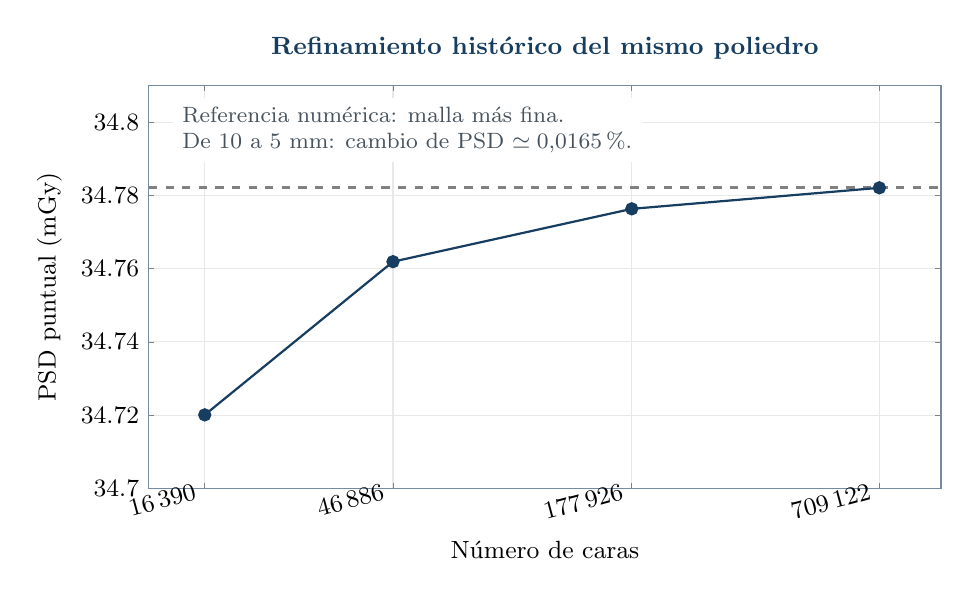
\begin{tikzpicture}
\begin{semilogxaxis}[dermaplot,width=.96\textwidth,height=6.7cm,title={Refinamiento histórico del mismo poliedro},xlabel={Número de caras},ylabel={PSD puntual (mGy)},xmin=12000,xmax=1000000,scaled x ticks=false,xtick={16390,46886,177926,709122},xticklabels={16\,390,46\,886,177\,926,709\,122},x tick label style={rotate=15,anchor=east},ymin=34.70,ymax=34.81,scaled y ticks=false]
\addplot[gray,dashed]coordinates{(12000,34.78205)(1000000,34.78205)};
\addplot[azul,mark=*,thick] coordinates{(16390,34.72008)(46886,34.76189)(177926,34.77631)(709122,34.78205)};
\node[nota,anchor=north west,fill=white]at(rel axis cs:.03,.97){Referencia numérica: malla más fina.\\De 10 a 5 mm: cambio de PSD $\simeq0{,}0165\,\text{\char37}$.};
\end{semilogxaxis}
\end{tikzpicture}

\caption{Estabilidad numérica histórica del máximo al refinar el mismo poliedro. Figura TikZ/PGFPlots reconstruida desde la tabla del antecedente; la malla más fina es referencia numérica, no dosimétrica.}
\end{figure}

\section{Antecedente: rendimiento y límites de comparación}
El estudio previo describe gran ahorro de caché para geometrías idénticas y ahorro pequeño para secuencias de ángulos distintos. Registra además que la preparación, trazado y exportación pueden dominar en momentos diferentes. Sus tiempos se obtuvieron en un entorno Linux virtualizado con control de hilos; no se comparan directamente con una ejecución completa en Windows.

El número de candidatos del índice crecía más deprisa que el número de caras en algunos refinamientos. Esto desaconseja asumir una complejidad global logarítmica por el mero uso de R-tree. Una malla muy fina, un campo oblicuo y una colección grande de eventos pueden producir una carga distinta a la de dos exposiciones de demostración.

La consulta local de métricas sobre vecinos también puede ser costosa: el máximo medio en una región nominal se busca desde caras irradiadas mediante recorridos del grafo. En una ejecución que parece detenida debe distinguirse lectura, preparación, proyección, métricas y escritura. No hay en esta memoria un tiempo medido del caso completo de 101 eventos ni evidencia para diagnosticar un bloqueo concreto del ordenador del usuario.

\section{Pruebas focalizadas repetidas}
La ejecución \codigo{python -m pytest tests/test_azurion.py tests/test_spectral.py tests/test_surface_factors.py -q} termina con 47 pruebas superadas. Se comprueban, entre otras, declaración explícita de filtro no insertado, contradicciones, selección de Al, rechazo de extrapolación, integridad del dataset, promedio de productos y compatibilidad del proveedor.

Las pruebas espectrales incluyen invariancia ante renormalización de fluencia, recuperación de un nodo monoenergético, interpolación del producto entre energías originales, rechazo de entradas inválidas y fracción de kerma exterior. También se prueba la generación de una tabla nueva, su consulta desde el proveedor y la detención ante incompatibilidad con una HVL proporcionada.

En esa prueba de HVL se utiliza un valor calculado para ejercitar la lógica de comparación, y después uno alterado para forzar error. No es una medición física. Superar la prueba demuestra que funciona la condición programada, no que el Azurion cumpla la tolerancia.

\section{Cuatro condiciones clínicas de referencia}
Se repitió la comparación de cuatro casos del informe. La diferencia se define como $\delta_C=100(C_{\mathrm{calc}}/C_{\mathrm{ref}}-1)$. Los espesores son mm y el lado cm.
\begin{table}[htbp]\centering\small
\caption{Comparación parcial del factor combinado con productos clínicos publicados.}
\begin{tabular}{rrrrrrr}\toprule
kVp & Al & Cu & Lado & $C_{\rm ref}$ & $C_{\rm calc}$ & $\delta_C$ (\%)\\\midrule
50 & \num{2.5} & \num{0.0} & 5 & \num{1.211072} & \num{1.209444} & \num{-0.1344}\\
80 & \num{3.1} & \num{0.1} & 20 & \num{1.511424} & \num{1.509847} & \num{-0.1043}\\
100 & \num{4.1} & \num{0.1} & 10 & \num{1.461042} & \num{1.460173} & \num{-0.0595}\\
120 & \num{3.1} & \num{0.3} & 25 & \num{1.662636} & \num{1.660857} & \num{-0.1070}\\
\bottomrule\end{tabular}
\end{table}
Los residuos del combinado se encuentran entre $-\num{0.1344}\,\text{\char37}$ y $-\num{0.0595}\,\text{\char37}$. La comparación también revela diferencias de calidad del haz, presentadas en la tabla siguiente. Un factor combinado parecido no implica que las formas espectrales sean idénticas.
\begin{table}[htbp]\centering\small
\caption{Comparación de HVL1 en las mismas cuatro condiciones.}
\begin{tabular}{rrrrrr}\toprule
kVp & Al & Cu & HVL1 ref. & HVL1 calc. & $\delta_{H_1}$ (\%)\\\midrule
50 & \num{2.5} & \num{0.0} & \num{1.780} & \num{1.734} & \num{-2.597}\\
80 & \num{3.1} & \num{0.1} & \num{4.660} & \num{4.577} & \num{-1.778}\\
100 & \num{4.1} & \num{0.1} & \num{6.170} & \num{6.039} & \num{-2.131}\\
120 & \num{3.1} & \num{0.3} & \num{8.850} & \num{8.679} & \num{-1.934}\\
\bottomrule\end{tabular}
\end{table}
Las diferencias de HVL1 oscilan entre aproximadamente $-\num{2.60}\,\text{\char37}$ y $-\num{1.78}\,\text{\char37}$. No se ajustaron parámetros para anularlas. El informe original usa SpekCalc y sus tablas contienen redondeo y promedios separados; esos elementos forman parte del análisis del residuo.

El contraste no incluye una medida de la instalación. Tampoco demuestra un error inferior al 1\,\% para todo el dominio: cubre cuatro puntos concretos. La tolerancia usada en una prueba automatizada no debe convertirse en una especificación de exactitud del programa.

\section{Convergencia con el paso energético}
Se generaron de nuevo las cuatro condiciones con $\Delta E=1$, \num{0.5}, \num{0.25} y \num{0.125} keV. Se mantuvieron los datos monoenergéticos y el resto de parámetros. La tabla expresa diferencias de $C$ respecto a \num{0.125} keV, en porcentaje; los casos siguen el orden de la comparación clínica.
\begin{table}[htbp]\centering\small
\caption{Sensibilidad del factor combinado al paso energético. Referencia numérica: \num{0.125} keV.}
\begin{tabular}{rrrrr}\toprule
Caso & $\Delta E=1$ & $\Delta E=0{,}5$ & $\Delta E=0{,}25$ & $\Delta E=0{,}125$\\\midrule
1 & \num{0.001856} & \num{0.000361} & \num{0.000085} & \num{0.000000}\\
2 & \num{0.000346} & \num{-0.000258} & \num{0.000116} & \num{0.000000}\\
3 & \num{-0.000740} & \num{-0.000626} & \num{0.000145} & \num{0.000000}\\
4 & \num{-0.001659} & \num{-0.003295} & \num{0.000457} & \num{0.000000}\\
\bottomrule\end{tabular}
\end{table}
Para el paso de trabajo de \num{0.5} keV, la máxima diferencia absoluta en esos cuatro casos es aproximadamente \num{0.00330}\,\%. Es pequeña frente a otras discrepancias del estudio. La variación no es estrictamente monótona, y el refinamiento del generador cambia también la representación de las líneas características.

Este estudio no reduce el intervalo de 5 keV de los factores publicados ni prueba exactitud espectral. Solo examina el discretizado de generación e integración manteniendo el modelo. La tabla fina es una referencia interna, no una medida de verdad física.

\section{Error de consulta entre nodos derivados}
Se seleccionaron nueve puntos interiores que combinan kVp 55, 85 y 115; Cu de \num{0.05}, \num{0.2} y \num{0.3} mm; y lados de \num{7.5}, 15 y 30 cm. Se fijó Al total en \num{4.1} mm. Para cada punto se comparó generar e integrar el espectro directamente con consultar la tabla de 390 filas.
\begin{table}[htbp]\centering\small
\caption{Consulta interpolada frente a integración directa en nueve puntos interiores.}
\begin{tabular}{rrrrrr}\toprule
kVp & Cu & Lado & $C_{\rm directo}$ & $C_{\rm interpolado}$ & $\delta$ (\%)\\\midrule
\num{55} & \num{0.05} & \num{7.5} & \num{1.306526} & \num{1.301831} & \num{-0.3594}\\
\num{55} & \num{0.20} & \num{15.0} & \num{1.433560} & \num{1.420798} & \num{-0.8902}\\
\num{55} & \num{0.30} & \num{30.0} & \num{1.510899} & \num{1.497563} & \num{-0.8827}\\
\num{85} & \num{0.05} & \num{7.5} & \num{1.364223} & \num{1.359837} & \num{-0.3215}\\
\num{85} & \num{0.20} & \num{15.0} & \num{1.528744} & \num{1.516045} & \num{-0.8307}\\
\num{85} & \num{0.30} & \num{30.0} & \num{1.646484} & \num{1.632573} & \num{-0.8449}\\
\num{115} & \num{0.05} & \num{7.5} & \num{1.385523} & \num{1.381972} & \num{-0.2562}\\
\num{115} & \num{0.20} & \num{15.0} & \num{1.551607} & \num{1.541855} & \num{-0.6285}\\
\num{115} & \num{0.30} & \num{30.0} & \num{1.677958} & \num{1.667207} & \num{-0.6407}\\
\bottomrule\end{tabular}
\end{table}
La diferencia va de aproximadamente $-\num{0.8902}\,\text{\char37}$ a $-\num{0.2562}\,\text{\char37}$, con mayor discrepancia que la del paso energético en los cuatro casos anteriores. Este resultado justifica priorizar una evaluación de densidad de nodos y consulta de $C$ antes de reducir indiscriminadamente $\Delta E$.

El ensayo mezcla efectos de interpolación en kVp, Cu y campo, además de la representación por columnas separadas. No permite atribuir todo el residuo a $Bf_{\mathrm{eff}}$ frente a interpolar $C$. Para separar las causas se necesita variar un solo eje y comparar ambos interpoladores con el mismo espectro. La cifra máxima observada tampoco es una cota global del dominio.

\section{Sensibilidad ilustrativa a las hipótesis del tubo}
Se realizó un estudio a 80 kVp, \num{0.1} mm Cu y lado de 20 cm, variando ángulo de ánodo entre 9, 12 y $15^\circ$ y Al fijo entre \num{2.8}, \num{3.1} y \num{3.4} mm. Estas elecciones son escenarios, no intervalos de confianza ni especificaciones acreditadas del Azurion.
\begin{table}[htbp]\centering\small
\caption{Escenarios de ángulo y filtración fija. Diferencia respecto a $12^\circ$ y \num{3.1} mm Al.}
\begin{tabular}{rrrrr}\toprule
Ángulo ($^\circ$) & Al fijo (mm) & $C$ & HVL1 (mm Al) & $\delta_C$ (\%)\\\midrule
\num{9} & \num{2.8} & \num{1.509208} & \num{4.565} & \num{-0.0423}\\
\num{9} & \num{3.1} & \num{1.514819} & \num{4.668} & \num{0.3293}\\
\num{9} & \num{3.4} & \num{1.520143} & \num{4.768} & \num{0.6819}\\
\num{12} & \num{2.8} & \num{1.504017} & \num{4.471} & \num{-0.3861}\\
\num{12} & \num{3.1} & \num{1.509847} & \num{4.577} & \num{0.0000}\\
\num{12} & \num{3.4} & \num{1.515377} & \num{4.679} & \num{0.3663}\\
\num{15} & \num{2.8} & \num{1.500556} & \num{4.410} & \num{-0.6154}\\
\num{15} & \num{3.1} & \num{1.506535} & \num{4.517} & \num{-0.2194}\\
\num{15} & \num{3.4} & \num{1.512203} & \num{4.620} & \num{0.1560}\\
\bottomrule\end{tabular}
\end{table}
En este escenario el factor combinado varía aproximadamente entre $-\num{0.62}\,\text{\char37}$ y $+\num{0.68}\,\text{\char37}$ respecto al caso central, mientras HVL1 también cambia. La similitud de algunos valores de $C$ no elimina la necesidad de caracterización: puede haber degeneración entre parámetros y el resultado absoluto depende además de calibración, mesa y registro.

No se extrapola esta sensibilidad a todos los kVp y filtros. Tampoco se usa para afirmar que la hipótesis de \num{3.1} mm Al sea adecuada. La aportación del estudio es proporcionar una comprobación reproducible y una base para diseñar medidas que discriminen parámetros.

\section{Cobertura del RDSR y ausencia de un resultado clínico final}
El inventario de filtros del capítulo anterior ha sido repetido en esta edición. Bajo Al fijo de \num{3.1} mm, la tabla derivada cubre los kVp y combinaciones Al/Cu de los 101 eventos cuando se consulta a un lado de referencia de 10 cm. Es una comprobación del proveedor, sin malla ni cálculo de campo real.

No se demuestra con ello que los tamaños locales de todos los elementos queden dentro de 5--35 cm, ni que la geometría sea válida. El evento con distancias nulas sigue requiriendo resolución, y la posición del contorno sigue sin registro experimental. No se presenta una PSD del procedimiento como resultado final de esta memoria.

La distinción evita un error de interpretación especialmente relevante: completar un dataset puede resolver un bloqueo informático y, simultáneamente, dejar intactos los principales determinantes de error físico. La utilidad de las nuevas tablas debe evaluarse como parte del sistema completo.
\FloatBarrier

\chapter{Incertidumbre y programa de validación}
\section{Verificación, caracterización y validación}
La verificación responde a si las ecuaciones y políticas elegidas se implementan correctamente. La caracterización aporta parámetros de una instalación. La validación compara predicciones con referencias externas para un uso previsto. Un cálculo puede superar la primera y seguir pendiente de las otras dos.

En DermaDose hay evidencia de lectura controlada, algebra, selección geométrica y consulta tabulada. Hay también hipótesis de equipo y anatomía que condicionan cualquier mapa. La siguiente fase debe producir datos externos capaces de comprobar esos supuestos. El programa escalonado de la figura~\ref{fig:valid} evita comenzar con un procedimiento complejo donde varias causas de discrepancia sean inseparables.
\begin{figure}[htbp]\centering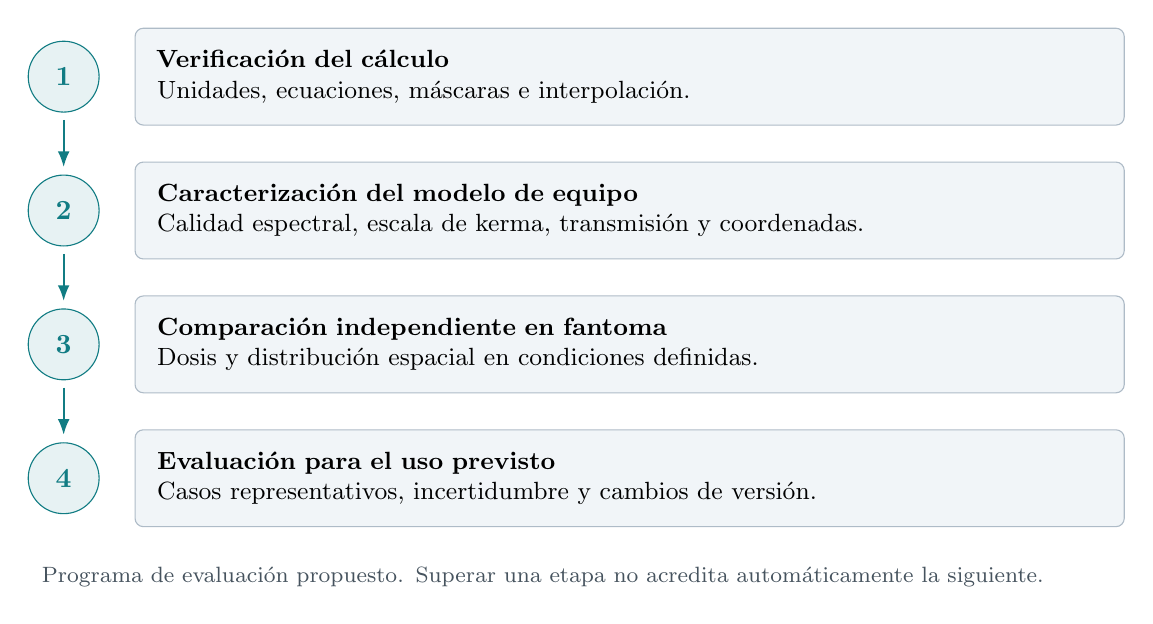
\begin{tikzpicture}[font=\small]
\foreach \y/\n/\titre/\txt in {0/1/{Verificación del cálculo}/{Unidades, ecuaciones, máscaras e interpolación.},-1.7/2/{Caracterización del modelo de equipo}/{Calidad espectral, escala de kerma, transmisión y coordenadas.},-3.4/3/{Comparación independiente en fantoma}/{Dosis y distribución espacial en condiciones definidas.},-5.1/4/{Evaluación para el uso previsto}/{Casos representativos, incertidumbre y cambios de versión.}}{
\node[circle,draw=turquesa,fill=turquesa!10,minimum size=9mm,font=\bfseries,text=turquesa]at(0,\y){\n};
\node[panel,text width=12cm,anchor=west]at(.9,\y){\textbf{\titre}\\\txt};}
\foreach \y in {0,-1.7,-3.4}\draw[flujo,turquesa](0,\y-.55)--(0,\y-1.15);
\node[nota,text width=13cm,anchor=north west]at(-.4,-6.1){Programa de evaluación propuesto. Superar una etapa no acredita automáticamente la siguiente.};
\end{tikzpicture}

\caption{Niveles de evaluación propuestos. Cada nivel necesita evidencia propia y no se obtiene automáticamente del anterior.}\label{fig:valid}\end{figure}

\section{Definir el mensurando antes del ensayo}
Debe especificarse si se compara kerma incidente en aire, kerma superficial de agua o dosis absorbida en una región definida. También se fijarán plano, profundidad, área de promediado, tamaño de campo y presencia de mesa. Una comparación entre una PSD puntual numérica y una lectura integrada por una cámara necesita modelar o acotar esa diferencia de soporte.

Para mapas, hay que definir registro, resolución del detector y regla de muestreo. Una película sobre un cilindro no representa directamente un plano de malla sin transformación. Las coordenadas de dosímetros deben expresarse en el mismo marco que los centroides, con incertidumbre de posición incluida. Un máximo medido entre pocos puntos es el máximo de esos puntos, no necesariamente el de toda la superficie.

El uso previsto determinará qué discrepancias son relevantes. El seguimiento aproximado de regiones irradiadas y una decisión basada en un umbral de dosis exigen evaluaciones distintas. Las tolerancias deben establecerse antes de observar el resultado y justificarse con incertidumbre de referencia y necesidades del uso.

\section{Presupuesto de incertidumbre}
Para un punto donde la máscara no cambia y un producto de factores independientes, una aproximación de primer orden sería
\begin{equation}\label{eq:unc}
u_r^2(D)\simeq u_r^2(\Ka)+4u_r^2(d_r)+4u_r^2(r)+u_r^2(CF)+u_r^2(P)+u_r^2(T)+u_r^2(C),
\end{equation}
con covarianzas adicionales cuando las entradas no sean independientes. La expresión es ilustrativa: $d_r$ y $r$ pueden compartir parámetros geométricos, y la máscara puede cambiar discontinuamente. Aplicarla sin evaluar esas dependencias subestimaría o contaría dos veces componentes.

La incertidumbre del modelo de superficie no se reduce a una escala de dosis. Una traslación puede cambiar el punto del máximo y la superposición de campos. La dispersión de una PSD entre realizaciones mezcla variación del valor y cambio de localización; conviene informar ambos, además de mapas de variabilidad.

En el dataset derivado, $f_{\mathrm{eff}}=C/B$ no es independiente de $B$. Asignar incertidumbres independientes a ambas columnas y combinarlas sin covarianza sería inconsistente. La propagación debería partir de espectro, datos monoenergéticos y parámetros comunes, o trabajar directamente con $C$ y su dependencia documentada.

\begin{table}[htbp]\centering\small
\caption{Componentes que deben evaluarse para el uso de investigación en Azurion.}
\begin{tabularx}{\textwidth}{p{30mm}YY}\toprule
Componente & Obtención propuesta & Situación actual\\\midrule
Indicador $\Ka$ & Cámara trazable, correcciones ambientales y calidad. & No caracterizado en la sala para esta memoria.\\
Calidad espectral & kVp, HVL1, HVL2 y contraste del modelo. & HVL instrumental disponible para ajuste condicionado; caracterización independiente pendiente.\\
Mesa y colchoneta & Cociente transmitido/incidente por calidad y ángulo. & Transmisión sintética de \num{0.8}.\\
Geometría del equipo & Verificación de signos, distancias, campo y mesa. & Perfil de investigación; un evento inválido.\\
Registro anatómico & Puntos de referencia, medidas de distancia y repetibilidad. & Colocación XCAT hipotética.\\
Superficie & Sensibilidad a segmentación, reducción y truncamiento. & Controles geométricos; fidelidad no cuantificada.\\
Interpolación & Consultas interiores frente a generación directa. & Nueve puntos estudiados; sin cota global.\\
Adecuación física & Comparación en fantomas y transporte independiente. & Agua plana aplicada localmente; pendiente.\\\bottomrule
\end{tabularx}
\end{table}

\begin{figure}[htbp]\centering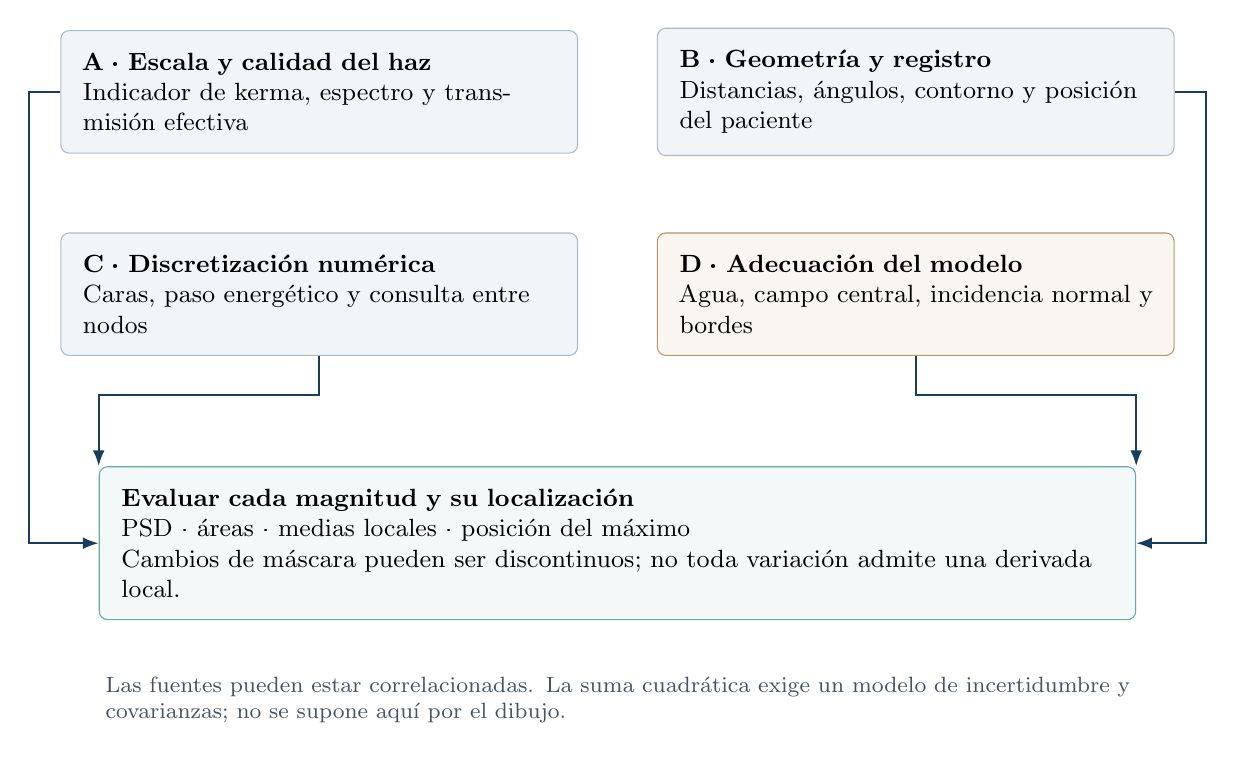
\begin{tikzpicture}[font=\small,node distance=10mm and 10mm]
\node[panel,text width=6cm](a){\textbf{A · Escala y calidad del haz}\\Indicador de kerma, espectro y transmisión efectiva};
\node[panel,text width=6cm,right=of a](b){\textbf{B · Geometría y registro}\\Distancias, ángulos, contorno y posición del paciente};
\node[panel,text width=6cm,below=of a](c){\textbf{C · Discretización numérica}\\Caras, paso energético y consulta entre nodos};
\node[aviso,text width=6cm,right=of c](d){\textbf{D · Adecuación del modelo}\\Agua, campo central, incidencia normal y bordes};
\node[proceso,text width=12.6cm,below=14mm of $(c.south)!.5!(d.south)$](out){\textbf{Evaluar cada magnitud y su localización}\\PSD · áreas · medias locales · posición del máximo\\Cambios de máscara pueden ser discontinuos; no toda variación admite una derivada local.};
\draw[flujo](a.west)--++(-4mm,0)|-(out.west);
\draw[flujo](b.east)--++(4mm,0)|-(out.east);
\draw[flujo](c.south)--++(0,-5mm)-|(out.north west);
\draw[flujo](d.south)--++(0,-5mm)-|(out.north east);
\node[nota,text width=13cm,below=6mm of out]{Las fuentes pueden estar correlacionadas. La suma cuadrática exige un modelo de incertidumbre y covarianzas; no se supone aquí por el dibujo.};
\end{tikzpicture}

\caption{Fuentes de variación y adecuación que condicionan el resultado. Los cuatro bloques no se suponen estadísticamente independientes.}\end{figure}

La incertidumbre numérica observada no debe añadirse automáticamente como si fuese una desviación estándar gaussiana. Una diferencia entre refinamientos es evidencia de sensibilidad, y necesita un modelo de error para incorporarse a un presupuesto probabilístico. Lo mismo ocurre con escenarios hipotéticos de ángulo o Al.

\section{Propagación paramétrica implementada}
El módulo \codigo{uncertainty.py} ofrece muestreo Latin Hypercube o aleatorio, distribuciones normales y uniformes, y lognormales para escalas positivas. En cada realización, un sesgo se comparte entre los eventos. Las dimensiones de entrada se tratan como independientes. El módulo informa una distribución condicionada al modelo y declara que el presupuesto no es completo \citep{jcgm101}.

Ese Monte Carlo es propagación de parámetros, no transporte de fotones. No genera interacciones en el paciente. La independencia asumida puede ser inadecuada si, por ejemplo, una misma calibración afecta varias calidades o si un error de registro correlaciona posiciones.

Las escalas históricas \codigo{bsf_scale} y \codigo{f_skin_scale} buscan factores configurados con esos nombres. No constituyen automáticamente un modelo de incertidumbre del proveedor espectral y pueden carecer de un factor correspondiente en la nueva configuración. La ampliación necesaria es propagar parámetros de generación o una corrección conjunta con correlación definida, y verificar su conexión con el motor.

Cuando una realización queda fuera del dominio, el código interrumpe la propagación en vez de descartarla silenciosamente. Esta política evita condicionar de forma oculta la distribución a los casos que sí se pudieron calcular. La interpretación de cuantiles requiere además estudiar estabilidad frente a tamaño de muestra y semilla.

\section{Caracterización experimental del haz}
\subsection{Inventario previo de la instalación}
Se debe registrar fabricante, modelo exacto, identificador de tubo, ángulo de ánodo documentado, versión de software, limitador, detector, mesa, colchoneta y accesorios. Deben conservarse fecha de medidas y cambios de mantenimiento. La documentación genérica de familia se contrastará con manuales y datos propios de la instalación.

La campaña debe disponer de modos reproducibles que permitan elegir kVp y filtro, evitando que el control automático de exposición cambie simultáneamente variables no registradas. Si se requiere un modo de servicio o coordinación con mantenimiento, se planificará con los responsables de la instalación. El objetivo es caracterizar haces definidos y registrar lo que efectivamente se emitió.

\subsection{HVL y consistencia del generador}
Se propone medir curvas de atenuación en Al en geometría de haz estrecho, minimizando dispersión de los filtros hacia el detector. Se registrarán pureza, espesores, posiciones, tamaño de campo, distancia y estabilidad de salida. La cámara y el electrómetro deben tener calibración y respuesta apropiadas al intervalo de calidad utilizado.

Se medirán al menos las calidades de trabajo sin filtro añadido, con \num{0.1} y \num{0.4} mm Cu más su Al asociado. La cobertura se ampliará si se pretende utilizar \num{0.9} mm Cu. Las tensiones se elegirán para cubrir el intervalo clínico observado, incluyendo extremos y regiones de cambios de modo. La matriz definitiva dependerá de disponibilidad y objetivo, sin inventar ahora un conjunto completo de medidas.

HVL1 y HVL2 permitirán contrastar endurecimiento y homogeneidad. Se evaluará la incertidumbre de interpolación de la curva, variación de salida y efecto de dispersión residual. Los parámetros del espectro se ajustarán sobre un conjunto de caracterización y se comprobarán en calidades reservadas, para evitar presentar un ajuste como validación independiente.

Una filtración equivalente en Al puede ser un parámetro efectivo del modelo. Su acuerdo a una única calidad no prueba que reproduzca todas las componentes de la cadena ni todas las tensiones. Si la identificación es degenerada, se necesitan otras observaciones y restricciones documentales, no más cifras decimales del ajuste.

\subsection{Calibración y rendimiento}
El factor $CF(Q,\mathrm{modo})$ se obtendrá comparando el indicador con una medida de kerma en la referencia adecuada. Se precisará si mesa, colchoneta y retrodispersión están presentes. Se separará el ajuste de calibración de la validación de la distribución superficial.

Cuando se utilice rendimiento por mAs como contraste independiente, se documentarán mAs, pulso, distancia y estabilidad. Releer el mismo $\Ka$ del mismo RDSR no constituye una segunda medida independiente. La normalización absoluta del generador de espectros solo será útil si se caracteriza con ese fin.

\section{Mesa, colchoneta y cambios de calidad}
La campaña debe medir transmisión por kVp, filtro, incidencia y región de paso. Se distinguirá la parte homogénea de raíles o soportes. El cociente transmitido debe definirse con una geometría que limite la dispersión que se desea excluir o incorporar, según el factor modelado.

Se propone contrastar HVL antes y después de la mesa para cuantificar endurecimiento. Si se genera el espectro transmitido y se aplica la ecuación 13 a ese espectro, debe mantenerse coherencia con la transmisión de amplitud del kerma. Si se usa un factor efectivo de dosis que ya incorpora mesa y retrodispersión, el motor no debe multiplicar esas correcciones otra vez.

La separación permite diseñar una evolución del software: mantener un estado espectral para rayos que atraviesan materiales homogéneos o introducir datasets condicionados a trayecto. La elección se justificará por precisión requerida y coste, después de medir la relevancia del efecto.

\section{Verificación geométrica del equipo y del registro}
Se emplearán configuraciones simples con puntos o marcadores de posición conocida. Se comprobarán proyecciones AP, laterales y oblicuas, signos de rotación, orden de ejes, distancia fuente--referencia y plano de campo. Cambiar solo una variable por ensayo ayuda a identificar errores de convención.

Las coordenadas de mesa requieren un origen absoluto o una transformación medida. La referencia al primer evento no proporciona por sí sola posición de anatomía. El registro del contorno puede utilizar landmarks y distancias foco--superficie, con repetición entre operadores para cuantificar variabilidad.

La coherencia de un mapa sobre la cabeza, cuando el procedimiento se dirige a la cabeza, es una comprobación de plausibilidad; no reemplaza una transformación calibrada. Del mismo modo, desplazar visualmente el XCAT hasta que el mapa parezca razonable no demuestra que se haya corregido la geometría.

\section{Ensayos de validación dosimétrica}
Se propone comenzar con una superficie plana o fantoma de agua en incidencia normal y calidad conocida. Después se variarán distancia, campo, ángulo, mesa y superposición. Por último se estudiará un fantoma antropomórfico con región superficial y posicionamiento documentados. Los protocolos aportados ofrecen marcos de ensayo, sin que su mera cita implique conformidad \citep{veridic2020,ganan2024}.

\begin{table}[htbp]\centering\small
\caption{Secuencia propuesta para aislar mecanismos de discrepancia.}
\begin{tabularx}{\textwidth}{p{30mm}YY}\toprule
Ensayo & Variable principal & Resultado que se contrasta\\\midrule
Aire, eje central & Distancia y escala de kerma. & Ley del inverso del cuadrado y $CF$.\\
Fantoma plano & kVp, filtro y campo, sin cambiar registro. & Corrección combinada superficial.\\
Con mesa & Presencia, ángulo y zona de paso. & Transmisión y posible endurecimiento.\\
Contorno curvo & Forma, incidencia y sombras. & Primera entrada, localización y adecuación local de $C$.\\
Varios campos & Desplazamientos y solapamiento. & Mapa acumulado, PSD y áreas.\\
Secuencia realista & Combinación de variables ya caracterizadas. & Comportamiento del sistema para el uso previsto.\\\bottomrule
\end{tabularx}
\end{table}

Para cada ensayo se conservarán RDSR, configuración, geometría, instrumento, calibración, condiciones ambientales y datos brutos. El subconjunto de ajuste no se reutilizará como única validación. Deben repetirse configuraciones para evaluar reproducibilidad y no atribuir a modelo lo que sea reposicionamiento.

\section{Comparación de valores y mapas}
La diferencia relativa $\delta=(D_{\mathrm{calc}}-D_{\mathrm{ref}})/D_{\mathrm{ref}}$ es informativa, pero debe acompañarse de incertidumbre. Una diferencia normalizada coherente emplearía $u_\Delta^2=u_{\mathrm{calc}}^2+u_{\mathrm{ref}}^2-2\operatorname{cov}(D_{\mathrm{calc}},D_{\mathrm{ref}})$, con supuestos documentados. No debe utilizarse una incertidumbre de cálculo cero cuando en realidad no está cuantificada.

La función de comparación escalar disponible divide por la incertidumbre de la medida, no por una incertidumbre combinada completa. El resultado no es automáticamente una prueba estadística de acuerdo. Además, las rutas de validación deben asegurar que preparan el perfil Azurion con las mismas políticas que la ejecución ordinaria; no se ha validado aquí esa integración sobre datos experimentales.

El comparador de mapas existente asocia medidas a centroides próximos mediante KD-tree, limita distancia y evita duplicados. Calcula RMSE, separación entre máximos muestreados y un Dice binario sobre los puntos suministrados. No realiza registro, gamma tridimensional ni Dice de toda una superficie continua. La extensión debe modelar área de lectura y respuesta del detector para comparaciones de mayor rigor.

\section{Referencia de transporte y control de cambios}
Un cálculo Monte Carlo independiente puede contrastar calidad, materiales, espesor, oblicuidad y bordes. Debe reproducir el mismo mensurando: scorer, profundidad, volumen, cortes, normalización y estadística. Una malla de piel con puntuación muy pequeña puede tener un máximo sesgado por ruido, por lo que se estudiará su estabilidad.

La referencia no debe compartir inadvertidamente todas las mismas aproximaciones. Si utiliza el mismo espectro y factores, un acuerdo podría ser circular. Conviene escalonar comparaciones: primero geometría analítica, después transporte en agua y, finalmente, anatomía con materiales. Toda modificación de tabla, parser o malla debe disparar verificaciones de regresión proporcionales a su efecto.
\FloatBarrier

\chapter{Discusión crítica y líneas futuras}
\section{Qué resuelve la ampliación espectral}
La ampliación elimina la necesidad de extrapolar directamente familias clínicas para determinadas combinaciones Al/Cu y permite estudiar 46 kVp mediante una base monoenergética apropiada. También hace más explícita la relación entre calidad del haz y corrección superficial. El cambio más importante es de trazabilidad: se conoce qué espectro calculado y qué datos de respuesta producen cada fila.

El coste de esa flexibilidad es incorporar parámetros del generador que requieren evidencia. El acuerdo con una tabla histórica puede comprobar la implementación, pero no identificar por sí solo el espectro de una sala. Las diferencias pequeñas en $C$ no autorizan a ignorar discrepancias de HVL ni a concluir que la filtración asumida sea correcta.

La vía elegida conserva el transporte en agua del informe original. No añade la dependencia anatómica del paciente. El perfil Azurion debe interpretarse como especialización de lectura y configuración, no como un gemelo físico completo del equipo.

\section{Por qué no se adopta una mezcla automática con factores históricos}
Las constantes históricas cumplen una función de demostración y regresión geométrica. Usarlas selectivamente ante un fallo de dominio produciría un mapa con transiciones de procedencia difíciles de interpretar. Podría incluso generar cambios de dosis que dependiesen de un límite de tabla más que de un cambio físico continuo del haz.

La decisión actual de bloquear en Azurion mantiene el problema visible. Si en el futuro se admite una combinación de fuentes, deberá definirse una jerarquía física, condiciones de uso, continuidad y auditoría por evento, además de validación. No bastaría un mecanismo informático de ``si falla, usar constante''.

El proveedor espectral propio tampoco debe reemplazar siempre una medida válida de la instalación. Cuando existan factores experimentales compatibles y trazables, la elección se basará en calidad de evidencia y mensurando. Mantener intacto el dataset publicado permite comparar vías sin alterar su significado histórico.

\section{Prioridad del registro frente a la apariencia}
La corrección del sombreado responde a un problema de legibilidad: elimina facetas de iluminación. No corrige la colocación anatómica ni una sombra mal calculada. Una representación más continua puede resultar visualmente convincente aunque la región irradiada esté desplazada.

Por tanto, la interpretación del visor debe apoyarse en marcadores geométricos y salidas numéricas, no en plausibilidad visual aislada. La posición del XCAT no se ha modificado en la actualización del visor. La siguiente mejora geométrica debe ser una transformación medida y comprobable, con pruebas de signos y distancias.

Las superficies derivadas de TC ofrecen una oportunidad para reducir discrepancias de forma, pero también introducen una cadena de segmentación y registro. La comodidad de generar un STL no equivale a disponer de una superficie de procedimiento. Será necesario documentar postura, fecha de TC, anatomía truncada y deformación por apoyo.

\section{Prioridades de desarrollo numérico}
El estudio de nueve puntos interiores indica que la interpolación del dataset merece más atención que reducir el paso energético en los cuatro casos examinados. Se propone construir pruebas que separen kVp, Cu y lado, comparando consulta de columnas frente a interpolación directa de $C$. La ampliación de nodos se decidirá con un criterio de error predefinido y puntos de verificación reservados.

Se recomienda extender el benchmark a todas las filas clínicas disponibles y comunicar sesgos por región del dominio. La tabla original incluye redondeo y observaciones documentales que pueden limitar una comparación decimal exacta. Una prueba que únicamente exija diferencias pequeñas en cuatro casos no identifica todos los errores de transcripción o interpolación.

La base monoenergética de paso 5 keV impone otra discretización distinta. Refinar el espectro a \num{0.125} keV no crea nuevos datos de transporte. Si se necesitase resolver estructuras de respuesta no representadas, harían falta datos monoenergéticos adicionales o cálculos independientes, con su propia procedencia.

\section{Prioridades de rendimiento}
La optimización debe seguir una medición por etapas: importación y limpieza, construcción de índice, preselección, primera entrada, factores, métricas, escritura y actualización del visor. Un porcentaje alto de CPU demuestra actividad, pero no identifica el cuello de botella ni permite estimar cuánto falta.

Las mejoras propuestas incluyen progreso por evento, tiempos acumulados por fase, memoria máxima y una salida que distinga cálculo en curso de exportación. El mensaje debe informar trabajo realizado sin prometer un tiempo restante cuando el coste varía con ángulo y candidatos. Un modo que omita métricas locales costosas requiere una opción explícita y una descripción de las salidas omitidas; no se considera implementado por esta memoria.

Para intersecciones se evaluarán BVH o Embree en comparación con la ruta actual, con casos de aristas, autosombra y normales. El uso de GPU se decidirá después de un benchmark equivalente, incluyendo transferencias y tolerancias de precisión. La literatura muestra posibilidades de aceleración, pero no proporciona una ganancia garantizada para este código o su carga \citep{rana2012,takata2018}.

La acumulación por bloques o disco puede reducir la presión de memoria al conservar muchos eventos. También se estudiará una malla gráfica más ligera con correspondencia explícita respecto a la malla de cálculo. No se debe sacrificar la consulta del máximo o mostrar valores suavizados como si pertenecieran a caras realmente calculadas.

\section{Programa de caracterización del Azurion}
Se propone una secuencia con productos revisables, en lugar de marcar de una sola vez un perfil como caracterizado. La tabla siguiente establece dependencias lógicas; no asigna fechas ficticias ni presume disponibilidad de instrumental.
\begin{longtable}{p{12mm}p{33mm}p{57mm}p{36mm}}
\caption{Plan de continuación propuesto y evidencia para avanzar.}\\
\toprule
Fase & Objetivo & Producto verificable & Condición de avance\\\midrule\endfirsthead
\toprule Fase & Objetivo & Producto verificable & Condición de avance\\\midrule\endhead
\bottomrule\endfoot
1 & Identidad de instalación. & Ficha de tubo, versión, limitador, mesa y configuración. & Correspondencia documental y física revisada.\\
2 & Lectura del RDSR. & Corpus anonimizado, matriz de campos y eventos problemáticos. & Unidades y semántica verificadas por caso.\\
3 & Calidad del haz. & Curvas de atenuación, HVL1/HVL2 e incertidumbres. & Modelo contrastado en calidades reservadas.\\
4 & Calibración de kerma. & $CF$ por modo/calidad y trazabilidad instrumental. & Definición libre de doble conteo.\\
5 & Mesa y colchoneta. & Transmisión y contraste de endurecimiento por trayecto. & Representación coherente con $C$.\\
6 & Coordenadas y registro. & Transformación, signos, referencias y repetibilidad. & Errores de localización cuantificados.\\
7 & Factores ampliados. & Dataset versionado, dominio y pruebas de interpolación. & Cobertura del uso previsto sin extrapolación oculta.\\
8 & Validación en fantomas. & Dosis y mapas de referencia independientes. & Criterios previos e incertidumbre compatibles.\\
9 & Evaluación de uso. & Casos representativos y revisión de limitaciones residuales. & Alcance aprobado para una finalidad concreta.\\
\end{longtable}

La caracterización del espectro no debe retrasar indefinidamente otras comprobaciones. Las medidas de geometría y el diagnóstico del evento con distancias nulas pueden avanzar como tareas independientes. La calibración de kerma y la mesa deben conservar definiciones compatibles para integrarse después sin rehacer toda la cadena.

\section{Extensiones físicas justificadas por evidencia}
Una primera extensión es introducir el endurecimiento de mesa en los factores de los rayos que la atraviesan. Otra es estudiar incidencia oblicua y posición respecto al borde, donde la respuesta central de agua puede no representar la distribución local. Los campos alargados justificarían datos de forma o una política de equivalencia contrastada.

Para hueso cercano a superficie, espesores pequeños, salida o dispersión fuera del campo, la aproximación multiplicativa puede resultar insuficiente. En esos casos se evaluará transporte adicional o kernels espaciales, comparando primero situaciones simples. La elección debe responder a una discrepancia observada y a una necesidad del uso, no a añadir complejidad sin posibilidad de validarla.

La reconstrucción temporal de movimientos requiere datos con resolución suficiente. Un RDSR con un único valor por evento no permite inferir cómo cambió continuamente el campo. Si se incorporan logs del equipo o seguimiento del paciente, habrá que validar sincronización, referencias y reparto de kerma antes de acumularlos sobre una superficie.

\section{Trazabilidad de futuras versiones}
Cada perfil de equipo debería declarar identidad, fecha, responsables de revisión, parámetros medidos, incertidumbres, dominio de uso y documento de caracterización. Cada dataset debe tener identificador, versión, archivos y huellas, definición de columnas, generador, parámetros y estado de validación. La procedencia textual no sustituye los registros de medida, pero permite localizarlos.

Los cambios de versión de SpekPy, de tabla o de política de filtración deben tratarse como cambios del modelo, con comparación de resultados. Una actualización que solo modifica iluminación se verifica por otra vía y no exige repetir toda una campaña dosimétrica. Esta proporcionalidad evita tanto omitir pruebas relevantes como repetir trabajos sin relación con el cambio.

\section{Balance científico del estado actual}
El proyecto dispone de una cadena explícita y contrastable para estudiar dosis superficial, y la adaptación Azurion hace visibles datos antes confundidos. La tabla derivada aporta cobertura de calidades bajo hipótesis documentadas. Los nuevos estudios cuantifican comportamiento numérico y delimitan su alcance.

El principal límite sigue siendo la correspondencia entre la representación y la instalación: calidad del haz medida, transmisión, calibración y posición. No se dispone de una incertidumbre clínica completa ni de validación externa propia. La etapa siguiente debe transformar esas ausencias en campañas concretas con referencias independientes, manteniendo el mismo nivel de trazabilidad que ya se exige a las tablas.

\chapter{Fundamento teórico ampliado y atlas conceptual}
\section{Del espectro incidente a la respuesta superficial}
Un espectro no queda determinado por su energía media. Dos distribuciones con igual media pueden producir distinto kerma porque el coeficiente de absorción energética del aire varía con la energía. A su vez, dos distribuciones con igual kerma pueden presentar respuestas superficiales distintas si ponderan de otra manera la función $C(E,s)$. Por ello la integral espectral conserva información que se perdería al sustituir el haz por una única energía.

\begin{figure}[H]\centering
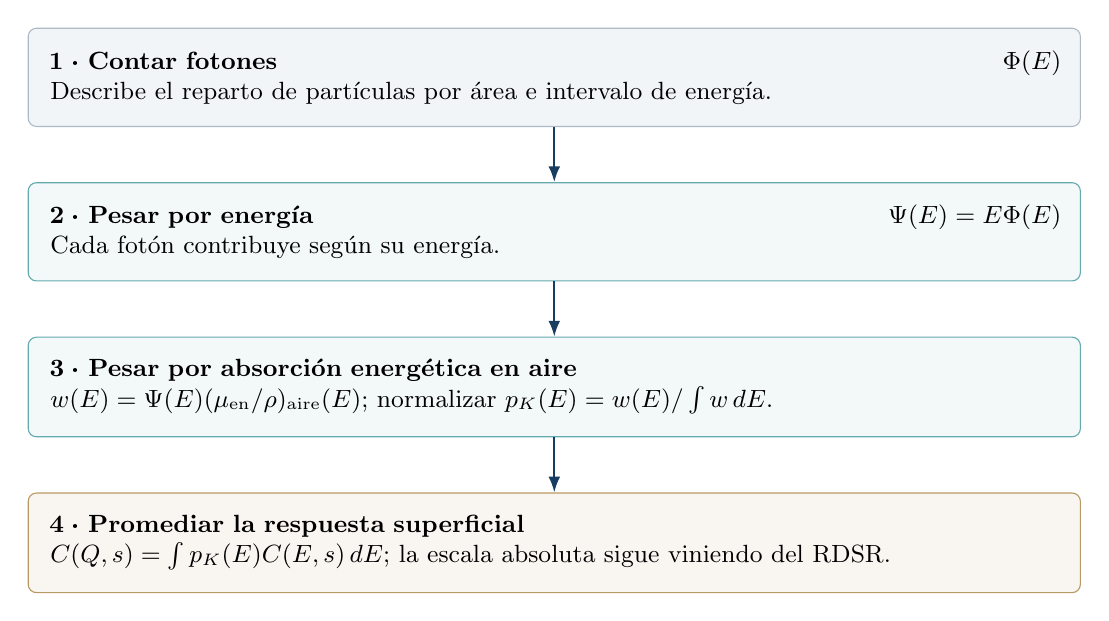
\begin{tikzpicture}[font=\small,node distance=7mm]
\node[panel,text width=12.8cm](a){\textbf{1 · Contar fotones} \hfill $\Phi(E)$\\Describe el reparto de partículas por área e intervalo de energía.};
\node[proceso,text width=12.8cm,below=of a](b){\textbf{2 · Pesar por energía} \hfill $\Psi(E)=E\Phi(E)$\\Cada fotón contribuye según su energía.};
\node[proceso,text width=12.8cm,below=of b](c){\textbf{3 · Pesar por absorción energética en aire}\\$w(E)=\Psi(E)(\mu_{\rm en}/\rho)_{\rm aire}(E)$; normalizar $p_K(E)=w(E)/\int w\,dE$.};
\node[aviso,text width=12.8cm,below=of c](d){\textbf{4 · Promediar la respuesta superficial}\\$C(Q,s)=\int p_K(E)C(E,s)\,dE$; la escala absoluta sigue viniendo del RDSR.};
\foreach \u/\v in {a/b,b/c,c/d}\draw[flujo](\u)--(\v);
\end{tikzpicture}

\caption{Cuatro niveles de ponderación. Cada paso cambia la magnitud descrita; una curva de fotones no es una distribución de kerma.}
\end{figure}
La normalización del espectro desaparece en el cociente, pero su forma permanece. Esta propiedad permite obtener factores relativos desde SpekPy y mantener la escala absoluta del procedimiento en el indicador de kerma y su calibración. No permite deducir una calibración absoluta del equipo a partir del buen comportamiento de un cociente.

\section{Origen de la retrodispersión y aproximación local}
El haz primario deposita energía y genera fotones dispersos con otras direcciones y energías. Parte de esos fotones retorna hacia la entrada. La respuesta superficial depende por ello del volumen irradiado y de los materiales, además de la calidad primaria. El campo de dispersión es espacial: el factor central tabulado condensa una parte de esa información bajo condiciones concretas.
\begin{figure}[H]\centering
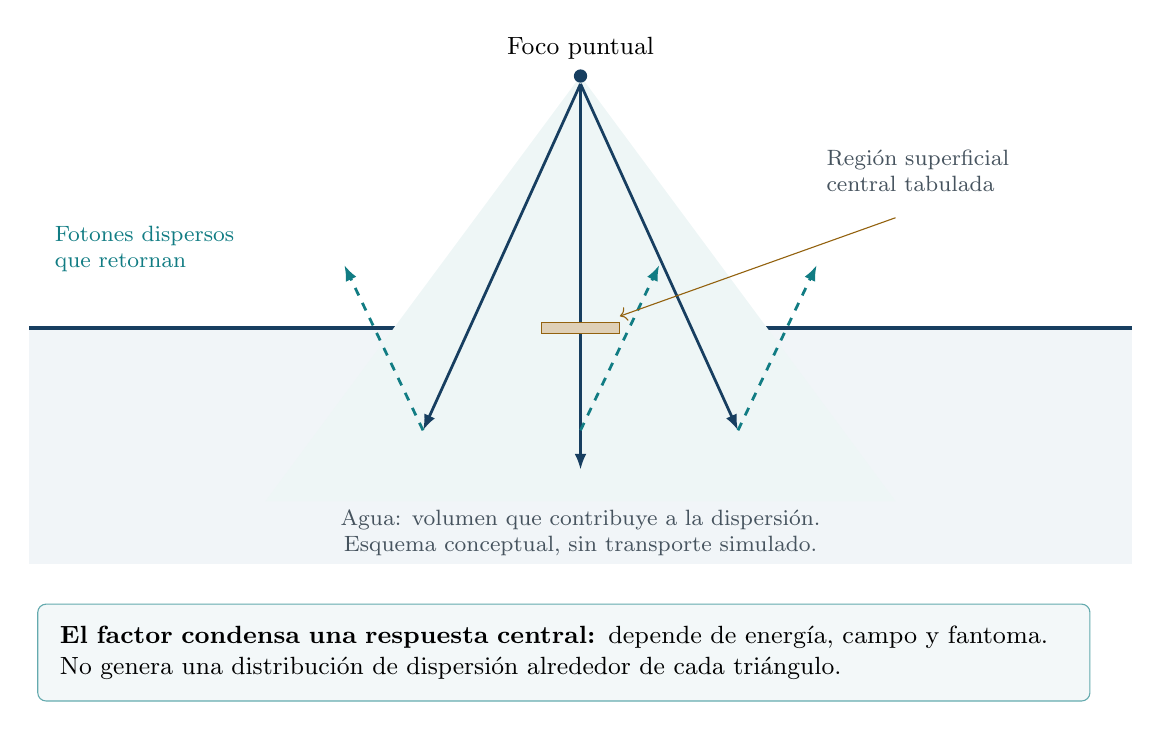
\begin{tikzpicture}[font=\small,x=1cm,y=1cm]
\fill[gris](0,-3)rectangle(14,0);\draw[azul,very thick](0,0)--(14,0);
\fill[turquesa!7](7,3.2)--(3,-2.2)--(11,-2.2)--cycle;
\node[punto,label=above:{Foco puntual}]at(7,3.2){};
\draw[rayo](7,3.1)--(5,-1.3);\draw[rayo](7,3.1)--(9,-1.3);
\draw[rayo](7,3.1)--(7,-1.8);
\foreach \a/\b in {5/4,9/10,7/8}\draw[retorno](\a,-1.3)--(\b,.8);
\draw[ocre,fill=ocre!30](6.5,-.07)rectangle(7.5,.07);
\draw[ocre,->](11,1.4)--(7.5,.15);
\node[nota,anchor=west]at(10,2){Región superficial\\central tabulada};
\node[nota,anchor=west,text=turquesa]at(.2,1){Fotones dispersos\\que retornan};
\node[nota,align=center]at(7,-2.6){Agua: volumen que contribuye a la dispersión.\\Esquema conceptual, sin transporte simulado.};
\node[proceso,text width=12.8cm,anchor=north west]at(.1,-3.5){\textbf{El factor condensa una respuesta central:} depende de energía, campo y fantoma. No genera una distribución de dispersión alrededor de cada triángulo.};
\end{tikzpicture}

\caption{Retrodispersión esquemática. Las flechas ilustran direcciones posibles, sin representar trayectorias simuladas ni probabilidades de interacción.}
\end{figure}
En una superficie curva, aplicar la respuesta de agua plana en cada centroide constituye una aproximación local. Cerca del borde del campo falta parte del volumen que produciría dispersión hacia el punto central de referencia. Aumentar la resolución de la malla no modifica esta limitación: mejora el muestreo de la misma función aproximada.

\section{Kerma y dosis: condiciones de identificación}
El kerma describe transferencia inicial de energía a partículas cargadas; la dosis describe energía impartida en la región considerada. La energía puede cruzar el límite de esa región transportada por electrones secundarios. El equilibrio de partículas cargadas requiere un balance adecuado entre energía que entra y sale, y no debe imponerse automáticamente sobre una interfaz.
\begin{figure}[H]\centering
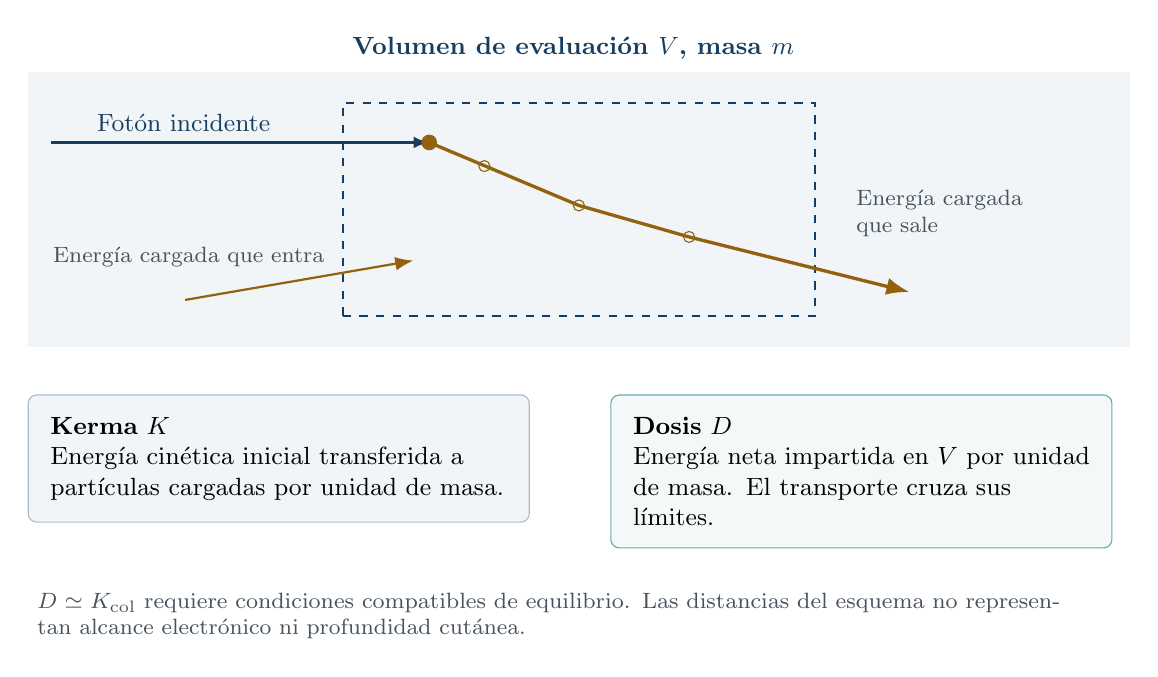
\begin{tikzpicture}[font=\small,x=1cm,y=1cm]
\fill[gris](0,0)rectangle(14,3.5);
\draw[azul,dashed,thick](4,.4)rectangle(10,3.1);
\node[rotulo,anchor=west]at(4,3.8){Volumen de evaluación $V$, masa $m$};
\draw[rayo](.3,2.6)--(5.1,2.6) node[pos=.35,above]{Fotón incidente};
\node[circle,fill=ocre,inner sep=2pt]at(5.1,2.6){};
\draw[-{Latex},ocre,very thick](5.1,2.6)--(7,1.8)--(8.4,1.4)--(11.2,.7);
\node[nota,anchor=west]at(10.4,1.7){Energía cargada\\que sale};
\draw[-{Latex},ocre,thick](2,.6)--(4.9,1.1);
\node[nota,anchor=south west]at(.2,.9){Energía cargada que entra};
\foreach \x/\y in {5.8/2.3,7/1.8,8.4/1.4}\draw[ocre](\x,\y)circle(2pt);
\node[panel,text width=5.8cm,anchor=north west]at(0,-.6){\textbf{Kerma $K$}\\Energía cinética inicial transferida a partículas cargadas por unidad de masa.};
\node[proceso,text width=5.8cm,anchor=north west]at(7.4,-.6){\textbf{Dosis $D$}\\Energía neta impartida en $V$ por unidad de masa. El transporte cruza sus límites.};
\node[nota,text width=13cm,anchor=north west]at(0,-3.0){$D\simeq K_{\rm col}$ requiere condiciones compatibles de equilibrio. Las distancias del esquema no representan alcance electrónico ni profundidad cutánea.};
\end{tikzpicture}

\caption{Distinción conceptual entre transferencia y depósito. El dibujo no establece un alcance electrónico ni una profundidad de piel.}
\end{figure}
La equivalencia aproximada entre dosis y kerma de colisión necesita condiciones físicas y un volumen de evaluación compatibles. La salida superficial de agua del prototipo debe compararse con una referencia que conserve estas definiciones. Cambiar su etiqueta a piel no añade composición tisular ni resuelve transporte electrónico.

\section{La no conmutatividad de los promedios}
Para pesos normalizados, la identidad
\begin{equation}
\langle Bf\rangle_w=\langle B\rangle_w\langle f\rangle_w+
\operatorname{Cov}_w(B,f)
\end{equation}
explica por qué multiplicar promedios no reproduce en general el promedio del producto. La covarianza no representa aquí incertidumbre experimental: es una propiedad algebraica de dos funciones de energía bajo un mismo peso espectral. Si los pesos de los promedios son diferentes, esa identidad ya no basta para relacionarlos.
\begin{figure}[H]\centering
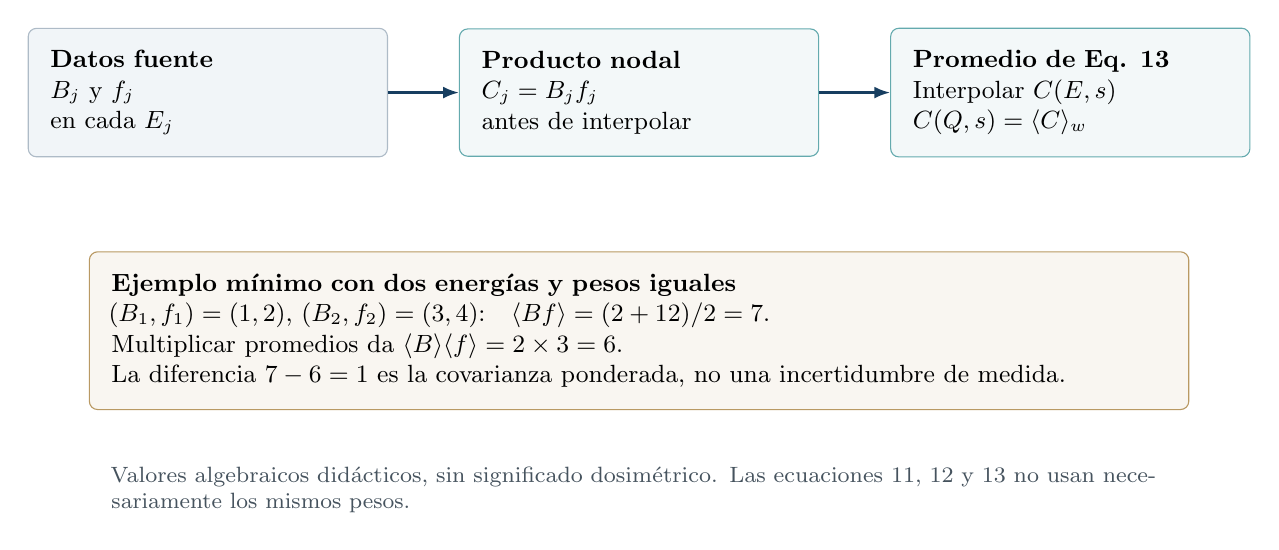
\begin{tikzpicture}[font=\small,node distance=8mm and 9mm]
\node[panel,text width=4cm](a){\textbf{Datos fuente}\\$B_j$ y $f_j$\\en cada $E_j$};
\node[proceso,text width=4cm,right=of a](b){\textbf{Producto nodal}\\$C_j=B_j f_j$\\antes de interpolar};
\node[proceso,text width=4cm,right=of b](c){\textbf{Promedio de Eq. 13}\\Interpolar $C(E,s)$\\$C(Q,s)=\langle C\rangle_w$};
\draw[flujo](a)--(b);\draw[flujo](b)--(c);
\node[aviso,text width=13.4cm,below=12mm of b](ex){\textbf{Ejemplo mínimo con dos energías y pesos iguales}\\$(B_1,f_1)=(1,2)$, $(B_2,f_2)=(3,4)$:\quad $\langle Bf\rangle=(2+12)/2=7$.\\Multiplicar promedios da $\langle B\rangle\langle f\rangle=2\times3=6$.\\La diferencia $7-6=1$ es la covarianza ponderada, no una incertidumbre de medida.};
\node[nota,text width=13.4cm,below=6mm of ex]{Valores algebraicos didácticos, sin significado dosimétrico. Las ecuaciones 11, 12 y 13 no usan necesariamente los mismos pesos.};
\end{tikzpicture}

\caption{Orden de operaciones del cálculo derivado. Alterar el orden de producto, interpolación y promedio define otro procedimiento entre nodos.}
\end{figure}
De manera análoga, interpolar $B$ y $f_{\rm eff}$ por separado no equivale exactamente a interpolar su producto. La discrepancia se estudia numéricamente en esta memoria y motiva la política de interpolación directa de $C$ incorporada en el perfil refinado (capítulo siguiente). Una separación de columnas útil para compatibilidad no debe ocultar la dependencia entre ellas.

\section{Atenuación polienergética y capa hemirreductora}
Para un filtro de espesor $x$ en geometría estrecha, el kerma relativo se representa idealmente mediante
\begin{equation}
R(x)=\frac{\int w(E)e^{-\mu(E)x}dE}{\int w(E)dE}.
\end{equation}
La suma de exponenciales de pendientes distintas no es en general una exponencial única. Al filtrar se eliminan preferentemente componentes de menor energía; cambia la pendiente efectiva de la curva y suele aumentar el espesor adicional necesario para pasar de la mitad al cuarto.
\begin{figure}[H]\centering
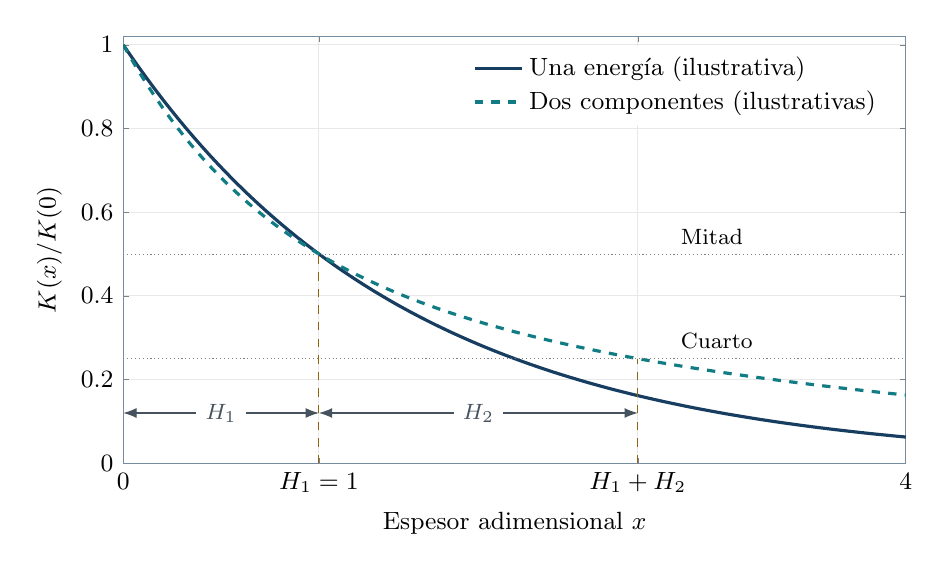
\begin{tikzpicture}
\begin{axis}[dermaplot,height=7cm,xlabel={Espesor adimensional $x$},ylabel={$K(x)/K(0)$},xmin=0,xmax=4,ymin=0,ymax=1.02,legend style={at={(.98,.98)},anchor=north east},xtick={0,1,2.63030,4},xticklabels={0,$H_1=1$,$H_1+H_2$,4}]
\addplot[azul,domain=0:4,samples=101]{exp(-ln(2)*x)};\addlegendentry{Una energía (ilustrativa)}
\addplot[turquesa,dashed,domain=0:4,samples=101]{.5*exp(-1.4*x)+.5*exp(-0.283154953923*x)};\addlegendentry{Dos componentes (ilustrativas)}
\draw[gray,densely dotted](axis cs:0,.5)--(axis cs:4,.5);
\draw[gray,densely dotted](axis cs:0,.25)--(axis cs:4,.25);
\draw[ocre,dashed](axis cs:1,0)--(axis cs:1,.5);
\draw[ocre,dashed](axis cs:2.63030,0)--(axis cs:2.63030,.25);
\draw[cota](axis cs:0,.12)--(axis cs:1,.12)node[midway,fill=white,font=\footnotesize]{$H_1$};
\draw[cota](axis cs:1,.12)--(axis cs:2.63030,.12)node[midway,fill=white,font=\footnotesize]{$H_2$};
\node[font=\footnotesize,anchor=south west]at(axis cs:2.8,.5){Mitad};
\node[font=\footnotesize,anchor=south west]at(axis cs:2.8,.25){Cuarto};
\end{axis}
\end{tikzpicture}

\caption{Atenuación conceptual: dos curvas con la misma primera HVL pueden tener distinta segunda HVL. La segunda es un espesor adicional. Espesores y coeficientes ilustrativos, sin datos del Azurion.}
\end{figure}
La HVL resume esta curva en puntos específicos. Dos curvas pueden cruzar el nivel de la mitad en el mismo espesor y diferir después. Medir también la segunda HVL y otras calidades ayuda a discriminar modelos, pero no garantiza una reconstrucción espectral única. El ajuste debe incorporar restricciones físicas y validación con observaciones reservadas.

\section{Tres errores distintos en una superficie triangular}
La discretización de la forma aproxima el contorno real mediante planos. El muestreo del campo asigna un valor representativo a cada cara. El registro coloca el contorno en el marco del equipo. Estos tres mecanismos pueden producir mapas distintos aun usando exactamente los mismos factores espectrales.
\begin{figure}[H]\centering
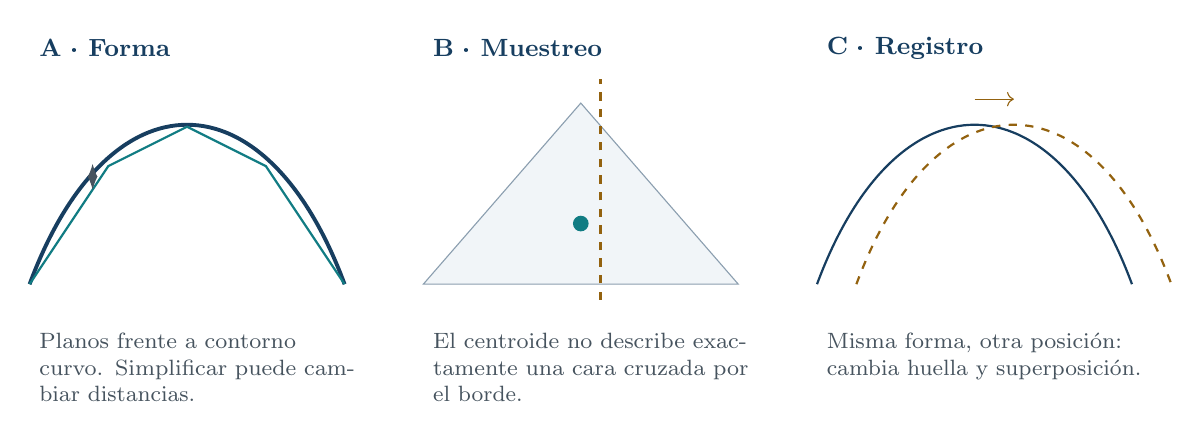
\begin{tikzpicture}[font=\small,x=1cm,y=1cm]
\foreach \x/\titulo in {0/{A · Forma},5/{B · Muestreo},10/{C · Registro}}\node[rotulo,anchor=west]at(\x,3){\titulo};
\draw[azul,line width=1.4pt](0,0)..controls(1,2.7)and(3,2.7)..(4,0);
\draw[turquesa,thick](0,0)--(1,1.5)--(2,2)--(3,1.5)--(4,0);
\draw[cota](.8,1.2)--(.8,1.53);
\node[nota,text width=4cm,anchor=north west]at(0,-.5){Planos frente a contorno curvo. Simplificar puede cambiar distancias.};
\draw[azul!50,fill=gris](5,0)--(9,0)--(7,2.3)--cycle;
\draw[ocre,very thick,dashed](7.25,-.2)--(7.25,2.6);
\node[circle,fill=turquesa,inner sep=2pt]at(7,.77){};
\node[nota,text width=4cm,anchor=north west]at(5,-.5){El centroide no describe exactamente una cara cruzada por el borde.};
\draw[azul,thick](10,0)..controls(11,2.7)and(13,2.7)..(14,0);
\draw[ocre,dashed,thick](10.5,0)..controls(11.5,2.7)and(13.5,2.7)..(14.5,0);
\draw[->,ocre](12,2.35)--(12.5,2.35);
\node[nota,text width=4cm,anchor=north west]at(10,-.5){Misma forma, otra posición: cambia huella y superposición.};
\end{tikzpicture}

\caption{Error de forma y error de muestreo son distintos. Dividir una cara plana mejora el muestreo, pero no recupera la curva anatómica original.}
\end{figure}
La simplificación puede modificar forma y distancias; la subdivisión mantiene el poliedro y cambia el muestreo. Un error de registro desplaza toda la anatomía y altera superposición. Por ello las pruebas de convergencia deben medir máximo, posición y áreas, mientras que el registro requiere referencias geométricas externas.

\section{Síntesis de las dependencias físicas}
El resultado absoluto está condicionado por cuatro relaciones: el indicador con la referencia de kerma; la referencia con la superficie por geometría; el haz con su respuesta superficial; y el contorno representado con la posición real. La caracterización espectral fortalece la tercera relación, pero no sustituye las otras.

La prioridad experimental es medir parámetros que permitan discriminar hipótesis, no solo obtener un mapa visualmente convincente. El acuerdo de HVL controla parte de la calidad; la calibración controla escala; la transmisión controla trayectos; y los marcadores controlan registro. La validación conjunta debe realizarse después de identificar y contrastar esas relaciones por separado.
\FloatBarrier

\chapter{Refinamiento del modelo espectral y de los factores}
\section{Parámetros documentales del tubo}
La documentación de producto de Philips describe un tubo de la familia MRC 200+ GS 0407 con ángulo de ánodo de $11^\circ$ \citep{product0407}. El manual de servicio del MRC 200 0407 confirma directamente este ángulo en Z-1; la hipótesis histórica de $12^\circ$ deja de representar el tubo identificado. El documento corresponde a C20 FlexArm: la correspondencia exacta con la instalación debe confirmarse antes de trasladar otros parámetros geométricos. El cambio se aplica a un perfil de investigación separado.

Los valores de filtración expresados como cobre equivalente no se interpretan automáticamente como espesores físicos de Cu. El modelo conserva por separado aluminio fijo efectivo, aluminio añadido y cobre añadido. No se convierten entre sí mediante una equivalencia constante independiente de energía.

\section{Ajuste del aluminio efectivo mediante calidad del haz}
Se utilizan observaciones instrumentales de primera capa hemirreductora suministradas para estudiar la compatibilidad del espectro. Se dispone de cinco calidades nominales: 50, 60, 80, 100 y 125 kVp, con cuatro observaciones a 80 kVp. No se dispone de una curva de atenuación completa ni de incertidumbres asociadas. Los valores se utilizan como restricciones exploratorias del modelo, sin identificar su información con una caracterización espectral completa.

La filtración añadida de esas observaciones no está especificada. Por ello, el ajuste requiere aceptar explícitamente Cu añadido cero. Se mantiene ánodo W y ángulo de $11^\circ$, y se busca un espesor equivalente de Al entre 1 y 8 mm minimizando
\begin{equation}
J(a)=\frac1N\sum_{q\in\mathcal A}\left[\frac{H_{1,\mathrm{calc}}(V_{q,\mathrm{med}},a)}{H_{1,q,\mathrm{obs}}}-1\right]^2.
\end{equation}
Las observaciones se agrupan por calidad nominal y cada grupo tiene el mismo peso. Así se evita que las repeticiones a 80 kVp dominen el ajuste. Se utiliza tensión medida media por grupo; 50, 60, 80 y 100 kVp participan en el ajuste y 125 kVp se reserva como comprobación interna. No se aplica ponderación por incertidumbre porque sus valores no están establecidos.

El ajuste obtiene $a_{\mathrm{ef}}=\num{4.6137}$ mm Al. El punto reservado de 125 kVp presenta un residuo de HVL1 de \num{1.346}\,\%. Estos residuos no se interpretan como incertidumbre clínica.
\begin{table}[htbp]\centering\small\caption{Ajuste condicionado de HVL1 (mm Al) y cambio del factor combinado a 10 cm de lado.}\resizebox{\textwidth}{!}{\begin{tabular}{rrrrr}\toprule
kVp nominal & HVL1 observada & HVL1 calculada & Residuo (\%) & Cambio $C$ (\%)\\\midrule
\num{50.0000} & \num{2.3200} & \num{2.3978} & \num{3.3517} & \num{2.6432}\\
\num{60.0000} & \num{2.9200} & \num{2.9202} & \num{0.0077} & \num{2.8138}\\
\num{80.0000} & \num{3.9275} & \num{3.8531} & \num{-1.8949} & \num{2.7555}\\
\num{100.0000} & \num{4.8700} & \num{4.7952} & \num{-1.5358} & \num{2.4453}\\
\num{125.0000} & \num{5.8200} & \num{5.8983} & \num{1.3462} & \num{1.9823}\\
\bottomrule\end{tabular}}\end{table}
\begin{figure}[p]\centering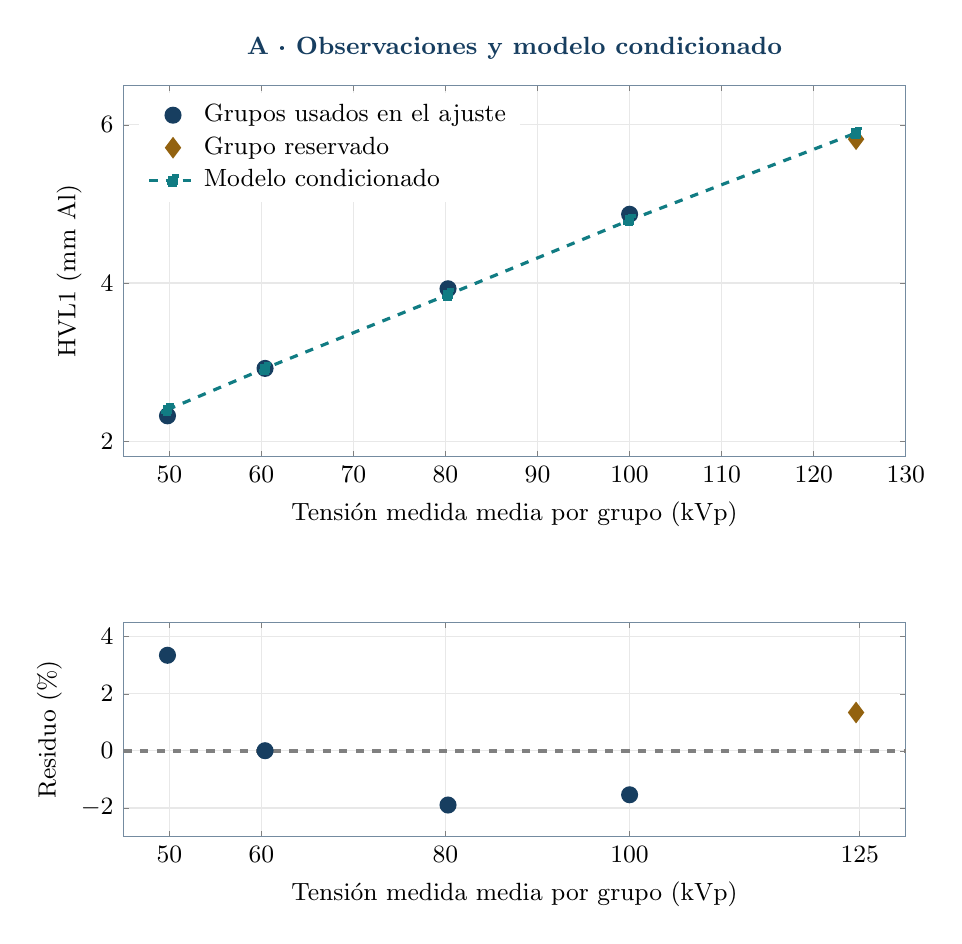
\begin{tikzpicture}
\begin{axis}[dermaplot,name=hvl,height=6.3cm,title={A · Observaciones y modelo condicionado},xlabel={Tensión medida media por grupo (kVp)},ylabel={HVL1 (mm Al)},xmin=45,xmax=130,ymin=1.8,ymax=6.5,legend style={at={(.02,.98)},anchor=north west}]
\addplot[azul,only marks,mark=*,mark size=2.5pt]coordinates{(49.8,2.32)(60.4,2.92)(80.275,3.9275)(100,4.87)};\addlegendentry{Grupos usados en el ajuste}
\addplot[ocre,only marks,mark=diamond*,mark size=3pt]coordinates{(124.6,5.82)};\addlegendentry{Grupo reservado}
\addplot[turquesa,dashed,mark=square*,mark size=1.7pt]coordinates{(49.8,2.39776)(60.4,2.92023)(80.275,3.85308)(100,4.79521)(124.6,5.89835)};\addlegendentry{Modelo condicionado}
\end{axis}
\begin{axis}[dermaplot,at={(hvl.below south west)},anchor=north west,yshift=-1.1cm,height=4.3cm,xlabel={Tensión medida media por grupo (kVp)},ylabel={Residuo (\%)},xmin=45,xmax=130,ymin=-3,ymax=4.5,xtick={50,60,80,100,125}]
\addplot[gray,dashed]coordinates{(45,0)(130,0)};
\addplot[azul,only marks,mark=*,mark size=2.5pt]coordinates{(49.8,3.3517)(60.4,.0077)(80.275,-1.8949)(100,-1.5358)};
\addplot[ocre,only marks,mark=diamond*,mark size=3pt]coordinates{(124.6,1.3462)};
\end{axis}
\end{tikzpicture}

\caption{Compatibilidad del modelo condicionado con HVL1: valores y residuos $100(H_{\rm calc}/H_{\rm obs}-1)$. El grupo de 125 kVp se reserva; los cuatro registros de 80 kVp se agrupan. Sin barras de error porque no se dispone de incertidumbres. Las líneas solo guían la lectura entre calidades.}\label{fig:ajuste_hvl}\end{figure}


El espesor ajustado representa aluminio efectivo dentro del modelo y de la hipótesis de Cu nulo. No identifica por separado filtración inherente, cubierta, colimador y otros componentes. La concordancia de HVL no demuestra unicidad del espectro ni valida la dosis superficial. Es necesario confirmar filtros, tubo y condiciones de las observaciones antes de adoptar el perfil como caracterización de instalación.



\begin{figure}[htbp]\centering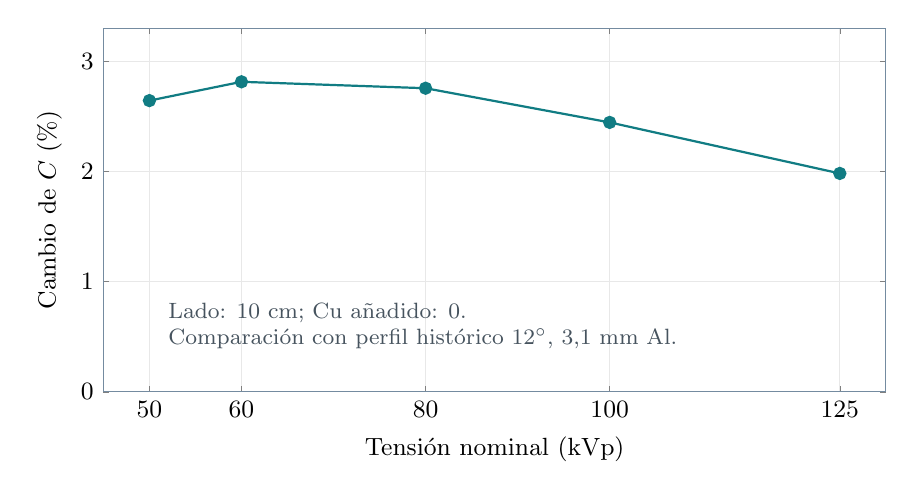
\begin{tikzpicture}
\begin{axis}[dermaplot,height=6.2cm,xlabel={Tensión nominal (kVp)},ylabel={Cambio de $C$ (\%)},xmin=45,xmax=130,ymin=0,ymax=3.3,xtick={50,60,80,100,125}]
\addplot[turquesa,mark=*,thick]coordinates{(50,2.6432)(60,2.8138)(80,2.7555)(100,2.4453)(125,1.9823)};
\node[nota,anchor=south west]at(axis cs:51,.3){Lado: 10 cm; Cu añadido: 0.\\Comparación con perfil histórico $12^\circ$, $3{,}1$ mm Al.};
\end{axis}
\end{tikzpicture}

\caption{Cambio del factor combinado al pasar al perfil condicionado de $11^\circ$ y Al efectivo ajustado. Son diferencias entre modelos, no incertidumbres ni mejoras de exactitud demostradas. Se reutilizan los cinco resultados tabulados de esta memoria.}\label{fig:impacto_factores}\end{figure}

\section{Integración de nuevas calidades}
Se conserva la ecuación 13 del informe de Benmakhlouf y el producto de respuestas monoenergéticas antes del promedio con pesos de kerma. La nueva tabla contiene 13 tensiones, dos familias de Al total (espesor efectivo ajustado y ese espesor más 1 mm Al), siete espesores de Cu (0; 0,1; 0,2; 0,3; 0,4; 0,6; 0,9 mm) y cinco lados de campo (5; 10; 20; 25; 35 cm). Resultan 182 espectros y 910 filas.

Las nuevas filas son calculadas y no constituyen medidas de retrodispersión. En particular, extender el modelo a filtros de cobre no equivale a validarlo con observaciones basales cuya filtración está pendiente de confirmar. Se mantienen el medio de agua, la incidencia normal y las limitaciones de geometría del formalismo original.



\begin{figure}[htbp]\centering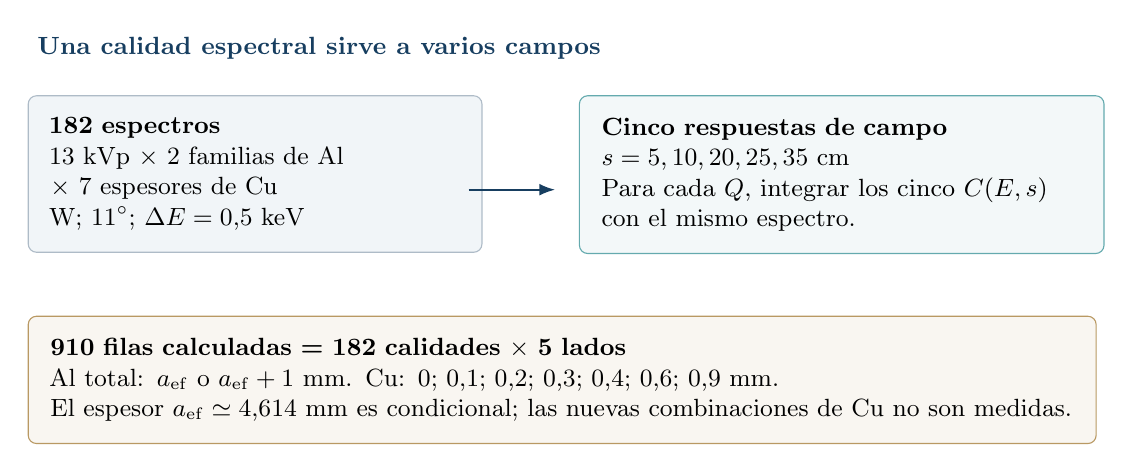
\begin{tikzpicture}[font=\small,x=1cm,y=1cm]
\node[rotulo,anchor=west]at(0,3.5){Una calidad espectral sirve a varios campos};
\node[panel,text width=5.2cm,anchor=north west]at(0,2.9){\textbf{182 espectros}\\13 kVp $\times$ 2 familias de Al\\$\times$ 7 espesores de Cu\\W; $11^\circ$; $\Delta E=0{,}5$ keV};
\node[proceso,text width=6.1cm,anchor=north west]at(7,2.9){\textbf{Cinco respuestas de campo}\\$s=5,10,20,25,35$ cm\\Para cada $Q$, integrar los cinco $C(E,s)$ con el mismo espectro.};
\draw[flujo](5.6,1.7)--(6.7,1.7);
\node[aviso,text width=13cm,anchor=north west]at(0,.1){\textbf{910 filas calculadas = 182 calidades $\times$ 5 lados}\\Al total: $a_{\rm ef}$ o $a_{\rm ef}+1$ mm. Cu: 0; 0,1; 0,2; 0,3; 0,4; 0,6; 0,9 mm.\\El espesor $a_{\rm ef}\simeq4{,}614$ mm es condicional; las nuevas combinaciones de Cu no son medidas.};
\end{tikzpicture}

\caption{Estructura de la tabla calculada ampliada. Se separan el número de espectros y el número de filas, que incluyen el eje de campo. La cobertura de la rejilla no establece validez experimental para cada combinación.}\label{fig:malla_dataset}\end{figure}

\section{Interpolación de la corrección conjunta}
El nuevo dataset interpola directamente $C$, en vez de multiplicar dos interpolantes independientes. Para conservar la interfaz del motor devuelve $B_{\mathrm{interp}}$ y $f_{\mathrm{eff}}=C_{\mathrm{interp}}/B_{\mathrm{interp}}$. Su producto conserva la interpolación elegida para la corrección conjunta.

La política se activa mediante metadatos del nuevo conjunto. Los datos publicados y los datasets anteriores conservan su tratamiento previo. La mejora elimina una aproximación algebraica entre nodos, pero no elimina el error de interpolación de una función física ni habilita extrapolación.

\begin{figure}[htbp]\centering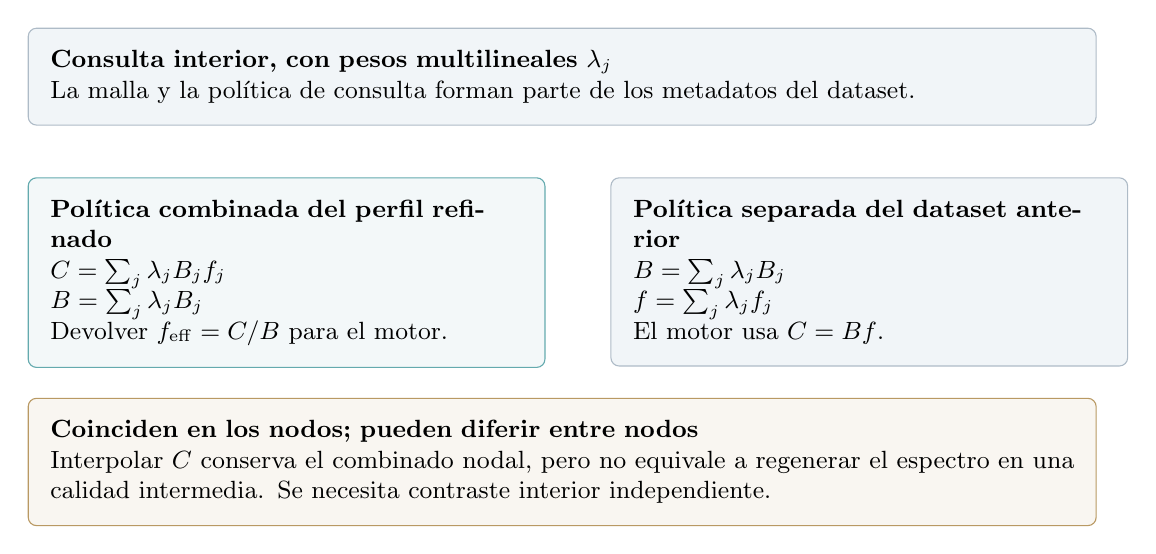
\begin{tikzpicture}[font=\small,x=1cm,y=1cm]
\node[panel,text width=13cm,anchor=north west]at(0,4.6){\textbf{Consulta interior, con pesos multilineales $\lambda_j$}\\La malla y la política de consulta forman parte de los metadatos del dataset.};
\node[proceso,text width=6cm,anchor=north west]at(0,2.7){\textbf{Política combinada del perfil refinado}\\$C=\sum_j\lambda_j B_j f_j$\\$B=\sum_j\lambda_jB_j$\\Devolver $f_{\rm eff}=C/B$ para el motor.};
\node[panel,text width=6cm,anchor=north west]at(7.4,2.7){\textbf{Política separada del dataset anterior}\\$B=\sum_j\lambda_jB_j$\\$f=\sum_j\lambda_jf_j$\\El motor usa $C=Bf$.};
\node[aviso,text width=13cm,anchor=north west]at(0,-.1){\textbf{Coinciden en los nodos; pueden diferir entre nodos}\\Interpolar $C$ conserva el combinado nodal, pero no equivale a regenerar el espectro en una calidad intermedia. Se necesita contraste interior independiente.};
\end{tikzpicture}

\caption{Políticas de interpolación conservadas explícitamente por dataset. La vía combinada opera sobre $C$, manteniendo $f_{\rm eff}=C/B$ por compatibilidad del motor. No sustituye una evaluación del error entre nodos.}\label{fig:consulta_C}\end{figure}

\section{Impacto e interpretación}
En las cinco condiciones basales examinadas y para un lado de 10 cm, el cambio del combinado respecto al modelo anterior es aproximadamente del 2,0 al 2,8 por ciento. No es un cambio predicho de PSD para cualquier procedimiento: el máximo acumulado depende de calidades, campos, registro y superposición.

La extracción de los datos, sus unidades, las hipótesis y las huellas de los archivos fuente permanecen en los registros técnicos de procedencia. Este desarrollo utiliza esas observaciones exclusivamente como información para refinar los factores. No modifica automáticamente la calibración del indicador de kerma, la transmisión de mesa ni la geometría del paciente.

La implementación supera 49 pruebas focalizadas y se han comprobado los 910 nodos de la tabla. No se ha realizado una validación experimental de dosis ni un nuevo mapa clínico completo. El perfil anterior se conserva para comparación y la alternativa ajustada permanece identificada como investigación condicionada.


\FloatBarrier

\chapter{Revisión crítica y correcciones}
\label{chap:auditoria}
\section{Alcance de la evidencia}
La revisión del 29 de octubre de 2026 contrasta la copia disponible del código Python, las rutinas VTK del módulo de Slicer, las tablas y la memoria. Se distinguen errores reproducidos y límites físicos pendientes. No constituye certificación exhaustiva ni validación clínica: faltan recursos originales de fantoma y no se ha ejecutado la interfaz completa dentro de 3D Slicer o en Windows.

La ecuación 13 se contrastó con el informe de Benmakhlouf aportado y la semántica de filtración con DICOM \citep{benreport,dicomfilters}. La disponibilidad de una tabla calculada no demuestra que el espectro real esté caracterizado. El ajuste de un parámetro efectivo a HVL puede no ser identificable si se desconoce la filtración añadida.

\section{Errores confirmados y correcciones}
\begin{enumerate}
\item \textbf{Sustituciones de modelo.} El ejecutable podía reemplazar geometría ante un equipo diferente y sustituir todos los factores por valores sintéticos al salir del dominio publicado. Ahora ambas vías requieren booleanos explícitos independientes, falsos por defecto. Permanecen prohibidas para el perfil Azurion. No se mezclan factores de distinta procedencia por evento.
\item \textbf{Filtración.} La media de espesores mínimo y máximo no determina un espectro transmitido. Se rechazan intervalos no uniformes; se conservan materiales y la distinción entre filtro ausente y dato desconocido. Una etiqueta sintética ya no permite eludir el rechazo de Al añadido.
\item \textbf{Interpolación.} El generador de datasets pasa a versión 1.1 y declara \codigo{interpolation_quantity=combined_C}. Interpola el producto nodal y conserva $f_{\mathrm{eff}}=C/B$. Las tablas históricas no se reescriben; sus políticas permanecen identificadas. El cambio afecta a nuevas tablas y consultas interiores.
\item \textbf{API Python.} Las comprobaciones del perfil Azurion se aplican en el motor, también en llamadas directas. La referencia de mesa de investigación se prepara sobre una copia de configuración, sin mutar la del llamante.
\item \textbf{Máximo promediado.} La búsqueda sobre mallas solo consideraba centros con dosis positiva. Una región de máximo promedio puede estar centrada en una zona nula. Se incluyen todos los centros: dosis $(10,0,10)$ con áreas $(33,34,33)$ mm$^2$ recuperan una media de 6,6 Gy. La vecindad por adyacencia sigue siendo una aproximación discreta. Una elipse sin muestreo longitudinal suficiente ya no devuelve esa métrica.
\item \textbf{Incertidumbre.} Se rechazan incertidumbres RDSR negativas o no finitas y referencias comerciales no finitas. La combinación cuadrática de máximos de componentes declara su hipótesis de covarianza nula: no constituye propagación de incertidumbre de PSD.
\item \textbf{Empaquetado y procedencia.} La distribución instalable incluye los CSV y metadatos del conjunto espectral ampliado. Se elimina la afirmación genérica que identificaba cualquier malla como fantoma de referencia no específico.
\end{enumerate}

\section{Comprobaciones ejecutadas}
La batería disponible produjo \textbf{119 pruebas superadas y 7 fallos}. Los fallos necesitan recursos originales ausentes: \codigo{xcat_wholebody_body.stl}, \codigo{pyskindose_adult_female.stl} y configuraciones asociadas. No se sustituyeron por anatomías inventadas ni se declararon superados. Las pruebas VTK independientes sí se ejecutaron; no verifican toda la interfaz de Slicer.

De 13 casos nuevos, 12 fallan contra la copia anterior y los 13 pasan contra la revisada. Las pruebas antiguas de sustitución se actualizaron para exigir autorización explícita. El caso de filtros homogéneos se separó del caso de intervalo no uniforme.

Se regeneraron 260 espectros: 78 históricos y 182 del conjunto condicionado. Un contraste con interpolación de SciPy de los productos nodales y suma explícita ponderada por kerma reprodujo los 1300 factores combinados almacenados. La máxima diferencia relativa fue menor que $10^{-15}$ y las HVL coincidieron a la precisión numérica disponible. El contraste comparte SpekPy y los datos monoenergéticos: demuestra reproducibilidad algebraica, no independencia física ni una comprobación integral de la transcripción bibliográfica.

Se conservan las tablas originales y sus huellas. La reproducción de cuatro nodos clínicos sigue siendo una comprobación parcial; no acota globalmente el error en todas las geometrías.

\section{Interpretación y límites pendientes}
El factor combinado convierte kerma en aire libre en kerma en agua superficial. Su interpretación como dosis absorbida está condicionada al formalismo y no define dosis a 0,07 mm. El anexo corrige el significado de \codigo{thickness_mm}, que es un argumento de factores y no transporte dentro del paciente. Las inclinaciones y desplazamientos también actúan sobre mallas; el origen local precede a la colocación sobre la mesa. Se explicitan las matrices de rotación sin cambiar signos sin evidencia experimental.

Siguen pendientes la identidad y configuración exactas del tubo, la calidad espectral independiente, transmisión y endurecimiento de mesa, oblicuidad y borde de campo, registro anatómico y comparación dosimétrica externa. Una superficie cerrada puede contener errores anatómicos o autointersecciones no detectadas. El refinamiento no recupera anatomía perdida por segmentación o simplificación. La primera entrada y los factores locales no sustituyen transporte de radiación.

Las correcciones aumentan la trazabilidad y consistencia. No permiten afirmar que todo RDSR de Azurion sea procesable ni que un cálculo terminado esté clínicamente validado.

\chapter{Caracterización documental del MRC 200 0407}
\label{chap:mrc200}
\section{Identidad, fuentes y jerarquía de evidencia}
La identificación del tubo instalado como MRC 200 0407 es aportada por el usuario. El manual de servicio Philips 4512-988-00132, revisión AC, abril de 2011, describe el conjunto ROT-GS1004 y distingue los datos del inserto (Z-1) de los de la carcasa (Z-2) \citep{mrcservice}. Las instrucciones oficiales Azurion Release 2.2 ofrecen ejemplos de etiquetas compatibles y especificaciones del limitador \citep{azurion22}. No se equipara automáticamente esta variante con MRC 200+; no se transfieren características térmicas del modelo con signo más.

\begin{table}[htbp]\centering\small
\begin{tabularx}{\linewidth}{l l X}\toprule
Magnitud & Valor documental & Aplicación en DermaDose\\\midrule
Ángulo anódico & $11^\circ$ & Generación del espectro central\\
Focos nominales & 0,4 / 0,7 mm & Metadatos; no modelo de penumbra\\
Límite del conjunto & 125 kV & Rechazo explícito de eventos superiores\\
Filtración inherente & 0,8 mm Al eq. & Componente ya incluido en el total\\
Placa del conjunto & 1,7 mm Al & Incluida en el mínimo del conjunto\\
Mínimo del conjunto & 2,5 mm Al eq. & Escenario nominal, no medida efectiva\\
Disco anódico & 200 mm & Identificación, sin multiplicador de dosis\\\bottomrule
\end{tabularx}\caption{Datos documentales del MRC 200 0407 y uso efectivo. El material del ánodo se describe como compuesto de tungsteno aleado con renio RT/TZM; SpekPy utiliza aquí una aproximación de blanco W.}\end{table}
El inserto tiene una tensión nominal de 150 kV con nota de reducción por la carcasa. El límite aplicable al conjunto es 125 kV. Ni el diámetro del disco ni las capacidades térmicas son factores multiplicativos de dosis. No se reconstruye la emisión térmica ni se deduce el rendimiento del tubo a partir de sus potencias nominales.

\section{Filtración: componentes y equivalencia}
El mínimo de 2,5 mm Al equivalente incluye la contribución inherente de 0,8 mm Al equivalente y la placa de 1,7 mm Al. Sumarlos nuevamente al total duplicaría la filtración. La equivalencia en aluminio se define bajo una calidad de referencia; no implica identidad de espectros con una placa homogénea de Al a cualquier tensión. Por ello, emplear 2,5 mm de Al en SpekPy constituye un escenario nominal documentado, no la caracterización completa de la instalación.

\begin{figure}[htbp]\centering
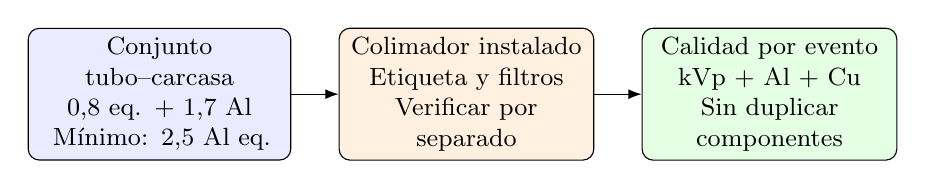
\begin{tikzpicture}[font=\small,>=Latex]
\node[draw,rounded corners,fill=blue!8,text width=3.1cm,align=center] (a) {Conjunto tubo--carcasa\\0,8 eq. + 1,7 Al\\Mínimo: 2,5 Al eq.};
\node[draw,rounded corners,fill=orange!12,text width=3cm,align=center,right=6mm of a] (b) {Colimador instalado\\Etiqueta y filtros\\Verificar por separado};
\node[draw,rounded corners,fill=green!10,text width=3cm,align=center,right=6mm of b] (c) {Calidad por evento\\kVp + Al + Cu\\Sin duplicar componentes};
\draw[->] (a)--(b);\draw[->] (b)--(c);
\end{tikzpicture}\caption{Contabilidad física de filtración. Las equivalencias nominales no sustituyen una caracterización espectral y geométrica del equipo instalado.}\end{figure}
Las etiquetas de ejemplo del limitador en el IFU declaran 0,1 mm Al equivalente. Se calculan dos escenarios: conjunto nominal (2,5 mm) y conjunto más esa contribución nominal (2,6 mm). La suma de equivalencias se utiliza únicamente como aproximación de modelado. Deben verificarse el limitador instalado y los componentes ya incluidos en cualquier ajuste experimental. El IFU, página 403, documenta filtros 0,1/0,4/0,9 mm Cu acompañados por 1 mm Al para la familia de limitadores indicada. Las equivalencias de esos filtros no se añaden además de sus espesores materiales. No se inventa aluminio acompañante cuando el evento no lo declara: su ausencia exige investigar el mapeo de la instalación.

\section{Tablas calculadas y trazabilidad}
El nuevo dataset separado emplea SpekPy 2.5.4, W, ángulo de $11^\circ$ y paso energético 0,5 keV. Se incluyen tensiones 46, 50, 60, 70, 80, 90, 100, 110, 120 y 125 kV; Al de 2,5, 2,6, 3,5 y 3,6 mm; Cu de 0, 0,1, 0,2, 0,3, 0,4, 0,6 y 0,9 mm; campos cuadrados de lado 5, 10, 20, 25 y 35 cm. Los nodos adicionales de Cu son coordenadas del modelo, no posiciones nuevas atribuidas al equipo. Las familias con 1 mm Al adicional permiten representar eventos que efectivamente lo declaren. Se mantienen las tablas originales y el ajuste condicionado previo como modelos distintos, sin sobrescribirlos.
\begin{equation}
C(Q,s)=\frac{\int \Phi(E)\,E\,(\mu_{\mathrm{en}}/\rho)_{\mathrm{aire}}(E)\,B(E,s)\,f(E,s)\,\mathrm dE}{\int \Phi(E)\,E\,(\mu_{\mathrm{en}}/\rho)_{\mathrm{aire}}(E)\,\mathrm dE}.
\end{equation}
La integración sigue los datos monoenergéticos y el formalismo ya descritos. Se conserva el control de energía excluida y la interpolación del factor combinado $C$; el factor de conversión almacenado es $C/B$, no una media independiente de cocientes. El dataset registra versiones, hashes, HVL calculadas y ausencia de validación clínica. El esquema histórico llama \texttt{inherent\_al\_mm} a la coordenada Al: en estos perfiles significa Al fijo efectivo del modelo y no exclusivamente filtración inherente física.

\section{Geometría, límites e interpretación}
El conocimiento del ángulo del ánodo no modifica el ángulo del arco ni establece el eje ánodo--cátodo en coordenadas del paciente. No permite introducir un efecto talón espacial sin orientación y comprobación del perfil. Tampoco determina SID, distancia foco--piel, calibración del kerma, transmisión de mesa, posición del paciente o registro TC--procedimiento. Los nuevos ejemplos rechazan distancias inválidas y no referencian automáticamente la mesa al primer evento. La configuración heredada del XCAT sigue siendo una hipótesis de colocación que debe revisarse.

Los perfiles nuevos comprueban identidad, coherencia de Al entre caracterización y proveedor, ángulo de las tablas y tensión máxima del conjunto. Los datos fuera del dominio siguen produciendo error; no se recortan ni se sustituyen por factores históricos. No se infiere filtro cero a partir de un dato ausente. El conjunto de pruebas verifica estas propiedades además de las regresiones físicas previas. No constituye una validación independiente de exactitud clínica.

La nueva información mejora la especificidad documental y elimina hipótesis incorrectas sobre identidad y ángulo. No demuestra por sí sola menor error dosimétrico. Una HVL única no identifica unívocamente el espectro; la verificación de calidad del haz, filtración seleccionada, orientación y respuesta dosimétrica seguirá siendo necesaria para reducir la incertidumbre. En particular, sustituir un Al efectivo ajustado por un mínimo de catálogo puede empeorar la representación del haz.

\section{Comparación numérica y verificación de la entrega}
En una matriz de 64 casos (50, 80, 100 y 125 kV; Cu de 0, 0,1, 0,4 y 0,9 mm; lados de 5, 10, 20 y 35 cm), se comparó el factor combinado con el modelo histórico de $12^\circ$ y 3,1 mm Al. Para Cu positivo se declara en esta comparación 1 mm Al acompañante en todos los modelos. Cambiar solamente el ángulo a $11^\circ$ produjo diferencias entre $-0,0132\,\text{\char37}$ y $+0,2193\,\text{\char37}$. El escenario nominal de conjunto de 2,5 mm a $11^\circ$ produjo diferencias entre $-1,7083\,\text{\char37}$ y $+0,0012\,\text{\char37}$; con 2,6 mm, entre $-1,3694\,\text{\char37}$ y $-0,0005\,\text{\char37}$. Estas diferencias afectan a $C$ a igualdad de las demás condiciones; no equivalen a una evaluación completa del mapa de un paciente ni a una incertidumbre.

La entrega supera 136 pruebas del programa, incluidas ocho comprobaciones nuevas de identidad de componentes, límites de tensión, coherencia de filtración, carga del dataset y ángulo anódico. Se conserva el caso sintético reproducible anterior para comprobar que la ampliación no altera su resultado. Los valores esperados de ese caso son regresiones del motor y no medidas dosimétricas independientes.

\chapter{Conclusiones}
DermaDose implementa una reconstrucción de irradiación de entrada sobre superficies mediante eventos RDSR, geometría divergente, primera intersección y factores multiplicativos. El modelo permite acumular mapas y estudiar máximos y áreas con procedencia identificada. Su capacidad actual es de investigación y verificación; no se ha establecido exactitud clínica para una instalación.

La adaptación a Philips Azurion ha corregido la interpretación de filtros explícitamente no insertados, mantiene separados aluminio y cobre y selecciona de forma trazable filtración fija más añadida. La lectura del RDSR de trabajo recupera 101 eventos. Permanece un evento con distancias inválidas y falta una transformación anatómica caracterizada, de modo que la lectura satisfactoria no equivale a un mapa físicamente validado.

La ampliación espectral aplica la ecuación 13 del informe de Benmakhlouf a espectros calculados con SpekPy 2.5.4. Utiliza el producto de los factores en sus nodos monoenergéticos y pesos de kerma en aire, sin sustituir el espectro por una energía media. El primer dataset histórico derivado contiene 390 filas para 78 calidades y cinco campos. Es una producción propia, diferenciada de las tablas clínicas publicadas.

La descomposición almacenada mediante $f_{\mathrm{eff}}=C/B$ conserva el combinado en los nodos, pero no reproduce la ecuación 12 como promedio independiente. Su consulta entre nodos introduce una aproximación adicional, cuantificada de forma exploratoria en esta edición. Esta distinción debe mantenerse tanto en el código como en las explicaciones del proyecto.

En la fase histórica descrita se superaron 47 pruebas focalizadas. En cuatro condiciones clínicas de referencia, el factor combinado calculado difiere aproximadamente entre $-\num{0.14}\,\text{\char37}$ y $-\num{0.06}\,\text{\char37}$, mientras HVL1 presenta residuos de aproximadamente $-\num{2.60}\,\text{\char37}$ a $-\num{1.78}\,\text{\char37}$. Nueve consultas interiores muestran diferencias de hasta \num{0.89}\,\% respecto a integración directa. Son resultados numéricos acotados, sin equivalencia con incertidumbre clínica ni cota global de error.

La extracción en Slicer y la reducción con objetivo de \num{150000} triángulos mejoran la preparación de superficies, subordinando la simplificación a su validez. El ajuste visual del visor elimina iluminación por facetas sin cambiar dosis o posición del XCAT. Ninguna de estas mejoras resuelve por sí sola el registro anatómico ni añade física en profundidad.

La continuidad científicamente justificada consiste en caracterizar el tubo y haz de la instalación, medir calibración y transmisión, verificar geometría y registro, y validar con fantomas y referencias independientes. Hasta completar esa evidencia, los parámetros de \num{3.1} mm Al y $12^\circ$ se mantienen como hipótesis y el resultado debe interpretarse como estimación condicionada al modelo de investigación.

La actualización del 26 de octubre incorpora observaciones instrumentales de calidad del haz y la documentación de la familia de tubo 0407. Bajo Cu añadido nulo no confirmado, el ajuste de aluminio efectivo a cuatro calidades da aproximadamente 4,614 mm Al; el punto reservado de 125 kVp presenta un residuo de HVL1 del 1,35 por ciento. Se amplía el dominio calculado a 0,9 mm Cu y se introduce interpolación directa de la corrección conjunta en un nuevo dataset de 910 filas. Las 49 pruebas focalizadas superadas comprueban implementación y regresión; la identidad exacta del tubo, la filtración asociada a las observaciones y la validación de dosis siguen pendientes. No se activa automáticamente una calibración de kerma ni una transmisión de mesa derivadas de datos ambiguos.

La actualización del MRC 200 0407 incorpora tablas nuevas de 1400 filas a $11^\circ$ y escenarios nominales explícitos de filtración, sin declarar una mejora de exactitud clínica. El mínimo de 2,5 mm Al equivalente corresponde al conjunto e incluye sus componentes; no sustituye un Al efectivo medido o ajustado. Los límites del conjunto y la coherencia entre perfil y tablas se verifican automáticamente. Los resultados de comparación y pruebas de esta entrega se conservan con el código.

\clearpage\addcontentsline{toc}{chapter}{Bibliografía}
\bibliographystyle{unsrtnat}
\bibliography{bibliografia}
\appendix
\chapter{Símbolos, unidades y definiciones operativas}
\begin{longtable}{p{27mm}p{80mm}p{29mm}}
\caption{Notación principal de la memoria.}\\
\toprule Símbolo & Definición & Unidad\\\midrule\endfirsthead
\toprule Símbolo & Definición & Unidad\\\midrule\endhead
\bottomrule\endfoot
$e$ & Evento de irradiación. & Índice.\\
$i$ & Elemento superficial o bin, según contexto explícito. & Índice.\\
$\vect p_i$ & Centroide o punto representativo del elemento. & mm.\\
$A_i$ & Área del elemento superficial. & mm$^2$.\\
$\vect s_e$ & Posición del foco. & mm.\\
$\vect b_e$ & Dirección unitaria del eje del haz. & Adimensional.\\
$\vect u_e,\vect v_e$ & Direcciones transversales del haz. & Adimensional.\\
$r_e$ & Distancia euclídea foco--punto. & mm.\\
$t_e$ & Profundidad axial respecto al foco. & mm.\\
$d_{r,e}$ & Distancia foco--referencia del indicador de kerma. & mm.\\
$d_{f,e}$ & Distancia del plano donde se declaran dimensiones de campo. & mm.\\
$w_e,h_e$ & Dimensiones de campo en su plano declarado. & mm.\\
$A_\perp$ & Área de sección del haz normal al eje a profundidad local. & cm$^2$.\\
$s$ & Lado de campo cuadrado o de igual área. & cm.\\
$\Ka$ & Kerma en aire en el punto de referencia intervencionista. & Gy.\\
$P_{KA}$ & Producto kerma-área. & Gy m$^2$ interno.\\
$M_e$ & Máscara de primera entrada. & 0 o 1.\\
$CF$ & Corrección de calibración del indicador. & Adimensional.\\
$P$ & Perfil relativo normalizado del haz. & Adimensional.\\
$T$ & Transmisión aplicada si se cruza mesa. & Adimensional.\\
$B$ & Factor de retrodispersión evaluado en aire. & Adimensional.\\
$f$ & Conversión superficial agua--aire de la fuente. & Adimensional.\\
$C$ & Corrección conjunta superficial, $Bf$. & Adimensional.\\
$f_{\mathrm{eff}}$ & Cociente derivado $C/B$ para interfaz del motor. & Adimensional.\\
$Q$ & Calidad del haz, con parámetros y modelo declarados. & Descriptor.\\
$\Phi(E)$ & Fluencia diferencial de fotones. & Área$^{-1}$ energía$^{-1}$.\\
$\mu/\rho$ & Coeficiente másico de atenuación total. & cm$^2$/g.\\
$\mu_{\mathrm{en}}/\rho$ & Coeficiente másico de absorción de energía. & cm$^2$/g.\\
$w_i$ & Peso de kerma espectral no normalizado. & Proporcional a kerma.\\
$H_1,H_2$ & Primera y segunda capa hemirreductora adicional. & mm Al.\\
$h$ & Coeficiente de homogeneidad $H_1/H_2$. & Adimensional.\\
PSD & Máximo de dosis acumulada según soporte declarado. & Gy.\\
\end{longtable}
\section{Conversiones que requieren control}
Se mantienen $1$ cm $=10$ mm, $1$ cm$^2=100$ mm$^2$, $1$ Gy $=1000$ mGy y $1$ Gy cm$^2=10^{-4}$ Gy m$^2$. La multiplicación por energía en keV es coherente para pesos relativos si toda la integral utiliza esa escala. Para obtener kerma absoluto desde fluencia sería necesaria la conversión a joule y la convención de masa; esa operación no se utiliza para normalizar el mapa desde SpekPy.

El símbolo kVp expresa tensión de pico, no una energía media de los fotones. Una HVL no es un espesor de Al físicamente presente en el equipo y un espesor equivalente de atenuación a una calidad no es una sustitución universal de un material por otro.

\chapter{Configuración y ejecución reproducible}
\section{Organización de carpetas}
La configuración espectral del desarrollo está en \codigo{config/equipo_philips_azurion_espectral_investigacion.json}. Desde esa carpeta, sus rutas relativas apuntan a \codigo{../skindose_verifier/data/derived_azurion_spekpy} y al STL bajo \codigo{../skindose_verifier/data/}. El dataset contiene CSV y metadatos, mientras el informe de paciente permanece fuera de esos recursos.

Si el JSON se copia a \codigo{ejemplos rdsr/ejemplo07}, deben ajustarse las rutas respecto a esa ubicación. Con el paquete en una carpeta hermana denominada \codigo{DermaDose}, la ruta del dataset pasa a ser \codigo{../../DermaDose/skindose_verifier/data/derived_azurion_spekpy}. El nombre exacto debe verificarse en la instalación.

El lanzador histórico puede seleccionar el primer JSON de la carpeta. No se debe colocar \codigo{metadata.json} del dataset como si fuera un perfil de equipo, ni confiar en un orden accidental entre configuraciones. Una ejecución explícita con \codigo{--config} hace inequívoca la elección.

\section{Fragmento del proveedor superficial}
El bloque siguiente es parte de un JSON completo. No puede ejecutarse como perfil autónomo: faltan versión, geometría, paciente y factores de equipo.
\begin{lstlisting}
"surface_factors": {
  "provider": "tabulated_water",
  "dataset_directory": "../skindose_verifier/data/derived_azurion_spekpy",
  "inherent_al_mm": 3.1,
  "target": "W",
  "aluminium_policy": "fixed_plus_event",
  "field_shape_policy": "equal_area",
  "out_of_domain": "error",
  "incident_kerma_basis": "free_in_air_without_backscatter",
  "quality_basis": "event_kvp_filtration_proxy_at_surface",
  "provenance": "Research spectrum assumptions; not measured HVL",
  "allow_water_phantom_approximation": true
}
\end{lstlisting}
La clave Al describe aquí la hipótesis fija. No se cambia a 4,1 mm para eventos que ya declaran 1 mm añadido, porque la política lo sumaría de nuevo. El perfil de equipo y el dataset deben mantenerse coherentes.

\section{Inspección sin malla y cálculo}
Desde la raíz del paquete, esta llamada permite estudiar recuentos y filtración sin calcular dosis:
\begin{lstlisting}
python -m skindose_verifier.azurion RUTA_RDSR.dcm --fixed-al-mm 3.1
\end{lstlisting}
El argumento de Al es una hipótesis explícita de inspección y no modifica el DICOM. El resultado no indica que el procedimiento esté físicamente validado.

Consultar las filas distribuidas no requiere SpekPy; regenerarlas sí. El cálculo normal requiere dependencias del paquete, STL accesible y transformaciones válidas:
\begin{lstlisting}
python -m skindose_verifier run RUTA_RDSR.dcm \
  --config config/equipo_philips_azurion_espectral_investigacion.json \
  --out resultados_espectrales --stage skin_dose
\end{lstlisting}
La barra de continuación pertenece a una terminal tipo Unix. En PowerShell puede escribirse todo en una línea y utilizar \codigo{.venv\Scripts\python.exe}. El comando no garantiza éxito si persisten geometría inválida o consultas fuera de dominio.

\section{Regeneración con procedencia propia}
Una regeneración debe elegir una carpeta nueva. Los parámetros siguientes reproducen las hipótesis de investigación, no una caracterización:
\begin{lstlisting}
python -m pip install -r requirements-spectral.txt
python -m skindose_verifier.spectral benchmark \
  --anode-angle 12 --out comparacion_nueva.json
python -m skindose_verifier.spectral build \
  --out tablas_espectrales_nuevas \
  --kvps 46,50,60,70,80,90,100,110,120,125,130,140,150 \
  --al 3.1,4.1 --cu 0,0.1,0.4 --fields 5,10,20,25,35 \
  --anode-angle 12
\end{lstlisting}
La dependencia se fija en \codigo{spekpy==2.5.4}. Al utilizar datos medidos se revisarán parámetros y versiones de forma coordinada, manteniendo evidencia de los cambios.

\section{Datos de HVL medida}
El formato mínimo es una lista de objetos con \codigo{kvp}, \codigo{total_al_mm}, \codigo{cu_mm} y \codigo{hvl1_mm_al}. La asociación con Al total corresponde al modelo que se contrasta. El registro experimental completo conservará instrumento, incertidumbre y condiciones, ya que el esquema mínimo no lo sustituye.

No se incluye una HVL numérica ficticia. La llamada añade \codigo{--measured-hvl medidas_hvl.json --hvl-tolerance 0.05}. La tolerancia sigue siendo una elección de trabajo. Se rechazan medidas duplicadas o sin correspondencia con los ejes y se marcan las calidades no medidas.

\section{Clasificación de incidencias}
\begin{longtable}{p{43mm}p{49mm}p{46mm}}
\caption{Diagnóstico conceptual de incidencias observadas.}\\
\toprule Mensaje o síntoma & Significado & Acción fundamentada\\\midrule\endfirsthead
\toprule Mensaje o síntoma & Significado & Acción fundamentada\\\midrule\endhead
\bottomrule\endfoot
Falta versión. & JSON de metadatos o perfil incompleto. & Usar configuración completa y trasladar datos de malla a paciente.\\
Malla inexistente. & Ruta relativa incorrecta o archivo no disponible. & Resolver respecto al JSON y verificar archivo real.\\
Falta metadata.json. & Directorio de dataset mal referenciado. & Apuntar a carpeta con CSV y metadato correspondiente.\\
Material filtrante indeterminado. & Declaración no soportada o versión antigua del lector. & Revisar códigos; no suponer filtración total cero.\\
Fuera de dominio. & Consulta exterior a la tabla elegida. & Generar datos compatibles o limitar uso; no recortar coordenadas sin justificación.\\
Distancia no positiva. & Geometría insuficiente del evento. & Resolver origen; toda sustitución requiere hipótesis registrada.\\
Simplificación no admisible. & Reducción rompe controles de superficie. & Conservar alternativa válida y registrar caras reales.\\
Triángulos fragmentados. & Posible sombreado por caras; pueden coexistir diferencias de dosis. & Regenerar visor y contrastar datos numéricos.\\
Ejecución prolongada. & Preparación, trazado, métricas o escritura costosos. & Medir fase, memoria y progreso antes de diagnosticar bloqueo.\\
\end{longtable}

\chapter{Reproducción de los estudios de esta edición}
\section{Entorno y límites}
Los estudios utilizan Python 3.12.14, SpekPy 2.5.4, NumPy 2.3.5 y SciPy 1.17.0. La batería focalizada se ejecutó con pydicom 3.0.2, Trimesh 5.2.0, Rtree 1.4.1, Plotly 6.9.0 y pytest 9.1.1. No son necesariamente las versiones de la auditoría histórica ni del ordenador del usuario.

La copia revisada no contiene todos los recursos del repositorio, entre ellos el STL XCAT completo para repetir la demostración. El script necesita una copia funcional del paquete y sus datos. El ZIP de esta memoria no es una distribución ejecutable completa de DermaDose.

\section{Estudio espectral}
Desde el proyecto LaTeX puede ejecutarse:
\begin{lstlisting}
python scripts/estudio_espectral.py --repo RUTA_DERMADOSE --out datos_reproducidos
\end{lstlisting}
El script genera espectros de 80 kVp para tres filtraciones, cuatro comparaciones de referencia, dieciséis cálculos de resolución energética, nueve consultas interiores y nueve escenarios de sensibilidad. Conserva versiones. No utiliza pacientes ni modifica las tablas.

Las tablas de esta memoria proceden de sus CSV y JSON. El redondeo mostrado es de presentación, no una declaración de incertidumbre. Los archivos mantienen mayor precisión para revisión y recálculo.

\begin{longtable}{p{67mm}p{70mm}}
\caption{Archivos de evidencia incluidos.}\\
\toprule Archivo & Contenido\\\midrule\endfirsthead
\toprule Archivo & Contenido\\\midrule\endhead
\bottomrule\endfoot
\codigo{datos/comparacion_referencia.json} & Cuatro condiciones, factores, HVL y parámetros.\\
\codigo{datos/convergencia_espectral.csv} & Diferencias por paso energético.\\
\codigo{datos/interpolacion_derivada.csv} & Nueve consultas interiores y generación directa.\\
\codigo{datos/sensibilidad_hipotesis.csv} & Escenarios de Al y ángulo.\\
\codigo{datos/espectros_80kv.csv} & Fluencia y kerma normalizados.\\
\codigo{datos/entorno.json} & Versiones ejecutadas.\\
\codigo{verificacion/pruebas_focalizadas.json} & Comando, alcance y 47 pruebas superadas.\\
\codigo{verificacion/inspeccion_azurion_agregada.json} & Recuentos y carencias geométricas, sin identificadores de eventos.\\
\codigo{verificacion/cobertura_espectral_agregada.json} & 101 consultas a lado de referencia 10 cm.\\
\codigo{verificacion/inventario_fuentes.json} & Tamaño y SHA-256 de archivos locales revisados.\\
\end{longtable}
La inspección del RDSR se distribuye como resultado agregado, pero no se incluye el DICOM. Un tercero sin la entrada no puede repetir ese inventario exacto, aunque sí revisar la política de lectura. Esta restricción se comunica expresamente.

\section{Compilación LaTeX}
El archivo principal es \codigo{memoria.tex}. Se usa pdfLaTeX, BibTeX, TikZ y PGFPlots. El procedimiento recomendado es \codigo{latexmk -pdf memoria.tex}, disponible en TeX Live o MiKTeX. En Overleaf se puede cargar el ZIP y seleccionar ese archivo, manteniendo rutas relativas.

Las figuras son vectoriales y editables. No se ejecuta Python durante la compilación: los datos de PGFPlots están incluidos. Los scripts permiten reproducir estudios y no son un requisito para visualizar la memoria. Se incorpora una alternativa mínima de formato numérico y carga de idioma para entornos sin todos los paquetes opcionales.

\chapter{Matriz de contraste documental}
\section{Fuentes y alcance de lectura}
Las dos memorias internas proporcionan el antecedente y sus resultados históricos. La ampliación se contrasta con las funciones, tablas y metadatos inventariados. La revisión de bibliografía fue dirigida a los apartados pertinentes; no se afirma lectura exhaustiva de todas las tesis ni auditoría de sus códigos.

\begin{longtable}{p{9mm}p{43mm}p{49mm}p{37mm}}
\caption{Función de las diecinueve fuentes aportadas. Numeración de archivos de trabajo.}\\
\toprule N.º & Fuente & Uso & Restricción\\\midrule\endfirsthead
\toprule N.º & Fuente & Uso & Restricción\\\midrule\endhead
\bottomrule\endfoot
01 & Omar et al., 2016. & Reconstrucción y datos RDSR. & Su cálculo de órganos no está implementado aquí.\\
02 & Takata et al., 2018. & Transporte GPU sobre TC. & No se transfieren tiempos o precisión.\\
03 & Grupo de trabajo de dosimetría en RI. & Objetivos profesionales. & Sin fecha identificada; no norma técnica.\\
04 & Gañán Mora et al., 2024. & Validación con RDSR y medidas. & No se han ejecutado sus irradiaciones en DermaDose.\\
05 & Malchair et al., 2020. & Diversidad de soluciones y validación. & No se replica su búsqueda sistemática.\\
06 & Johnson et al., 2011. & Correspondencia paciente--fantoma. & No valida el registro XCAT local.\\
07 & Fernández Bosman, 2023. & PyMCGPU-IR y transporte. & Revisión dirigida, sin auditoría del código.\\
08 & Omar, 2020. & Modelado del haz y Monte Carlo. & No caracteriza esta instalación.\\
09 & García Balcaza, 2024. & Transporte y dosimetría ocupacional. & Objetivo distinto de dosis cutánea de entrada.\\
10 & Rana et al., 2012. & Representación y rendimiento. & No se atribuye GPU a DermaDose.\\
11 & Krajinović et al., 2021. & Validación de SkinCare. & Exactitud propia del trabajo citado.\\
12 & Texto sobre RDSR tradicional y Enhanced. & Diferencias de codificación y temporalidad. & Copia sin edición identificada; contraste con estándar oficial.\\
13 & VERIDIC D9.143, 2020. & Aceptación y control de calidad. & No se declara conformidad.\\
14 & AAPM TG357/EFOMP, 2021. & Definiciones y límites físicos. & No da incertidumbre a este código.\\
15 & Rana et al., 2014. & Resolución y triángulos. & Implementación diferente.\\
16 & Rana et al., 2016, biplano. & Acumulación de dos tubos y calibración con retrodispersión. & Captura parcial; método contrastado con resumen primario, no texto completo.\\
17 & Bolch et al., 2010. & Fantomas y reconstrucción. & No valida el activo XCAT.\\
18 & ICRP 145, 2020. & Referencias de malla. & No es el contorno XCAT del proyecto.\\
19 & Benmakhlouf et al., informe 2011. & Fuente de ecuaciones y factores. & Discrepancia lateral del fantoma conservada.\\
\end{longtable}
La fuente 16 es una captura parcial de un visor, no el artículo completo de catorce páginas. Se inspeccionó visualmente y se recuperó su identificación y resumen primario en PubMed; el uso se limita al método descrito en ese resumen. El texto de la fuente 12 distingue la codificación temporal de RDSR tradicional y Enhanced; esa distinción no implica que el lector actual soporte Enhanced RDSR. Su edición no se identifica en la copia, por lo que las afirmaciones normativas se vinculan al estándar oficial.

\section{Contraste oficial adicional}
Se consultaron las instrucciones Azurion Release 1.2, sección 16.21.5, y ClarityIQ, nota 41. Se mantuvo la diferencia entre familia de equipo e instalación. Se verificaron publicaciones primarias de SpekPy, definiciones NIST y estructura del evento DICOM. La fecha de consulta no se utiliza como año editorial.

El artículo asociado de Benmakhlouf se cita como publicación relacionada; el informe aportado es la fuente reproducible de las tablas utilizadas. Los PDF se inventarían, pero no se redistribuyen íntegros en el proyecto LaTeX.

\chapter{Calidades calculadas: extracto de auditoría}
La tabla permite revisar las 78 calidades sin reproducir las 390 filas. Se muestra lado de 10 cm; las cinco dimensiones se conservan en el CSV fuente. Al es total del espectro y $f_{\mathrm{eff}}=C/B$. El blanco es W y el ángulo $12^\circ$ en todas las filas.

La HVL1 es calculada. La presencia de una fila en este anexo no significa que sea una medida del Azurion ni un nodo clínico publicado por Benmakhlouf. Este conjunto histórico no incluye 0,9 mm Cu; la alternativa condicionada de 910 filas sí lo incluye.
\small\begin{longtable}{rrrrrrr}
\caption{Extracto verificable de las 78 calidades calculadas, para lado 10 cm. Espesores en mm y HVL1 en mm Al. No son medidas del equipo.}\label{tab:78}\\
\toprule kVp & Al total & Cu & HVL1 & $B$ & $f_{\rm eff}$ & $C$\\\midrule\endfirsthead
\toprule kVp & Al total & Cu & HVL1 & $B$ & $f_{\rm eff}$ & $C$\\\midrule\endhead
\bottomrule\endfoot
\num{46} & \num{3.1} & \num{0.0} & \num{1.789} & \num{1.23724} & \num{1.01572} & \num{1.25668}\\
\num{46} & \num{3.1} & \num{0.1} & \num{2.564} & \num{1.29596} & \num{1.01468} & \num{1.31499}\\
\num{46} & \num{3.1} & \num{0.4} & \num{3.689} & \num{1.36382} & \num{1.01522} & \num{1.38458}\\
\num{50} & \num{3.1} & \num{0.0} & \num{1.950} & \num{1.25349} & \num{1.01589} & \num{1.27340}\\
\num{50} & \num{3.1} & \num{0.1} & \num{2.830} & \num{1.31530} & \num{1.01533} & \num{1.33546}\\
\num{50} & \num{3.1} & \num{0.4} & \num{4.136} & \num{1.38587} & \num{1.01674} & \num{1.40906}\\
\num{60} & \num{3.1} & \num{0.0} & \num{2.329} & \num{1.28591} & \num{1.01711} & \num{1.30791}\\
\num{60} & \num{3.1} & \num{0.1} & \num{3.442} & \num{1.35134} & \num{1.01790} & \num{1.37553}\\
\num{60} & \num{3.1} & \num{0.4} & \num{5.159} & \num{1.42260} & \num{1.02173} & \num{1.45351}\\
\num{70} & \num{3.1} & \num{0.0} & \num{2.685} & \num{1.30935} & \num{1.01910} & \num{1.33436}\\
\num{70} & \num{3.1} & \num{0.1} & \num{4.001} & \num{1.37415} & \num{1.02126} & \num{1.40337}\\
\num{70} & \num{3.1} & \num{0.4} & \num{6.056} & \num{1.43975} & \num{1.02743} & \num{1.47924}\\
\num{80} & \num{3.1} & \num{0.0} & \num{3.065} & \num{1.32795} & \num{1.02175} & \num{1.35684}\\
\num{80} & \num{3.1} & \num{0.1} & \num{4.577} & \num{1.38953} & \num{1.02526} & \num{1.42463}\\
\num{80} & \num{3.1} & \num{0.4} & \num{6.909} & \num{1.44604} & \num{1.03339} & \num{1.49433}\\
\num{90} & \num{3.1} & \num{0.0} & \num{3.462} & \num{1.34230} & \num{1.02464} & \num{1.37537}\\
\num{90} & \num{3.1} & \num{0.1} & \num{5.138} & \num{1.39903} & \num{1.02921} & \num{1.43990}\\
\num{90} & \num{3.1} & \num{0.4} & \num{7.641} & \num{1.44568} & \num{1.03864} & \num{1.50155}\\
\num{100} & \num{3.1} & \num{0.0} & \num{3.862} & \num{1.35275} & \num{1.02755} & \num{1.39002}\\
\num{100} & \num{3.1} & \num{0.1} & \num{5.664} & \num{1.40399} & \num{1.03292} & \num{1.45021}\\
\num{100} & \num{3.1} & \num{0.4} & \num{8.264} & \num{1.44134} & \num{1.04324} & \num{1.50366}\\
\num{110} & \num{3.1} & \num{0.0} & \num{4.274} & \num{1.36056} & \num{1.03042} & \num{1.40195}\\
\num{110} & \num{3.1} & \num{0.1} & \num{6.169} & \num{1.40612} & \num{1.03637} & \num{1.45726}\\
\num{110} & \num{3.1} & \num{0.4} & \num{8.813} & \num{1.43507} & \num{1.04721} & \num{1.50282}\\
\num{120} & \num{3.1} & \num{0.0} & \num{4.669} & \num{1.36550} & \num{1.03311} & \num{1.41072}\\
\num{120} & \num{3.1} & \num{0.1} & \num{6.628} & \num{1.40567} & \num{1.03948} & \num{1.46116}\\
\num{120} & \num{3.1} & \num{0.4} & \num{9.299} & \num{1.42733} & \num{1.05070} & \num{1.49971}\\
\num{125} & \num{3.1} & \num{0.0} & \num{4.863} & \num{1.36714} & \num{1.03441} & \num{1.41418}\\
\num{125} & \num{3.1} & \num{0.1} & \num{6.846} & \num{1.40475} & \num{1.04094} & \num{1.46226}\\
\num{125} & \num{3.1} & \num{0.4} & \num{9.527} & \num{1.42313} & \num{1.05232} & \num{1.49759}\\
\num{130} & \num{3.1} & \num{0.0} & \num{5.066} & \num{1.36865} & \num{1.03570} & \num{1.41752}\\
\num{130} & \num{3.1} & \num{0.1} & \num{7.067} & \num{1.40374} & \num{1.04236} & \num{1.46320}\\
\num{130} & \num{3.1} & \num{0.4} & \num{9.746} & \num{1.41901} & \num{1.05382} & \num{1.49538}\\
\num{140} & \num{3.1} & \num{0.0} & \num{5.464} & \num{1.37034} & \num{1.03820} & \num{1.42269}\\
\num{140} & \num{3.1} & \num{0.1} & \num{7.489} & \num{1.40070} & \num{1.04505} & \num{1.46380}\\
\num{140} & \num{3.1} & \num{0.4} & \num{10.161} & \num{1.41038} & \num{1.05663} & \num{1.49025}\\
\num{150} & \num{3.1} & \num{0.0} & \num{5.852} & \num{1.37060} & \num{1.04059} & \num{1.42624}\\
\num{150} & \num{3.1} & \num{0.1} & \num{7.890} & \num{1.39667} & \num{1.04758} & \num{1.46313}\\
\num{150} & \num{3.1} & \num{0.4} & \num{10.554} & \num{1.40148} & \num{1.05925} & \num{1.48452}\\
\num{46} & \num{4.1} & \num{0.0} & \num{2.065} & \num{1.25940} & \num{1.01517} & \num{1.27850}\\
\num{46} & \num{4.1} & \num{0.1} & \num{2.731} & \num{1.30713} & \num{1.01463} & \num{1.32625}\\
\num{46} & \num{4.1} & \num{0.4} & \num{3.753} & \num{1.36721} & \num{1.01530} & \num{1.38813}\\
\num{50} & \num{4.1} & \num{0.0} & \num{2.259} & \num{1.27675} & \num{1.01549} & \num{1.29653}\\
\num{50} & \num{4.1} & \num{0.1} & \num{3.019} & \num{1.32694} & \num{1.01539} & \num{1.34735}\\
\num{50} & \num{4.1} & \num{0.4} & \num{4.212} & \num{1.38932} & \num{1.01688} & \num{1.41277}\\
\num{60} & \num{4.1} & \num{0.0} & \num{2.712} & \num{1.31051} & \num{1.01716} & \num{1.33300}\\
\num{60} & \num{4.1} & \num{0.1} & \num{3.684} & \num{1.36331} & \num{1.01826} & \num{1.38820}\\
\num{60} & \num{4.1} & \num{0.4} & \num{5.259} & \num{1.42589} & \num{1.02203} & \num{1.45730}\\
\num{70} & \num{4.1} & \num{0.0} & \num{3.132} & \num{1.33388} & \num{1.01961} & \num{1.36003}\\
\num{70} & \num{4.1} & \num{0.1} & \num{4.287} & \num{1.38560} & \num{1.02192} & \num{1.41598}\\
\num{70} & \num{4.1} & \num{0.4} & \num{6.176} & \num{1.44250} & \num{1.02788} & \num{1.48272}\\
\num{80} & \num{4.1} & \num{0.0} & \num{3.576} & \num{1.35155} & \num{1.02271} & \num{1.38225}\\
\num{80} & \num{4.1} & \num{0.1} & \num{4.903} & \num{1.39996} & \num{1.02619} & \num{1.43662}\\
\num{80} & \num{4.1} & \num{0.4} & \num{7.042} & \num{1.44811} & \num{1.03395} & \num{1.49728}\\
\num{90} & \num{4.1} & \num{0.0} & \num{4.029} & \num{1.36438} & \num{1.02597} & \num{1.39981}\\
\num{90} & \num{4.1} & \num{0.1} & \num{5.493} & \num{1.40821} & \num{1.03034} & \num{1.45094}\\
\num{90} & \num{4.1} & \num{0.4} & \num{7.780} & \num{1.44713} & \num{1.03926} & \num{1.50395}\\
\num{100} & \num{4.1} & \num{0.0} & \num{4.475} & \num{1.37302} & \num{1.02917} & \num{1.41308}\\
\num{100} & \num{4.1} & \num{0.1} & \num{6.039} & \num{1.41189} & \num{1.03420} & \num{1.46017}\\
\num{100} & \num{4.1} & \num{0.4} & \num{8.406} & \num{1.44223} & \num{1.04390} & \num{1.50555}\\
\num{110} & \num{4.1} & \num{0.0} & \num{4.923} & \num{1.37890} & \num{1.03226} & \num{1.42339}\\
\num{110} & \num{4.1} & \num{0.1} & \num{6.555} & \num{1.41280} & \num{1.03774} & \num{1.46612}\\
\num{110} & \num{4.1} & \num{0.4} & \num{8.956} & \num{1.43548} & \num{1.04791} & \num{1.50425}\\
\num{120} & \num{4.1} & \num{0.0} & \num{5.345} & \num{1.38196} & \num{1.03512} & \num{1.43049}\\
\num{120} & \num{4.1} & \num{0.1} & \num{7.021} & \num{1.41126} & \num{1.04091} & \num{1.46899}\\
\num{120} & \num{4.1} & \num{0.4} & \num{9.444} & \num{1.42735} & \num{1.05142} & \num{1.50075}\\
\num{125} & \num{4.1} & \num{0.0} & \num{5.549} & \num{1.38270} & \num{1.03648} & \num{1.43314}\\
\num{125} & \num{4.1} & \num{0.1} & \num{7.241} & \num{1.40983} & \num{1.04240} & \num{1.46961}\\
\num{125} & \num{4.1} & \num{0.4} & \num{9.672} & \num{1.42297} & \num{1.05305} & \num{1.49846}\\
\num{130} & \num{4.1} & \num{0.0} & \num{5.760} & \num{1.38330} & \num{1.03783} & \num{1.43563}\\
\num{130} & \num{4.1} & \num{0.1} & \num{7.463} & \num{1.40833} & \num{1.04384} & \num{1.47007}\\
\num{130} & \num{4.1} & \num{0.4} & \num{9.891} & \num{1.41868} & \num{1.05456} & \num{1.49608}\\
\num{140} & \num{4.1} & \num{0.0} & \num{6.170} & \num{1.38328} & \num{1.04041} & \num{1.43918}\\
\num{140} & \num{4.1} & \num{0.1} & \num{7.885} & \num{1.40440} & \num{1.04656} & \num{1.46978}\\
\num{140} & \num{4.1} & \num{0.4} & \num{10.307} & \num{1.40975} & \num{1.05738} & \num{1.49065}\\
\num{150} & \num{4.1} & \num{0.0} & \num{6.566} & \num{1.38197} & \num{1.04287} & \num{1.44121}\\
\num{150} & \num{4.1} & \num{0.1} & \num{8.285} & \num{1.39958} & \num{1.04911} & \num{1.46831}\\
\num{150} & \num{4.1} & \num{0.4} & \num{10.701} & \num{1.40060} & \num{1.06001} & \num{1.48465}\\
\end{longtable}\normalsize

\chapter{Criterios de coherencia para futuras revisiones}
\section{Afirmaciones sustentadas}
El código distingue filtro no insertado de dato ausente en las condiciones implementadas, genera espectros con parámetros registrados y calcula una corrección combinada desde datos monoenergéticos. El dataset conserva medio, dominio y procedencia. Las pruebas y estudios incluidos permiten revisar esas afirmaciones.

La cobertura de los 101 eventos se ha comprobado respecto a calidad a un campo de referencia de 10 cm, con Al fijo de 3,1 mm. Esa condición no puede omitirse ni traducirse a éxito de un mapa completo. Geometría inválida y registro siguen siendo problemas separados.

\section{Afirmaciones que necesitan nueva evidencia}
La filtración fija y el ángulo de ánodo no se han determinado experimentalmente para esta instalación. Existen observaciones instrumentales de HVL utilizadas en un ajuste condicionado, pero falta una caracterización espectral independiente y completa. No se cubre toda la familia Azurion ni se conoce la precisión clínica del conjunto. La reducción no garantiza siempre exactamente 150\,000 caras y su validez topológica no demuestra fidelidad anatómica.

Una próxima revisión debe sustituir hipótesis por medidas y actualizar perfil y dataset de forma coordinada. Las cifras históricas solo se reemplazarán por nuevas ejecuciones cuando se conserve su protocolo. Los cambios de entorno pueden modificar tiempos sin cambiar física.

\section{Condiciones para interpretar una futura PSD}
Una PSD deberá acompañarse de medio, etapa, base de kerma, calibración, fuente de factores, dominio, tratamiento de eventos inválidos y referencia anatómica. Se indicará si es máximo de caras o promedio superficial y con qué resolución.

La incertidumbre se declarará completa o parcial según sus componentes reales. Cuando falten componentes no se informará incertidumbre total nula. La separación entre datos, hipótesis y propuestas forma parte del resultado científico porque determina el alcance de su utilización.

\chapter{Guía de configuración auxiliar JSON}
\label{ap:json}
\section{Función y relación con las otras entradas}
El JSON es el perfil versionado que completa el RDSR: identifica el sistema de adquisición que se modela, declara geometría y convenciones de coordenadas, selecciona la representación de la superficie y aporta factores o tablas de respuesta. No contiene la secuencia de imágenes de TC ni sustituye el archivo STL/OBJ/PLY de la piel. El RDSR aporta por evento dosis e información de irradiación; la malla aporta la forma superficial; el JSON aporta la interpretación geométrica y los parámetros del modelo. Las rutas relativas se resuelven desde la carpeta del JSON.

La tabla resume el contrato de configuración implementado en la copia revisada. Las claves marcadas como obligatorias son requisitos del cargador o de la etapa concreta; las opcionales solo son necesarias cuando se activa la función correspondiente. Un valor presente en el ejemplo Azurion de esta memoria no debe copiarse automáticamente: varios valores son hipótesis de investigación sin caracterización de una instalación.

\section{Campos de primer nivel}
\begin{longtable}{p{37mm}p{22mm}p{78mm}}
\caption{Claves de primer nivel del perfil auxiliar.}\label{tab:json-top}\\
\toprule Clave & Estado & Significado y forma de rellenado\\\midrule\endfirsthead
\toprule Clave & Estado & Significado y forma de rellenado\\\midrule\endhead
\bottomrule\endfoot
\codigo{version} & Obligatoria & Identificador libre e inmutable de esta revisión del perfil. Cambiarlo cuando cambien geometría, factores o supuestos; no se usa como versión del software.\\
\codigo{manufacturer}, \codigo{model} & Obligatorias & Fabricante y modelo que deben coincidir con las etiquetas DICOM del RDSR. En este proyecto se compara el texto; confirmar el modelo exacto de la sala, no solo la familia comercial.\\
\codigo{geometry} & Obligatoria & Geometría del sistema, coordenadas de mesa, campo y convención de rotaciones; véase la Tabla~\ref{tab:json-geometry}.\\
\codigo{patient} & Obligatoria & Superficie a calcular: plano, elipse o malla; define resolución y, para malla, unidad y transformaciones. Véase la Tabla~\ref{tab:json-patient}.\\
\codigo{factors} & Obligatoria & Factores de calibración y transmisión de mesa requeridos para la etapa seleccionada. Cada factor debe tener procedencia e identificador; véase la Tabla~\ref{tab:json-factors}.\\
\codigo{factors_by_mode} & Opcional & Sobrescribe factores según el código DICOM de tipo de evento. La clave debe coincidir exactamente con el código que devuelve el lector; no usar nombres descriptivos supuestos.\\
\codigo{dose_medium} & Condicional & Medio del resultado absorbido. Para el proveedor de factores superficiales de agua debe ser \codigo{water}; solo declarar otro valor si el modelo implementado lo admite.\\
\codigo{surface_factors} & Opcional & Activa el cálculo de factores superficiales: proveedor, dataset, hipótesis de Al, forma de campo y procedencia. Es incompatible con los factores heredados \codigo{bsf} y \codigo{f\_skin}.\\
\codigo{tube_output} & Opcional & Curva independiente de rendimiento del tubo por mAs y distancia de referencia. Sirve a una comprobación de coherencia del kerma en el punto de referencia; no reemplaza el kerma por evento del RDSR ni es el núcleo del mapa.\\
\codigo{rdsr_relative_standard_uncertainty} & Opcional & Incertidumbre estándar relativa asignada al $K_{a,r}$ del RDSR, como fracción (p. ej., 0,05 significa 5\,\%), no como porcentaje entero. Si no se conoce, dejar nulo/omitir; no equivale a incertidumbre total.\\
\codigo{allow_uniform_sweep} & Opcional & Permite explícitamente el barrido uniforme cuando se usa una modalidad que lo requiere. No debe activarse para ocultar ausencia de eventos o para representar un procedimiento real sin respaldo.\\
\codigo{sweep_samples} & Condicional & Número entero de muestras del barrido uniforme, al menos 2. Debe justificarse su suficiencia temporal.\\
\codigo{allow_synthetic_device_override} & Opcional & Booleano, falso por defecto. Autoriza una adaptación sintética de geometría si fabricante/modelo difieren; no se permite para el perfil Azurion.\\
\codigo{allow_historical_factor_fallback} & Opcional & Booleano, falso por defecto. Autoriza sustituir el conjunto de factores de toda la ejecución por factores históricos sintéticos ante un dominio incompatible. No se permite para el perfil Azurion.\\
\codigo{dose_area_thresholds_gy} & Opcional & Umbrales de dosis, en Gy, para resúmenes de área superficial. Elegir y documentar su finalidad; no alteran el cálculo punto a punto.\\
\codigo{validation_status} & Sugerido & Etiqueta documental, por ejemplo hipótesis de investigación o caracterización medida. No valida por sí sola la configuración.\\
\codigo{azurion_profile} & Opcional & Metadatos y políticas de investigación específicos de Azurion. Las banderas registran si filtración, geometría o calibración están caracterizadas; no aportan esas mediciones por sí mismas.\\
\codigo{phantom} & Opcional & Alias de fantoma \codigo{XCAT50}, \codigo{ICRP\_AM} o \codigo{ICRP\_AF}. Para ICRP se necesita una malla. El modelo efectivo de superficie se expresa en \codigo{patient}.\\
\end{longtable}

\section{Geometría del equipo}
\begin{longtable}{p{42mm}p{26mm}p{70mm}}
\caption{Contenido del objeto \codigo{geometry}. Las longitudes se expresan en mm.}\label{tab:json-geometry}\\
\toprule Campo & Unidad/valores & Descripción y criterio\\\midrule\endfirsthead
\toprule Campo & Unidad/valores & Descripción y criterio\\\midrule\endhead
\bottomrule\endfoot
\codigo{source\_to\_isocenter\_mm} & mm & Distancia fuente--isocentro del modelo. Debe corresponder al sistema y plano que se procesa.\\
\codigo{source\_to\_detector\_mm} & mm & Distancia fuente--detector; el validador requiere que sea mayor que la distancia fuente--isocentro.\\
\codigo{source\_to\_irp\_mm} & mm & Distancia fuente--punto de referencia de kerma que se usa en la geometría del cálculo. Contrastar con la definición del equipo/RDSR.\\
\codigo{field\_reference} & \codigo{detector} o \codigo{isocenter} & Plano al que se refieren las dimensiones del campo configuradas/interpretadas. No confundir el tamaño del detector con la apertura colimada.\\
\codigo{primary\_sign}, \codigo{secondary\_sign} & $+1$ o $-1$ & Signo que adapta los sentidos angulares DICOM al sistema de coordenadas del modelo. Establecerlo con una convención y una prueba geométrica conocida.\\
\codigo{rotation\_order} & Dos órdenes admitidos & \codigo{primary\_then\_secondary} o \codigo{secondary\_then\_primary}; la composición de rotaciones tridimensionales depende del orden.\\
\codigo{table\_coordinates} & \codigo{isocenter} o \codigo{legacy} & Convención de las coordenadas de mesa que debe concordar con el triplete escogido por el lector del RDSR.\\
\codigo{table\_origin\_mm} & Vector de 3 mm & Traslación del origen de la mesa en el sistema del modelo. Obtenerlo de una referencia geométrica definida, no de la posición visual del STL.\\
\codigo{table\_matrix} & Matriz $3\times3$ & Cambio de base para los ejes de mesa; debe ser ortonormal y de determinante $+1$ o $-1$. Declarar filas/columnas según la convención del código.\\
\codigo{table\_plane\_z\_mm} & mm & Coordenada del plano de mesa en el marco adoptado.\\
\codigo{table\_half\_width\_mm}, \codigo{table\_half\_length\_mm} & mm & Semianchos y semilongitudes del rectángulo de mesa modelado; positivos.\\
\codigo{isocenter\_mm} & Vector de 3 mm & Origen del isocentro en el marco del cálculo; si se omite en la geometría del plano, el cargador usa el origen.\\
\codigo{planes} & Mapa por plano & Geometría común con sobrescrituras para cada identificador de plano adquirido. Todo plano usado debe estar definido.\\
\end{longtable}
La geometría no se deduce íntegramente de que el fabricante y el modelo coincidan. Cuando se introduzcan distancias configuradas para sustituir valores ausentes o inválidos del RDSR, deben marcarse como hipótesis y registrarse con su origen.

\section{Paciente, resolución y malla}
\begin{longtable}{p{43mm}p{26mm}p{69mm}}
\caption{Campos del objeto \codigo{patient}.}\label{tab:json-patient}\\
\toprule Campo & Unidad/valores & Descripción y criterio\\\midrule\endfirsthead
\toprule Campo & Unidad/valores & Descripción y criterio\\\midrule\endhead
\bottomrule\endfoot
\codigo{type} & \codigo{plane}, \codigo{ellipse}, \codigo{mesh} & Modelo de superficie que consume el motor. Para la anatomía segmentada se selecciona \codigo{mesh}.\\
\codigo{resolution\_mm} & mm & Paso espacial de muestreo para los modelos analíticos; debe ser positivo. En la malla STL actual se evalúa un punto por cara, por lo que el número de caras determina las muestras.\\
\codigo{mesh\_path} & Ruta & Ruta absoluta o relativa al JSON hacia STL, OBJ o PLY. El STL no almacena de forma fiable su unidad ni su orientación anatómica.\\
\codigo{mesh\_unit} & \codigo{mm}, \codigo{cm}, \codigo{m} & Unidad de coordenadas original de la malla, necesaria para escalarla a mm. Declararla desde la exportación de Slicer.\\
\codigo{mesh\_axes\_matrix} & Matriz $3\times3$ & Rotación/reflexión ortonormal desde los ejes de la malla hasta los ejes del cálculo. Registrar y verificar la transformación con referencias anatómicas; no adivinarla por el nombre RAS/LPS.\\
\codigo{mesh\_origin\_mm} & Vector de 3 mm & Traslación local tras convertir unidades y ejes; precede a las inclinaciones y a la colocación del paciente sobre la mesa.\\
\codigo{thickness\_mm} & mm & Argumento de contexto para factores dependientes de espesor; no calcula transporte ni atenuación dentro del paciente y no se deduce de la malla.\\
\codigo{origin\_on\_table\_mm} & Vector de 3 mm & Desplazamiento del paciente respecto de la mesa, aplicado tanto a modelos analíticos como a mallas.\\
\codigo{tilt\_x\_deg}, \codigo{tilt\_y\_deg} & grados & Rotaciones aplicadas a puntos y normales también en mallas. Son parámetros explícitos; no realizan registro automático.\\
\codigo{mesh\_max\_edge\_mm} & mm o nulo & Longitud máxima objetivo para refinamiento local de caras; al subdividir puede aumentar el número de triángulos.\\
\codigo{mesh\_refinement\_roi\_mm} & caja 3D & Región opcional de refinamiento, expresada en coordenadas del marco de cálculo.\\
\codigo{mesh\_max\_faces} & entero & Límite de caras para el refinamiento; no es un objetivo garantizado de simplificación.\\
\codigo{length\_mm}, \codigo{width\_mm}, \codigo{z\_mm}, \codigo{normal} & mm/vector & Parámetros del modelo \codigo{plane}; la normal admitida es vertical $+z$ o $-z$.\\
\codigo{semi\_axis\_x\_mm}, \codigo{semi\_axis\_z\_mm} & mm & Semiejes de la sección elíptica; \codigo{length\_mm} fija su extensión longitudinal.\\
\end{longtable}
Una malla destinada al mapa debe ser una única superficie conectada, cerrada, con caras consistentes y volumen positivo. Revisar orientación, unidades, origen, ejes y correspondencia con la posición del paciente antes de usarla. Exportar geometría desde Slicer no constituye registro de la malla con los ángulos, mesa e isocentro del RDSR.

\section{Factores y tablas}
Cada factor contiene \codigo{provenance} e \codigo{identifier}, y exactamente una forma: un escalar positivo \codigo{value}, o una tabla \codigo{axes} más \codigo{grid}. En una tabla, el orden de los ejes determina el orden de las dimensiones de \codigo{grid}; los nodos deben crecer estrictamente y todos sus valores deben ser positivos. La interpolación está acotada: fuera del dominio se produce un error, no una extrapolación silenciosa.

\begin{longtable}{p{43mm}p{26mm}p{69mm}}
\caption{Factores reconocidos y ejes tabulares disponibles.}\label{tab:json-factors}\\
\toprule Clave/eje & Uso & Interpretación y contenido\\\midrule\endfirsthead
\toprule Clave/eje & Uso & Interpretación y contenido\\\midrule\endhead
\bottomrule\endfoot
\codigo{cf} & Etapa calibrada & Factor de corrección/calibración del indicador. El origen y el montaje al que aplica deben documentarse.\\
\codigo{table\_total} & Etapa calibrada & Transmisión total de mesa. No combinar con \codigo{table\_normal} ni \codigo{table\_angular}.\\
\codigo{table\_normal}, \codigo{table\_angular} & Etapa calibrada & Componentes multiplicativos de transmisión normal y angular; usar ambos juntos cuando ese modelo esté caracterizado.\\
\codigo{beam\_profile} & Perfil del haz & Factor relativo del perfil espacial, cuando esté incluido en el modelo.\\
\codigo{bsf}, \codigo{f\_skin} & Alternativa heredada & Factores de retrodispersión y conversión superficial. No se pueden mezclar con \codigo{surface\_factors}.\\
\codigo{kvp} & Eje de tabla & Tensión pico del evento en kV.\\
\codigo{filtration\_mm\_cu} & Eje de tabla & Filtración de cobre añadida en mm Cu; no representa Al ni una equivalencia entre materiales.\\
\codigo{field\_area\_cm2} & Eje de tabla & Área de campo en cm$^2$.\\
\codigo{table\_angle\_deg} & Eje de tabla & Ángulo de mesa en grados.\\
\codigo{patient\_thickness\_mm} & Eje de tabla & Espesor de paciente en mm.\\
\codigo{skin\_angle\_deg} & Eje de tabla & Ángulo cutáneo en grados.\\
\codigo{field\_fraction\_x}, \codigo{field\_fraction\_y} & Ejes de tabla & Fracciones del campo en las direcciones $x$ e $y$.\\
\codigo{relative\_standard\_uncertainty} & Metadato de factor & Incertidumbre estándar relativa como fracción. La salida del programa identifica un presupuesto parcial; no implica incertidumbre total ni necesariamente incorpora toda tabla superficial.\\
\end{longtable}

En \codigo{factors\_by\_mode}, la estructura interna es la misma y las claves del modo corresponden al código de tipo de irradiación extraído del RDSR. Para rendimientos, \codigo{tube\_output} incluye una distancia de referencia en mm y un factor \codigo{yield\_gy\_per\_mas}; esta comparación es independiente solo si su rendimiento procede de una caracterización distinta del mismo $K_{a,r}$ que se comprueba.

\section{Proveedor superficial y supuestos de calidad}
\begin{longtable}{p{44mm}p{26mm}p{68mm}}
\caption{Claves del bloque \codigo{surface\_factors}.}\label{tab:json-surface}\\
\toprule Clave & Valores admitidos & Qué declara\\\midrule\endfirsthead
\toprule Clave & Valores admitidos & Qué declara\\\midrule\endhead
\bottomrule\endfoot
\codigo{provider} & \codigo{benmakhlouf\_2011}, \codigo{tabulated\_water} & Fuente de pares de factores. El segundo proveedor requiere el directorio de una tabla compatible; el primero usa los datos publicados integrados.\\
\codigo{dataset\_directory} & Ruta & Obligatoria para \codigo{tabulated\_water}; apunta a la carpeta con datos y \codigo{metadata.json}. Se resuelve desde el JSON. No se añade al proveedor publicado.\\
\codigo{inherent\_al\_mm} & Valor tabulado & Familia de Al inherente elegida. El cargador no la infiere del RDSR ni interpola entre familias no disponibles.\\
\codigo{target} & \codigo{W} & Blanco de tungsteno que debe concordar con la tabla seleccionada.\\
\codigo{aluminium\_policy} & \codigo{reject\_additional}, \codigo{fixed\_plus\_event} & Decide cómo tratar Al añadido declarado en el RDSR: rechazarlo para esta familia o sumarlo a la hipótesis fija si la familia resultante está tabulada.\\
\codigo{field\_shape\_policy} & \codigo{square\_only}, \codigo{equal\_area} & Rechaza campos rectangulares o permite aproximarlos por un cuadrado de igual área. La segunda opción es una aproximación, no una medición de campo cuadrado.\\
\codigo{out\_of\_domain} & \codigo{error} & Única política implementada; los puntos fuera de tabla detienen el cálculo.\\
\codigo{incident\_kerma\_basis} & \codigo{free\_in\_air\_without\_backscatter} & Declara la base de kerma para evitar duplicar retrodispersión.\\
\codigo{quality\_basis} & \codigo{event\_kvp\_filtration\_proxy\_at\_surface} & Identifica que kVp y filtración del evento son un proxy de calidad espectral en la superficie, no una reconstrucción completa del espectro local.\\
\codigo{allow\_water\_phantom\_approximation} & \codigo{true} & Declara el traslado aproximado de factores de fantoma de agua a la superficie del paciente.\\
\codigo{provenance} & Texto & Procedencia, método, supuestos, versión y límites de validez del conjunto. Debe decir si los datos son publicados, calculados o medidos.\\
\end{longtable}
La etiqueta Azurion y sus banderas no caracterizan por sí solas el equipo. Para rellenar el perfil con uso físico deben establecerse, por separado, las distancias y convenciones del plano, la filtración fija y añadida, la calibración, el rendimiento, la orientación de la malla y su registro con el paciente. El ejemplo espectral de esta memoria debe leerse como configuración experimental condicionada, no como perfil universal validado.

\chapter{Guía de lectura del informe estructurado de dosis (RDSR)}
\label{ap:rdsr}
\section{Qué representa el RDSR}
El RDSR de rayos X es un objeto DICOM de informe estructurado que organiza información de irradiación y dosis en un árbol de contenido codificado; no es una tabla plana de etiquetas ni una imagen de TC. DICOM define plantillas extensibles con información general del procedimiento, totales acumulados y datos por evento, además de contexto del equipo, geometría y referencias. Qué elementos aparecen depende del equipo, la versión de exportación y la plantilla que use el fabricante. La presencia en el estándar no garantiza que todo RDSR los incluya. El lector del proyecto acepta la SOP Class \codigo{X-Ray Radiation Dose SR Storage} (UID \codigo{1.2.840.10008.5.1.4.1.1.88.67}) y un subconjunto de los códigos definidos en las plantillas DICOM; no valida todas las variantes SR ni lee un TC asociado como superficie anatómica~\citep{dicom}.

En términos de contenido, pueden encontrarse identificación del paciente, estudio e irradiador; fecha y contexto del procedimiento; resúmenes acumulados por plano o tipo de irradiación; contenedores de eventos con dosis, parámetros del haz, filtración, colimación, ángulos, distancias y posición de mesa; además de método/calibración y datos de referencia. Los identificadores personales no son necesarios para el cálculo de DermaDose. La malla segmentada, su escala y su registro anatómico se suministran aparte.

\section{Campos de evento que interpreta DermaDose}
La tabla presenta el significado DICOM (código de concepto), el campo interno y la función. Los códigos identifican el concepto aunque cambie la etiqueta de texto del fabricante. El lector normaliza las unidades reconocidas y conserva auditoría de lecturas; un campo opcional ausente no debe rellenarse automáticamente con cero.
\begin{longtable}{p{42mm}p{30mm}p{66mm}}
\caption{Elementos por evento relevantes para DermaDose.}\label{tab:rdsr-event}\\
\toprule Concepto DICOM (código) & Campo interno y unidad & Significado, uso o límite\\\midrule\endfirsthead
\toprule Concepto DICOM (código) & Campo interno y unidad & Significado, uso o límite\\\midrule\endhead
\bottomrule\endfoot
\codigo{Irradiation Event X-Ray Data} (113706) & Contenedor & Agrupa los datos del evento; el lector requiere al menos uno. El UID de evento impide contar dos veces el mismo identificador.\\
\codigo{Irradiation Event UID} (113769) & \codigo{uid} & Identificador único del evento; obligatorio para distinguirlo y auditarlo.\\
\codigo{Acquisition Plane} (113764) & \codigo{plane} & Plano/adquisición al que pertenece el evento; requerido para asociar la geometría.\\
\codigo{Irradiation Event Type} (113721) & \codigo{mode} & Tipo codificado del evento; opcional. Puede seleccionar una entrada de \codigo{factors\_by\_mode}.\\
\codigo{DateTime Started} (111526) & \codigo{timestamp} & Inicio del evento; útil para orden y auditoría, no determina por sí solo su duración total.\\
\codigo{Dose (RP)} (113738) & \codigo{ka\_r\_gy}, Gy & Kerma en aire reportado en el punto de referencia del equipo; el lector convierte Gy, mGy o uGy. No es dosis absorbida en piel. El subárbol que define el punto debe contrastarse con el modelo de equipo.\\
\codigo{Dose Area Product} (122130) & \codigo{kap\_gy\_m2}, Gy m$^2$ & Producto kerma-área por evento. Se normalizan unidades DICOM compatibles; apoya balances y comprobaciones, no equivale a dosis local.\\
\codigo{KVP} (113733) & \codigo{kvp}, kV & Tensión pico del tubo del evento; útil como eje de calidad, pero no equivale a energía monoenergética.\\
\codigo{X-Ray Filters} (113771), tipo (113772) & Auditoría de filtros & Contenedor y tipo de filtro aplicados. El lector distingue códigos de material y requiere identificación inequívoca.\\
\codigo{Filter Material} (113757) & Material de filtro & El lector reconoce Cu (SCT 66925006 o SRT C-127F9) y Al (SRT C-120F9). No supone que Al y Cu sean intercambiables.\\
\codigo{Filter Thickness Minimum} (113758), \codigo{Maximum} (113773) & mm & Espesor mínimo y máximo del filtro. Si ambos aparecen deben coincidir; un intervalo no uniforme produce error. Si solo hay un extremo, se conserva como valor declarado. Filtros Cu reconocidos se suman. Al se conserva por separado.\\
\codigo{No filter} (111609) & Estado de filtro & Solo un código explícito permite interpretar ausencia de filtro añadido. Si no hay declaración del filtro, el estado es desconocido, no cero.\\
\codigo{Exposure} (113736) & \codigo{exposure\_mas}, mAs & Carga eléctrica reportada; se convierten unidades mA·s y uA·s. Es dato auxiliar para rendimiento; no sustituye $K_{a,r}$.\\
\codigo{Exposure Time} (113824), \codigo{X-Ray Tube Current} (113734) & ms; mA & Duración y corriente opcionales. El programa deliberadamente no infiere mAs multiplicando corriente por tiempo: la emisión pulsada impide esa equivalencia general.\\
\codigo{Positioner Primary Angle} (112011), \codigo{Secondary Angle} (112012) & grados & Ángulos actuales del soporte del tubo usados para la dirección del haz.\\
\codigo{Positioner Primary End Angle} (113739), \codigo{Secondary End Angle} (113740) & grados & Ángulos finales si se reportan, relevantes en barridos; no sustituyen los ángulos iniciales.\\
\codigo{Table X/Y/Z Position} (128766/128767/128768) & Triplete \codigo{isocenter}, mm & Posición de mesa expresada respecto al isocentro. El lector requiere triplete completo para esa convención.\\
\codigo{Table Longitudinal/Lateral/Height Position} (113751/113752/113753) & Triplete \codigo{legacy}, mm & Convención alternativa de posición de mesa. El perfil JSON debe usar la misma convención.\\
\codigo{Distance Source Detector} (113750) & \codigo{sid\_mm}, mm & Distancia fuente--detector.\\
\codigo{Distance Source Isocenter} (113748) & \codigo{sod\_mm}, mm & Distancia fuente--isocentro en el código del lector. El nombre interno \codigo{sod} no significa distancia fuente--superficie del paciente.\\
\codigo{Distance Source Reference Point} (113737) & \codigo{srp\_mm}, mm & Distancia fuente--punto de referencia. No asumir que sea idéntica al isocentro; revisar el punto de referencia del equipo.\\
\codigo{Collimated Field Width/Height} (113789/113788) & mm & Dimensiones del campo colimado reportadas. Cuando no están disponibles, no se deben sustituir sin evidencia por dimensiones físicas del detector.\\
\codigo{Collimated Field Area} (113790) & m$^2$ o cm$^2$ & Área colimada. Si el informe no contiene ancho y alto pero sí área, el lector construye un campo cuadrado equivalente; la forma rectangular original se pierde en esa aproximación.\\
\end{longtable}
Los requisitos geométricos del validador de evento incluyen $K_{a,r}$, ángulos primario/secundario, posición completa de mesa, SID, distancia fuente--isocentro, distancia al punto de referencia y ancho/alto de campo. Para las etapas calibrada y de dosis superficial también se exige calidad del haz identificable y los factores correspondientes. El código puede aceptar sustituciones de geometría configuradas en perfiles específicos de investigación, pero deben tratarse como hipótesis y quedar auditables.

\section{Totales, cabecera y elementos auxiliares}
El lector obtiene fabricante (DICOM (0008,0070)) y modelo (DICOM (0008,1090)) para compararlos con el JSON. Lee los totales acumulados de $K_{a,r}$ y producto kerma-área cuando aparecen y emite una advertencia si no concuerdan dentro del 2\,\% con la suma de todos los eventos reconocidos. Una diferencia no prueba por sí sola un error: puede haber alcance distinto, planos separados, eventos no leídos o redondeo. Conserva además SHA-256 del archivo para identificar la entrada exacta sin publicar su nombre de paciente.

En RDSR Philips pueden aparecer dimensiones del detector y posiciones de obturadores bajo el esquema privado \codigo{99PHI-IXR-XPER}. El lector los conserva como datos de auditoría/proxy, no los equipara automáticamente con el campo colimado. Son valores dependientes del fabricante y no forman parte de un contrato universal entre equipos.

\section{Lo que el RDSR no garantiza y lista de comprobación}
La ausencia de una secuencia TC, una malla, una orientación RAS/LPS, el espesor cutáneo o una transformación paciente--isocentro es normal: esa información se debe obtener de las imágenes y de la segmentación o caracterizar por separado. Tampoco se puede concluir que la filtración es cero cuando no se declara, que la geometría del equipo es la del modelo nominal, o que el $K_{a,r}$ reportado sea directamente la dosis máxima de piel.

Antes de calcular, comprobar que el fichero sea un RDSR de rayos X compatible, que fabricante/modelo y plano correspondan al JSON, que los filtros estén identificados por material y espesor o declarados explícitamente ausentes, que las unidades y tripletes de mesa sean coherentes, que el campo colimado no se haya sustituido por el tamaño del detector, y que la malla se encuentre en el mismo marco geométrico. Revisar finalmente las advertencias de totales, los eventos fuera del dominio de las tablas y la procedencia/validez experimental de cada factor. La estructura RDSR se define en DICOM PS3.3/PS3.16; las plantillas de evento y los códigos de distancia citados en este anexo delimitan el subconjunto consultado~\citep{dicom}.

\end{document}
